\documentclass[11pt,openany]{report}
\usepackage[T1]{fontenc}
\usepackage[utf8]{inputenc}
\usepackage[spanish,es-noshorthands,es-nodecimaldot,es-tabla]{babel}
\usepackage{lmodern}
\usepackage{microtype}
\usepackage[a4paper,margin=2.6cm,headheight=22pt]{geometry}
\usepackage{amsmath,amssymb,amsthm,mathtools}
\usepackage{bm}
\usepackage{graphicx}
\usepackage{booktabs}
\usepackage{multirow}
\usepackage{array}
\usepackage{enumitem}
\usepackage{tcolorbox}
\tcbuselibrary{skins,breakable}
\usepackage{listings}
\usepackage{fancyhdr}
\usepackage{titlesec}
\usepackage{caption}
\usepackage[hidelinks,colorlinks=true,linkcolor=azulosc,citecolor=azulosc,urlcolor=azulosc]{hyperref}

% ---------------------------------------------------------------- colores
\usepackage{xcolor}
\definecolor{azul}{HTML}{2A78D6}
\definecolor{azulosc}{HTML}{1C5CAB}
\definecolor{naranja}{HTML}{EB6834}
\definecolor{aqua}{HTML}{1BAF7A}
\definecolor{tinta}{HTML}{0B0B0B}
\definecolor{tinta2}{HTML}{52514E}
\definecolor{gris}{HTML}{E8E7E3}
\definecolor{grisclaro}{HTML}{F6F5F2}

% ---------------------------------------------------------------- titulos
\titleformat{\chapter}[display]
  {\normalfont\sffamily\bfseries}
  {\color{azul}\large CAPÍTULO \thechapter}{0.3em}{\Huge\color{tinta}}
\titlespacing*{\chapter}{0pt}{-10pt}{26pt}
\titleformat{\section}{\normalfont\sffamily\large\bfseries\color{tinta}}{\color{azul}\thesection}{0.7em}{}
\titleformat{\subsection}{\normalfont\sffamily\bfseries\color{tinta}}{\color{azul}\thesubsection}{0.6em}{}
\titleformat{\paragraph}[runin]{\normalfont\bfseries\color{azulosc}}{}{0pt}{}[.]

\pagestyle{fancy}
\fancyhf{}
\fancyhead[L]{\footnotesize\sffamily\color{tinta2}\leftmark}
\fancyhead[R]{\footnotesize\sffamily\color{tinta2}\thepage}
\renewcommand{\headrulewidth}{0.4pt}
\renewcommand{\headrule}{\hbox to\headwidth{\color{gris}\leaders\hrule height \headrulewidth\hfill}}

\captionsetup{font=small,labelfont={bf,color=azulosc},width=0.95\textwidth}
\setlength{\parskip}{0.25em}

% ---------------------------------------------------------------- teoremas
\theoremstyle{definition}
\newtheorem{definicion}{Definición}[chapter]
\newtheorem{ejemplo}[definicion]{Ejemplo}
\theoremstyle{plain}
\newtheorem{proposicion}[definicion]{Proposición}
\newtheorem{lema}[definicion]{Lema}
\newtheorem{teorema}[definicion]{Teorema}
\theoremstyle{remark}
\newtheorem{observacion}[definicion]{Observación}

% ---------------------------------------------------------------- cajas
\newtcolorbox{idea}[1][Idea clave]{
  enhanced, breakable, colback=azul!5, colframe=azul, boxrule=0pt,
  leftrule=2.5pt, arc=0pt, outer arc=0pt, left=8pt, right=8pt, top=6pt, bottom=6pt,
  fonttitle=\sffamily\bfseries\small, coltitle=azulosc, colbacktitle=azul!14,
  title={#1}}

\newtcolorbox{trampa}[1][Trampa frecuente]{
  enhanced, breakable, colback=naranja!5, colframe=naranja, boxrule=0pt,
  leftrule=2.5pt, arc=0pt, outer arc=0pt, left=8pt, right=8pt, top=6pt, bottom=6pt,
  fonttitle=\sffamily\bfseries\small, coltitle=naranja!65!black, colbacktitle=naranja!16,
  title={#1}}

\newtcolorbox{tutesis}[1][En tu tesis]{
  enhanced, breakable, colback=aqua!6, colframe=aqua, boxrule=0pt,
  leftrule=2.5pt, arc=0pt, outer arc=0pt, left=8pt, right=8pt, top=6pt, bottom=6pt,
  fonttitle=\sffamily\bfseries\small, coltitle=aqua!45!black, colbacktitle=aqua!16,
  title={#1}}

\newtcolorbox{receta}[1][Receta]{
  enhanced, breakable, colback=grisclaro, colframe=tinta2, boxrule=0pt,
  leftrule=2.5pt, arc=0pt, outer arc=0pt, left=8pt, right=8pt, top=6pt, bottom=6pt,
  fonttitle=\sffamily\bfseries\small, coltitle=tinta, colbacktitle=gris, title={#1}}

% ---------------------------------------------------------------- codigo
\lstdefinestyle{py}{
  language=Python, basicstyle=\ttfamily\footnotesize,
  keywordstyle=\color{azulosc}\bfseries, commentstyle=\color{tinta2}\itshape,
  stringstyle=\color{aqua!60!black}, numbers=left, numberstyle=\tiny\color{tinta2},
  numbersep=7pt, frame=leftline, framerule=1.2pt, rulecolor=\color{gris},
  backgroundcolor=\color{grisclaro}, xleftmargin=16pt, framexleftmargin=16pt,
  breaklines=true, showstringspaces=false, columns=fullflexible,
  literate={á}{{\'a}}1 {é}{{\'e}}1 {í}{{\'i}}1 {ó}{{\'o}}1 {ú}{{\'u}}1 {ñ}{{\~n}}1,
}
\lstset{style=py}

% ---------------------------------------------------------------- macros
\newcommand{\J}{\mathcal{J}}
\newcommand{\F}{\mathcal{F}}
\newcommand{\E}{\mathcal{E}}
\newcommand{\Ex}{\mathbb{E}}
\newcommand{\R}{\mathbb{R}}
\newcommand{\dd}{\mathrm{d}}
\newcommand{\sst}{\mathrm{ss}}
\newcommand{\Tr}{\mathsf{T}}
\DeclareMathOperator{\diag}{diag}
\DeclareMathOperator*{\argmax}{arg\,max}
\DeclareMathOperator*{\argmin}{arg\,min}
\newcommand{\abs}[1]{\left\lvert #1 \right\rvert}
\newcommand{\norm}[1]{\left\lVert #1 \right\rVert}
\newcommand{\abrs}{\textsc{abrs}}
\newcommand{\ABRS}{Auclert, Bardóczy, Rognlie y Straub (2021)}

\graphicspath{{../figuras/}}

\begin{document}
\thispagestyle{empty}
\begin{center}
\vspace*{2.2cm}
{\sffamily\color{azul}\large MANUAL METODOLÓGICO}\\[1.6cm]
{\sffamily\bfseries\fontsize{30}{36}\selectfont\color{tinta}
Jacobianos en el\\[2pt] espacio de secuencias}\\[0.9cm]
{\sffamily\large\color{tinta2}
Cómo resolver, calibrar y estimar modelos macroeconómicos\\[2pt]
y macrofinancieros con agentes heterogéneos}\\[2.4cm]

{\color{gris}\rule{0.55\textwidth}{1.2pt}}\\[1.1cm]

\begin{minipage}{0.80\textwidth}\centering\small\color{tinta2}
Escrito para un estudiante de pregrado en economía que ya sabe optimización
dinámica y programación básica, y que necesita llevar un modelo estático con
heterogeneidad a una versión dinámica que pueda resolverse, calibrarse y
estimarse de verdad.\\[0.7em]
Incluye una implementación propia y verificada del algoritmo \emph{fake news},
y una aplicación completa a un modelo de bancos heterogéneos con encaje,
mercado interbancario y dolarización.
\end{minipage}

\vfill
{\small\color{tinta2}\today}
\end{center}
\clearpage

\thispagestyle{empty}
\section*{Cómo usar este manual}
\addcontentsline{toc}{chapter}{Cómo usar este manual}

Este documento tiene tres niveles de lectura y conviene elegir uno antes de
empezar, en lugar de leerlo de corrido.

\paragraph{Ruta mínima (una tarde)} Capítulo \ref{cap:porque} (por qué existe
el método), sección \ref{sec:jacobiano-def} (qué es exactamente un jacobiano
secuencial), la receta del capítulo \ref{cap:fakenews} y el capítulo
\ref{cap:dag}. Con eso ya se entiende qué hace el código de otra persona.

\paragraph{Ruta de implementación (una o dos semanas)} Todo lo anterior más los
capítulos \ref{cap:bloque}, \ref{cap:extensiones}, \ref{cap:precision} y el
apéndice \ref{ap:codigo}. Al final de esa ruta uno puede escribir su propio
bloque heterogéneo y verificarlo.

\paragraph{Ruta de tesis} Todo, con énfasis en la parte V y el capítulo
\ref{cap:aplicacion}, que traduce paso a paso un modelo estático de bancos
heterogéneos --- con encaje, interbancario y dos monedas --- a un modelo
dinámico resoluble.

\vspace{1em}
A lo largo del texto hay cuatro tipos de recuadro:

\begin{idea}
Lo que hay que recordar aunque se olvide todo lo demás de la sección.
\end{idea}

\begin{trampa}
Errores que cuestan días de depuración y que casi todo el mundo comete al menos
una vez. Vale la pena leerlos aunque uno crea que no los va a cometer.
\end{trampa}

\begin{receta}
Pasos concretos, en orden, para hacer algo. Pensados para seguirse con el
código al lado.
\end{receta}

\begin{tutesis}
Conexiones explícitas con un plan de trabajo sobre heterogeneidad bancaria,
seguro de liquidez y encaje en el Perú. Si ese no es tu tema, estos recuadros
igual sirven como ejemplo de cómo aterrizar el método en un problema propio.
\end{tutesis}

\vspace{1em}
\paragraph{Sobre el código} Todas las figuras de este manual se generaron con
código que acompaña al documento. No hay ningún número inventado: las cifras que
aparecen en el texto salen de ejecutar ese código. La implementación del
algoritmo está escrita desde cero y verificada contra el método directo, que es
lento pero transparente. El apéndice \ref{ap:codigo} explica cómo correrlo.

\paragraph{Sobre la notación} Se sigue de cerca la de
Auclert, Bardóczy, Rognlie y Straub (2021), para que el salto de este manual al artículo original y a su
repositorio sea inmediato. El apéndice \ref{ap:glosario} tiene un glosario
español--inglés de todos los términos técnicos, porque la literatura está en
inglés y a veces la traducción oscurece más de lo que ayuda.
\clearpage

\tableofcontents
\chapter*{Prólogo}
\addcontentsline{toc}{chapter}{Prólogo}
\markboth{PRÓLOGO}{}

Hay un momento, en casi toda tesis de pregrado que toca macroeconomía con
heterogeneidad, en que el asesor dice: ``esto está bien, pero es estático;
habría que hacerlo dinámico''. Y ahí se abre un abismo. El modelo estático se
resolvía con cuatro ecuaciones y un poco de álgebra. La versión dinámica, en
cambio, parece exigir dominar una literatura entera --- Krusell y Smith, Reiter,
proyección, perturbación, reducción de dimensionalidad --- antes de poder
escribir la primera línea de código.

Este manual existe porque ese abismo es más estrecho de lo que parece, siempre
que uno entre por la puerta correcta. La puerta correcta se llama \emph{jacobiano
en el espacio de secuencias}, y la idea que la sostiene cabe en un párrafo:

\begin{idea}
Todo lo que la heterogeneidad hace por el equilibrio general, a primer orden,
se resume en un conjunto de matrices. Cada matriz dice cuánto cambia una
variable agregada en la fecha $t$ cuando una variable agregada distinta cambia
en la fecha $s$. Una vez que uno tiene esas matrices, la distribución de agentes
--- que puede tener cientos de miles de puntos --- deja de aparecer en el
problema. El equilibrio general se vuelve álgebra lineal con matrices de tamaño
$T\times T$, donde $T$ es el horizonte, no el tamaño del espacio de estados.
\end{idea}

El aporte técnico de \ABRS\ fue encontrar una forma de calcular esas matrices
unas doscientas veces más rápido de lo que costaría hacerlo a la fuerza bruta.
A ese procedimiento lo llamaron \emph{algoritmo fake news}, por una razón que
quedará clara en el capítulo \ref{cap:fakenews} y que es, además, una de las
intuiciones más bonitas de la macroeconomía computacional reciente.

\paragraph{Qué supone este manual que el lector ya sabe}
Optimización dinámica a nivel de un curso intermedio: qué es una ecuación de
Bellman, qué es una ecuación de Euler, qué es un estado estacionario. Álgebra
lineal: matrices, inversas, autovalores, aunque los repasamos. Programación
básica en Python o en cualquier lenguaje con arreglos. \emph{No} supone haber
visto antes métodos numéricos para modelos de agentes heterogéneos; todo eso se
construye desde cero en el capítulo \ref{cap:bloque}.

\paragraph{Qué no es este manual}
No es un sustituto del artículo original, que es breve y está muy bien escrito;
es una rampa de acceso a él. Tampoco es un manual de programación: el código que
aparece está pensado para ser leído, no para competir en velocidad con
implementaciones profesionales. Y no cubre métodos globales ni perturbaciones de
orden superior, que es a donde hay que ir si uno necesita primas de riesgo,
elección de cartera o política óptima de Ramsey. En la sección
\ref{sec:limites-perturbacion} se explica por qué.

\paragraph{Una advertencia honesta sobre el modelo de bancos}
La parte V de este manual construye una extensión dinámica de un plan de trabajo
de tesis sobre encaje y heterogeneidad bancaria en el Perú. Esa extensión es un
\emph{prototipo pedagógico}: sirve para mostrar cómo se traduce un modelo
estático al espacio de secuencias y qué preguntas nuevas aparecen al hacerlo.
No es una calibración del sistema bancario peruano, y varios de sus supuestos
--- en particular la forma reducida de la fricción de pago de dividendos ---
tendrían que reemplazarse antes de usar sus números para decir algo cuantitativo.
Dónde exactamente, y con qué, está dicho en la sección \ref{sec:limitaciones-prototipo}.


\part{El problema y las herramientas}
\chapter{Por qué el espacio de secuencias}
\label{cap:porque}

\section{El problema: la distribución como variable de estado}

Empecemos por entender exactamente qué se rompe cuando uno agrega
heterogeneidad a un modelo dinámico.

En un modelo de agente representativo, el estado del sistema en la fecha $t$ es
un vector de pocos números: el capital, quizá la deuda pública, el nivel de
productividad. Llamémoslo $x_t \in \R^n$ con $n$ pequeño, digamos menor que
treinta. Resolver el modelo a primer orden consiste en encontrar matrices
$A$ y $B$ tales que
\begin{equation}
x_t = A\, x_{t-1} + B\, \epsilon_t ,
\end{equation}
y eso lo hace Dynare en milisegundos desde hace veinte años.

Ahora pongamos un continuo de hogares que difieren en su riqueza $a$ y en su
productividad $e$, que no pueden endeudarse y que enfrentan riesgo idiosincrático
no asegurable. ¿Cuál es el estado del sistema? Ya no basta con el capital
agregado: para saber cuánto ahorrará mañana la economía hay que saber
\emph{cómo está repartida} la riqueza hoy, porque un hogar pobre y uno rico
responden distinto al mismo cambio en la tasa de interés. El estado es ahora la
\emph{distribución completa} $D_t(e,a)$, que es un objeto de dimensión infinita.
Al discretizarla sobre una grilla de, digamos, 7 estados de productividad y 200
puntos de activos, el estado tiene $7 \times 200 = 1\,400$ dimensiones. En
modelos de dos activos, con dos estados endógenos, es fácil llegar a $10\,000$ o
$250\,000$.

Ese es el problema, y tiene un nombre: la \emph{maldición de la
dimensionalidad} del espacio de estados.

\section{Tres respuestas históricas}

\paragraph{Krusell y Smith (1998)} La primera respuesta famosa fue conjeturar
que, aunque la distribución sea de dimensión infinita, los agentes solo necesitan
seguir unos pocos de sus momentos --- típicamente la media --- para pronosticar
los precios con suficiente precisión. Se resuelve el modelo suponiendo esa
``racionalidad acotada'', se simula, se verifica que el $R^2$ de la ley de
movimiento conjeturada sea altísimo y se itera. Funciona notablemente bien en el
modelo original, pero es lento, no da una solución exacta del modelo linealizado
y es difícil de usar para estimación: hay que repetir toda la simulación para
cada vector de parámetros.

\paragraph{Reiter (2009)} La segunda respuesta fue: linealicemos solo en los
agregados. Los agentes resuelven su problema individual de forma global y exacta,
pero las desviaciones agregadas respecto del estado estacionario se tratan a
primer orden. Formalmente se escribe un sistema lineal en el espacio de estados,
donde el estado incluye la distribución discretizada completa. Esto es exacto
(a primer orden en agregados) y rápido de evaluar una vez construido, pero
construirlo requiere trabajar con matrices de tamaño $n_g \times n_g$ donde
$n_g$ es el número de puntos de la grilla, y el costo escala con el \emph{cubo}
de ese número. Por eso la literatura posterior dedicó mucho esfuerzo a
\emph{reducir} el modelo antes de resolverlo (Ahn \emph{et al.}, 2018;
Winberry, 2018; Bayer y Luetticke, 2020).

\paragraph{Boppart, Krusell y Mitman (2018)} La tercera respuesta cambió el
espacio. En lugar de preguntarse ``¿cuál es la ley de movimiento del estado?'',
se preguntaron ``¿cuál es la respuesta del modelo a un choque inesperado que
perturba el estado estacionario?''. Esa respuesta --- la función impulso-respuesta
de previsión perfecta, o choque \emph{MIT} --- se puede calcular resolviendo una
transición determinista, sin tocar nunca la ley de movimiento del estado. Y por
equivalencia cierta, a primer orden esa función impulso-respuesta \emph{es} la
representación de medias móviles del modelo con riesgo agregado.

\section{La idea de \ABRS}

\ABRS\ parten de esta tercera respuesta y la llevan hasta sus últimas
consecuencias. Si lo que uno quiere son funciones impulso-respuesta, y si el
modelo es lineal en agregados, entonces todo el modelo queda descrito por un
conjunto de \emph{derivadas de secuencias respecto de secuencias}.

Pongámoslo concreto. En un modelo de mercados incompletos, el ahorro agregado de
los hogares en la fecha $t$ depende de toda la trayectoria presente y futura de
tasas de interés y salarios:
\begin{equation}
A_t = \mathcal{A}_t\big(\{r_s, w_s\}_{s\ge 0}\big).
\end{equation}
Esta función esconde todo: cómo responde cada hogar, cómo evoluciona la
distribución, cómo interactúan. Pero si solo nos interesa el comportamiento
\emph{local} alrededor del estado estacionario, lo único que necesitamos de esa
función es su derivada, es decir, las matrices
\begin{equation}
\J^{A,r}_{t,s} \equiv \frac{\partial A_t}{\partial r_s}\bigg|_{\sst},
\qquad
\J^{A,w}_{t,s} \equiv \frac{\partial A_t}{\partial w_s}\bigg|_{\sst}.
\end{equation}

\begin{idea}
$\J^{A,r}$ es un \emph{estadístico suficiente} del bloque heterogéneo para el
equilibrio general. Dos modelos con distribuciones de riqueza completamente
distintas pero con el mismo $\J^{A,r}$ producen exactamente las mismas funciones
impulso-respuesta agregadas. Toda la complejidad de la heterogeneidad se
condensa en esa matriz.
\end{idea}

Esto tiene tres consecuencias prácticas enormes.

\begin{enumerate}[leftmargin=1.4em]
\item \textbf{El tamaño del sistema deja de depender del espacio de estados.}
Las matrices son $T\times T$ con $T\approx 300$, independientemente de si la
grilla tiene 1\,400 o 250\,000 puntos. En la tabla 1 de \abrs\ se ve que el
tiempo de resolución del equilibrio general es prácticamente idéntico entre una
calibración con $3\,500$ puntos y otra con $250\,000$.

\item \textbf{Los jacobianos se reciclan.} Al estimar un modelo hay que evaluar
la verosimilitud miles de veces. Si los parámetros que uno estima no cambian el
estado estacionario del problema individual (persistencia de los choques,
rigidez de precios, coeficientes de la regla de política), entonces el jacobiano
del bloque heterogéneo \emph{no cambia}: se calcula una vez y se reutiliza. Lo
que queda por hacer en cada evaluación es álgebra lineal de milisegundos.

\item \textbf{El modelo se vuelve modular.} Cada pieza de la economía --- las
empresas, el gobierno, los bancos, los hogares --- es un bloque con insumos y
productos. Los bloques se componen con la regla de la cadena a lo largo de un
grafo. Cambiar la regla de política monetaria no obliga a recalcular nada del
bloque de hogares.
\end{enumerate}

\section{Lo que se gana y lo que se pierde}
\label{sec:limites-perturbacion}

Conviene ser explícito sobre el precio. El método es una \emph{perturbación de
primer orden en los agregados}. Eso implica, igual que para Reiter y para
cualquier método de esta familia:

\begin{itemize}[leftmargin=1.4em]
\item \textbf{No hay primas de riesgo.} Por equivalencia cierta, los agentes se
comportan como si no hubiera incertidumbre agregada. El riesgo
\emph{idiosincrático} sí está presente de forma completamente no lineal --- es
lo que genera la distribución --- pero el riesgo \emph{agregado} desaparece a
primer orden.
\item \textbf{La elección de cartera agregada es indeterminada.} Si dos activos
tienen el mismo retorno a primer orden, el modelo no dice cuánto se tiene de
cada uno.
\item \textbf{La política óptima de Ramsey está mal definida}, porque requiere
evaluar el bienestar a segundo orden.
\item \textbf{Los efectos no lineales de choques grandes se pierden}, aunque
el capítulo \ref{cap:nolineal} muestra cómo recuperarlos con un método de
cuasi-Newton que reutiliza los mismos jacobianos.
\end{itemize}

\begin{tutesis}
Esta limitación importa para tu pregunta. Un modelo de seguro de liquidez en el
que el ``estado agregado de escasez de dólares'' es un evento de cola --- poco
probable y muy costoso --- es justamente un modelo donde las primas de riesgo
podrían ser el objeto de interés. Hay una salida, y la usamos en el capítulo
\ref{cap:aplicacion}: mantener la incertidumbre agregada \emph{dentro} del
período, como un conjunto finito de estados con probabilidades fijas que se
resuelven simultáneamente, y perturbar solo la secuencia de esas probabilidades
y magnitudes. Así el modelo sigue siendo lineal en la secuencia pero conserva
el no linealidad del evento de cola. Es exactamente la estructura de tus
ecuaciones (11)--(19).
\end{tutesis}

\section{Mapa del método en una página}

El procedimiento completo, que el resto del manual desarrolla, tiene cinco pasos.

\begin{receta}
\begin{enumerate}[leftmargin=1.4em,itemsep=2pt]
\item \textbf{Resolver el estado estacionario} del problema individual y
encontrar la distribución estacionaria. Esto es un problema de punto fijo
estándar, no tiene nada de nuevo, y se cubre en el capítulo \ref{cap:bloque}.
\item \textbf{Calcular los jacobianos del bloque heterogéneo} con el algoritmo
fake news: una sola iteración hacia atrás, unos pocos productos de matrices y una
recursión acumulativa. Capítulo \ref{cap:fakenews}.
\item \textbf{Armar el modelo como un grafo} de bloques simples y bloques
heterogéneos, declarar incógnitas y objetivos, y componer los jacobianos por la
regla de la cadena. Capítulo \ref{cap:dag}.
\item \textbf{Resolver el equilibrio general}: $d\mathbf{U} = -\mathbf{H}_U^{-1}
\mathbf{H}_Z\, d\mathbf{Z}$. Una inversión de matriz. Capítulo \ref{cap:dag}.
\item \textbf{Usar la solución}: funciones impulso-respuesta, descomposiciones,
momentos, verosimilitud, estimación bayesiana, transiciones no lineales.
Capítulos \ref{cap:usos} a \ref{cap:nolineal}.
\end{enumerate}
\end{receta}

Los pasos 1 y 2 son los únicos que cuestan tiempo de cómputo. Los pasos 3 a 5
son milisegundos. Esa asimetría es la que hace viable la estimación.

\chapter{Caja de herramientas}
\label{cap:herramientas}

Este capítulo repasa las cinco ideas matemáticas que el método usa de forma
intensiva. Si alguna ya resulta familiar, conviene saltarla; si todas resultan
familiares, conviene saltar el capítulo entero y volver solo cuando el texto
remita aquí.

\section{Derivadas de funciones entre espacios de secuencias}

Una \emph{secuencia} no es más que una lista de números indexada por el tiempo:
$\mathbf{x} = (x_0, x_1, x_2, \dots)$. En la práctica siempre la truncamos en un
horizonte $T$, de modo que $\mathbf{x} \in \R^T$ es un vector columna.

Si una función $h$ toma una secuencia y devuelve otra secuencia,
$\mathbf{y} = h(\mathbf{x})$ con $\mathbf{y}\in\R^T$, entonces su derivada en un
punto es una matriz $T\times T$:
\begin{equation}
\J_{t,s} = \frac{\partial y_t}{\partial x_s}.
\end{equation}
Eso es todo lo que significa ``jacobiano secuencial''. No hay nada más profundo
en el nombre. Lo único inusual es que estamos derivando respecto de una variable
\emph{con fecha}: $\partial y_t/\partial x_s$ pregunta cuánto cambia el producto
en la fecha $t$ si el insumo cambia en la fecha $s$, manteniendo fijo el insumo
en todas las demás fechas.

\begin{idea}
Leer un jacobiano secuencial es leer dos cosas distintas según el eje.
Una \textbf{columna} $s$ fija es una función impulso-respuesta: la trayectoria
completa de $y$ ante un cambio en $x$ en la fecha $s$. Una \textbf{fila} $t$
fija es una función de ponderación: cuánto pesa cada fecha del insumo en el
valor del producto en $t$.
\end{idea}

Dos propiedades de estas matrices aparecerán una y otra vez.

\paragraph{Causalidad y anticipación} Si $y_t$ no puede depender de lo que pasa
después de $t$, entonces $\J_{t,s} = 0$ para $s > t$ y la matriz es triangular
inferior. Eso ocurre en bloques donde no hay expectativas. Pero cuando los
agentes son \emph{prospectivos} --- ahorran hoy porque anticipan una tasa más
alta mañana --- el triángulo superior es distinto de cero, y de hecho es donde
vive casi toda la economía interesante del modelo.

\paragraph{Estructura de Toeplitz} Una matriz es de Toeplitz si solo depende de
$t-s$: $\J_{t,s} = g(t-s)$, es decir, es constante a lo largo de las diagonales.
Esto equivale a decir que la respuesta a una noticia solo depende de cuán lejana
sea la noticia, no de en qué fecha del calendario estemos. Los jacobianos de los
modelos heterogéneos \emph{no} son exactamente de Toeplitz --- justamente porque
la distribución cambia --- pero sí lo son \emph{asintóticamente}: lejos del
origen, $\J_{t,s}\approx \J_{t-1,s-1}$. La figura
\ref{fig:estructura} lo muestra. Esa propiedad es la semilla de todo el
algoritmo rápido.

\section{El teorema de la función implícita}

Es la pieza que convierte ``resolver el modelo'' en ``invertir una matriz''.

Supongamos que el equilibrio está definido por un sistema
\begin{equation}
\mathbf{H}(\mathbf{U}, \mathbf{Z}) = \mathbf{0},
\end{equation}
donde $\mathbf{U}$ junta las trayectorias de las variables endógenas que
buscamos (las \emph{incógnitas}) y $\mathbf{Z}$ las de los choques exógenos. Si
$\mathbf{H}$ es diferenciable y su jacobiano respecto de $\mathbf{U}$ es
invertible en el estado estacionario, entonces alrededor de ese punto existe una
función implícita $\mathbf{U}(\mathbf{Z})$ y su derivada es
\begin{equation}
d\mathbf{U} = -\,\mathbf{H}_U^{-1}\,\mathbf{H}_Z\; d\mathbf{Z}.
\label{eq:ift}
\end{equation}

Nada más. Toda la solución del equilibrio general es esa línea. El trabajo del
método consiste, enteramente, en construir $\mathbf{H}_U$ y $\mathbf{H}_Z$.

\begin{trampa}
La invertibilidad de $\mathbf{H}_U$ no es un tecnicismo: es la condición de
\emph{determinación local} del modelo. Si el sistema está mal planteado --- por
ejemplo, si uno impone la ley de Walras y además todas las condiciones de
vaciado, de modo que una ecuación es redundante --- entonces $\mathbf{H}_U$ es
singular y el código falla con un error de álgebra lineal que no dice nada útil.
Si está casi singular, el código no falla pero devuelve basura. La sección
\ref{sec:diagnostico} explica cómo diagnosticarlo.
\end{trampa}

\section{Equivalencia cierta y la representación de medias móviles}

Esta es la justificación formal de por qué calcular una trayectoria determinista
alcanza para describir un modelo estocástico.

Cuando se linealiza un modelo alrededor de su estado estacionario, la solución
tiene la propiedad de \emph{equivalencia cierta}: las reglas de decisión óptimas
no dependen de la varianza de los choques. Un agente que enfrenta un choque
aleatorio se comporta exactamente igual que uno que enfrenta el valor esperado
de ese choque con certeza.

La consecuencia es poderosa. Sea $d\mathbf{X}_s$ la respuesta impulso de las
variables endógenas a una innovación unitaria que ocurre $s$ períodos después.
Entonces el proceso estocástico que sigue la economía es
\begin{equation}
d\tilde{X}_t = \sum_{s=0}^{T-1} d X_s\, \varepsilon_{t-s},
\label{eq:ma}
\end{equation}
que es una representación $\mathrm{MA}(T-1)$. Es decir: \emph{la función
impulso-respuesta es el modelo}. Con ella se puede simular, calcular momentos
poblacionales exactos y evaluar la verosimilitud, sin volver a tocar la
distribución ni el problema individual. El capítulo \ref{cap:estimacion}
explota esto a fondo.

\section{Choques MIT}

Un \emph{choque MIT} es un choque de probabilidad cero: la economía está en su
estado estacionario, los agentes creen que seguirá así para siempre, y en la
fecha $0$ ocurre algo inesperado. A partir de ese instante los agentes tienen
previsión perfecta sobre toda la trayectoria futura.

Es un dispositivo lógicamente incoherente --- los agentes son sorprendidos por
algo que asignaban probabilidad cero --- pero es exactamente la derivada que
necesitamos. Y por equivalencia cierta, a primer orden esa derivada coincide con
la solución del modelo genuinamente estocástico. La incoherencia no cuesta nada
mientras uno se quede en primer orden.

\section{Discretización: Markov, grillas y loterías}

El último ingrediente es técnico pero decisivo para la precisión.

\paragraph{Procesos exógenos} Un proceso AR(1) en logaritmos,
$\log z_t = \rho \log z_{t-1} + \sigma\epsilon_t$, se aproxima por una cadena de
Markov finita. El método de Rouwenhorst (1995) domina al de Tauchen cuando
$\rho$ es alto --- que es el caso típico en calibraciones trimestrales, donde
$\rho \approx 0.95$ o más --- porque replica exactamente la persistencia y la
varianza incondicional del proceso continuo para cualquier número de estados.

\paragraph{Grillas} El estado endógeno se discretiza sobre una grilla que debe
ser \emph{densa donde la política tiene curvatura}. En modelos de mercados
incompletos, eso es cerca de la restricción de endeudamiento. Una grilla
doblemente exponencial es la elección estándar.

\paragraph{La lotería de Young} Este es el punto que más errores silenciosos
causa. La política $a'(e,a_-)$ devuelve un número real que casi nunca cae sobre
un punto de la grilla. ¿Qué hacer? La respuesta ingenua --- redondear al punto
más cercano --- introduce un sesgo de agregación de primer orden que contamina
todos los jacobianos. La respuesta correcta (Young, 2010) es repartir la masa
entre los dos puntos adyacentes con pesos que \emph{preserven exactamente la
media}:
\begin{equation}
\text{si } a_i \le a' < a_{i+1}, \quad
p = \frac{a_{i+1}-a'}{a_{i+1}-a_i}
\;\Longrightarrow\;
p\, a_i + (1-p)\, a_{i+1} = a'.
\end{equation}
Con esto, la matriz de transición $\Lambda$ es una matriz de Markov legítima y
el ahorro agregado calculado sobre la grilla coincide con el ahorro agregado
verdadero.

\begin{trampa}
Hay dos operadores que usan los mismos índices y pesos de la lotería, pero en
\textbf{orden inverso}. El paso hacia adelante de la distribución aplica primero
la lotería y después la matriz de Markov exógena; el paso de los vectores de
expectativa aplica primero la matriz exógena y después la lotería. Formalmente,
si $\Lambda' = \Pi' L'$ entonces $\Lambda = L\,\Pi$. Invertir ese orden produce
jacobianos que se \emph{ven} razonables --- tienen la forma correcta, los signos
correctos, las magnitudes aproximadamente correctas --- y están mal. Es el error
más caro de depurar de todo el método. La única defensa confiable es la
verificación contra el método directo del capítulo \ref{cap:precision}.
\end{trampa}


\part{El jacobiano secuencial}
\chapter{Qué es, exactamente, un jacobiano secuencial}
\label{cap:jacobiano}

\section{Definición y lectura}
\label{sec:jacobiano-def}

\begin{definicion}[Jacobiano secuencial]
Sea $h$ una función que mapea la trayectoria de un insumo agregado
$\mathbf{X} = (X_0,\dots,X_{T-1})$ a la trayectoria de un producto agregado
$\mathbf{Y} = (Y_0,\dots,Y_{T-1})$, y supongamos que $h$ es diferenciable en el
estado estacionario $\mathbf{X}_\sst$. El \emph{jacobiano secuencial} de $h$ es
la matriz $T\times T$
\begin{equation}
\J_{t,s} \;=\; \frac{\partial Y_t}{\partial X_s}\bigg|_{\mathbf{X}=\mathbf{X}_\sst}.
\end{equation}
\end{definicion}

La interpretación que vuelve útil a este objeto es la de \emph{noticia}
(\emph{news shock}). La columna $s$ de $\J$ es la respuesta de toda la
trayectoria de $Y$ cuando, en la fecha $0$, los agentes se enteran de que $X$
será una unidad más alto en la fecha $s$ y solo en esa fecha. Por eso cada
columna se lee como una función impulso-respuesta, y por eso la matriz completa
contiene las respuestas a \emph{todas} las trayectorias posibles de $X$: una
trayectoria arbitraria $d\mathbf{X}$ es una combinación lineal de noticias, y
\begin{equation}
d\mathbf{Y} = \J\, d\mathbf{X}
\end{equation}
es un simple producto matriz--vector. Calcular una función impulso-respuesta
adicional, una vez que se tiene $\J$, es gratis.

\section{Un ejemplo que se puede hacer a mano}

Antes de ir al caso heterogéneo, conviene ver un jacobiano que se puede derivar
con lápiz. Tomemos un consumidor representativo con horizonte infinito,
utilidad $\sum \beta^t u(c_t)$ con $u(c)=\log c$, que recibe un ingreso
exógeno $y_t$ y puede ahorrar a una tasa constante $r$ con $\beta(1+r)=1$. Su
restricción presupuestaria intertemporal es
\begin{equation}
\sum_{t\ge 0} \frac{c_t}{(1+r)^t} = (1+r)a_{-1} + \sum_{t\ge 0}\frac{y_t}{(1+r)^t}.
\end{equation}
Con utilidad logarítmica y $\beta(1+r)=1$ el consumo es constante e igual a la
anualidad de la riqueza:
\begin{equation}
c_t = \frac{r}{1+r}\Big[(1+r)a_{-1} + \sum_{s\ge0}\frac{y_s}{(1+r)^s}\Big].
\end{equation}
Derivando,
\begin{equation}
\J^{C,y}_{t,s} = \frac{\partial c_t}{\partial y_s} = \frac{r}{1+r}\,\frac{1}{(1+r)^s}.
\label{eq:jac-ri}
\end{equation}

Este jacobiano tiene todas sus filas iguales: el agente suaviza perfectamente,
así que la fecha en que llega el ingreso no afecta en qué momento lo consume,
solo cuánto vale en valor presente. La propensión marginal a consumir del
ingreso contemporáneo es $r/(1+r)$, que con $r=1\%$ trimestral es $0.0099$: un
céntimo por cada sol. Es el resultado clásico de la hipótesis de ingreso
permanente, y es \emph{exactamente} lo que los datos rechazan.

\begin{idea}
El jacobiano $\J^{C,y}$ de un modelo de agentes heterogéneos es muy distinto del
de \eqref{eq:jac-ri}: su diagonal es grande (propensiones marginales a consumir
de 15 a 30 céntimos por sol, no uno), y decae rápido fuera de ella. Esa
diferencia --- y no ninguna otra --- es la que hace que la política fiscal y
monetaria funcionen distinto en un modelo HANK que en uno representativo
(Auclert, Rognlie y Straub, 2018). Comparar jacobianos es la forma más limpia de
comparar modelos.
\end{idea}

\section{El jacobiano de un modelo de mercados incompletos}

La figura \ref{fig:columnas} muestra cuatro columnas del jacobiano del ahorro y
del consumo agregados respecto de la tasa de interés, en el modelo de
Krusell--Smith calibrado trimestralmente ($\alpha=0.36$, $\delta=0.025$,
$K/Y=10$, elasticidad de sustitución intertemporal $0.5$, proceso de ingreso
AR(1) con $\rho=0.966$). Todo lo que aparece en esta y en las demás figuras sale
del código que acompaña al manual.

\begin{figure}[htbp]
\centering
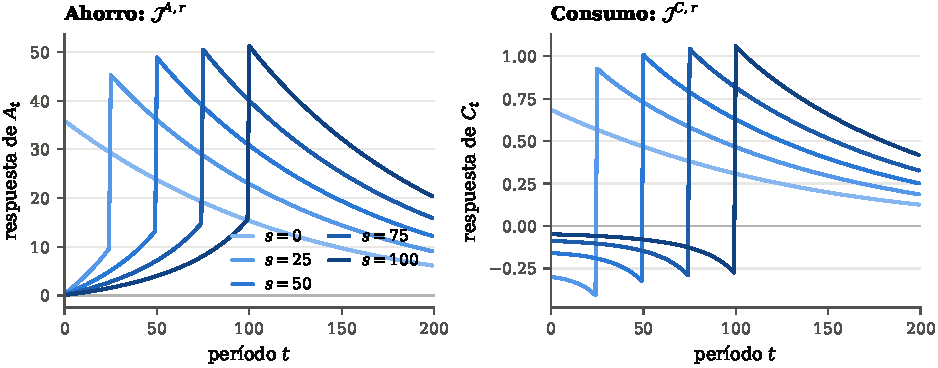
\includegraphics[width=\textwidth]{fig01_columnas_jacobiano.pdf}
\caption{Columnas del jacobiano del bloque de hogares respecto de la tasa de
interés, en el modelo de Krusell--Smith. Cada curva es la respuesta de la
variable agregada a la \emph{noticia}, recibida en la fecha $0$, de que la tasa
será un punto más alta en la fecha $s$. El patrón de ``carpa'' --- acumulación
previa al choque, pico en $s$, desacumulación posterior --- es la firma
característica de estos modelos.}
\label{fig:columnas}
\end{figure}

Vale la pena leer la figura con calma, porque contiene casi toda la economía del
modelo.

\paragraph{La columna $s=0$} Cuando la tasa sube hoy, sin aviso, los hogares
reciben un retorno mayor sobre los activos que ya tenían. Es un efecto riqueza
puro: ahorran parte de ese ingreso extra, y en los períodos siguientes lo van
desacumulando lentamente. La curva arranca en su máximo y decae.

\paragraph{Las columnas $s>0$} Aquí aparece la sustitución intertemporal. Si el
hogar sabe que la tasa será alta dentro de 50 trimestres, le conviene llegar a
esa fecha con más activos. Entonces ahorra desde hoy, acumulando
progresivamente, llega al pico justo en $s$, y después desacumula. De ahí la
``carpa''. La parte ascendente es anticipación; la descendente, el mismo efecto
riqueza de antes.

\paragraph{El consumo} El panel derecho muestra el espejo. Ante una noticia de
tasa alta futura, el consumo \emph{cae} hoy (el agente está ahorrando para
llegar con más activos) y salta en la fecha del choque. La caída inicial es
pequeña en relación con el salto: los hogares restringidos no pueden sustituir
intertemporalmente, y en esta calibración un 2.5\% de ellos están contra la
restricción de endeudamiento en todo momento.

\section{La estructura que hace posible el algoritmo rápido}

La figura \ref{fig:estructura} muestra la misma matriz de dos maneras.

\begin{figure}[htbp]
\centering
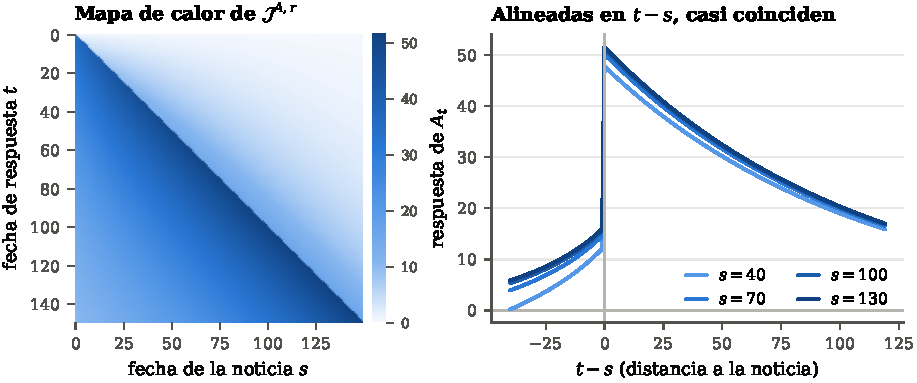
\includegraphics[width=\textwidth]{fig02_estructura_jacobiano.pdf}
\caption{Izquierda: mapa de calor de $\J^{A,r}$. Derecha: las columnas
$s=40,70,100,130$ realineadas en $t-s$. Lejos del origen, las columnas son
esencialmente traslados unas de otras: el jacobiano es asintóticamente
invariante en el tiempo.}
\label{fig:estructura}
\end{figure}

El panel derecho contiene la observación crucial. Si uno toma la columna $s=70$ y
la desplaza 30 períodos hacia la izquierda, queda casi exactamente encima de la
columna $s=100$. Formalmente,
\begin{equation}
\J_{t,s} \;\approx\; \J_{t-1,s-1} \qquad \text{para } t,s \text{ grandes}.
\label{eq:asint}
\end{equation}

¿Por qué? Dos razones independientes.

\begin{enumerate}[leftmargin=1.4em]
\item \textbf{Hacia atrás:} el comportamiento de un agente ante una noticia
depende solo de la \emph{distancia} a esa noticia, no de la fecha del
calendario. Cómo reacciona hoy a algo que pasará en 50 trimestres es lo mismo
que cómo reaccionará mañana a algo que pasará 50 trimestres después de mañana.
Esto es exacto, no aproximado, y es el lema \ref{lema:politicas} del capítulo
\ref{cap:fakenews}.
\item \textbf{Hacia adelante:} el efecto de un cambio en la distribución se
disipa. Si hoy la distribución se perturba un poco, dentro de 200 trimestres
casi no queda rastro, porque el proceso de ingreso es ergódico y la mezcla
elimina la información inicial. La figura \ref{fig:expectativa} cuantifica esa
disipación.
\end{enumerate}

La relación \eqref{eq:asint} no es solo una curiosidad estética. Significa que
la matriz $\J$, que tiene $T^2 = 90\,000$ entradas, está determinada por un
número mucho menor de objetos independientes. El algoritmo fake news es,
precisamente, el procedimiento que explota esa redundancia para calcular las
$90\,000$ entradas al costo de calcular unas $2T$.

\chapter{El bloque de agentes heterogéneos}
\label{cap:bloque}

Para poder aplicar el algoritmo rápido hay que escribir el problema individual
en una forma canónica. Este capítulo explica cuál es esa forma, por qué tiene
esa estructura y cómo se construyen sus tres piezas en la práctica.

\section{La forma canónica}

\begin{definicion}[Bloque heterogéneo]
Un bloque de agentes heterogéneos es un sistema de tres ecuaciones que mapea
una trayectoria de insumos agregados $\{X_t\}$ a una trayectoria de productos
agregados $\{Y_t\}$:
\begin{align}
v_t &= v(v_{t+1},\, X_t) \label{eq:canon-v}\\
D_{t+1} &= \Lambda(v_{t+1},\, X_t)'\, D_t \label{eq:canon-D}\\
Y_t &= y(v_{t+1},\, X_t)'\, D_t \label{eq:canon-Y}
\end{align}
donde $D_t$ es el vector $n_g\times 1$ que representa la distribución de agentes
sobre la grilla al inicio de $t$, $v_t$ es la variable de continuación (una
función de valor, su derivada, o cualquier representación equivalente),
$\Lambda$ es la matriz de transición $n_g\times n_g$ y $y$ es la matriz de
resultados individuales.
\end{definicion}

Las tres ecuaciones tienen una dirección temporal distinta y eso es esencial.

\begin{itemize}[leftmargin=1.4em]
\item \eqref{eq:canon-v} corre \textbf{hacia atrás}: para saber qué hace un
agente hoy hay que saber qué valor le asigna al futuro. Se resuelve desde
$T-1$ hacia $0$ partiendo de $v_T = v_\sst$.
\item \eqref{eq:canon-D} corre \textbf{hacia adelante}: la distribución de
mañana depende de la de hoy y de lo que la gente decida hoy. Se resuelve desde
$0$ hacia $T-1$ partiendo de $D_0 = D_\sst$.
\item \eqref{eq:canon-Y} es \textbf{instantánea}: agrega políticas individuales
contra la distribución.
\end{itemize}

\begin{idea}
Esta estructura hacia atrás/hacia adelante es el motivo por el que resolver estos
modelos cuesta caro, y también el motivo por el que el algoritmo fake news
funciona. El método directo tiene que hacer una pasada hacia atrás \emph{y} una
hacia adelante por cada columna del jacobiano: $2T$ pasadas en total. El
algoritmo fake news hace una sola pasada hacia atrás y una sola hacia adelante
para todas las columnas.
\end{idea}

\section{Construir las tres piezas}

\subsection{La iteración hacia atrás: el método del punto endógeno}

Resolver \eqref{eq:canon-v} con iteración de la función de valor es lento y poco
preciso. En la práctica se usa la ecuación de Euler y el \emph{método del punto
endógeno} de Carroll (2006), que evita resolver una ecuación no lineal en cada
punto de la grilla.

La idea es invertir el orden del problema. En lugar de preguntar ``dado
$a_-$, ¿cuánto consume el agente?'' --- que exige resolver una ecuación
implícita --- se pregunta ``si el agente termina con $a'$ activos, ¿con cuántos
tuvo que empezar?'', que es explícito. Concretamente, con $v_t \equiv \partial
V_t/\partial a_-$:

\begin{receta}
\begin{enumerate}[leftmargin=1.4em,itemsep=1pt]
\item Valor marginal esperado: $W_a(e,a') = \beta \sum_{e'} \Pi(e,e')\,v_{t+1}(e',a')$.
\item Consumo implicado por la Euler: $c^{\text{endog}}(e,a') = (W_a)^{-\sigma}$,
con $\sigma$ la elasticidad de sustitución intertemporal.
\item Recursos que lo sostienen: $\mathrm{coh}^{\text{endog}} = c^{\text{endog}} + a'$.
\item Interpolar la grilla $a'$ sobre $\mathrm{coh}^{\text{endog}}$, evaluada en
los recursos efectivos $\mathrm{coh}(e,a_-) = (1+r_t)a_- + w_t e$. Eso da la
política $a'(e,a_-)$ \emph{sobre la grilla de $a_-$}.
\item Imponer la restricción: $a' \leftarrow \max\{a', \underline{a}\}$.
\item Recuperar $c = \mathrm{coh} - a'$ y actualizar
$v_t = (1+r_t)\,c^{-1/\sigma}$ por el teorema de la envolvente.
\end{enumerate}
\end{receta}

El paso 5 es el que incorpora la no linealidad importante del modelo --- la
restricción de endeudamiento --- y es por eso que el método resuelve el problema
individual de forma \emph{global}, no perturbada. La linealización ocurre
después, y solo en los agregados.

\subsection{La matriz de transición}

Dada la política $a'(e,a_-)$, la matriz $\Lambda$ se construye en dos piezas:
la lotería de Young sobre el estado endógeno y la cadena de Markov sobre el
exógeno. Si $L$ denota la primera y $\Pi$ la segunda,
\begin{equation}
\Lambda_{(e,a_-),(e',a)} = \Pi(e,e')\, L_{a_-,a}(e),
\qquad\text{es decir}\qquad
\Lambda = L\,\Pi, \quad \Lambda' = \Pi' L'.
\end{equation}

En el código nunca se forma $\Lambda$ explícitamente --- sería una matriz de
$1\,400\times 1\,400$ o mucho peor --- sino que se aplican sus dos factores por
separado. Esto importa: la iteración hacia adelante cuesta $O(n_g)$ en lugar de
$O(n_g^2)$.

\subsection{Los resultados individuales}

$y_t$ es simplemente la colección de variables que uno quiere agregar: ahorro,
consumo, horas, crédito, reservas, lo que sea. Un detalle útil: si uno quiere
momentos de orden superior, basta definir el resultado individual como una
potencia. El segundo momento no centrado del consumo es el agregado de $c^2$, y
de ahí sale la varianza combinando dos bloques.

\section{El estado estacionario}

El estado estacionario es el punto fijo de \eqref{eq:canon-v}--\eqref{eq:canon-D}
con $X_t = X_\sst$ constante. Se resuelve en dos etapas:

\begin{enumerate}[leftmargin=1.4em]
\item Iterar \eqref{eq:canon-v} hacia atrás hasta que $v$ deje de cambiar. Esto
converge a tasa $\beta$, así que con $\beta=0.98$ hacen falta del orden de mil
iteraciones para alcanzar $10^{-11}$.
\item Iterar \eqref{eq:canon-D} hacia adelante hasta que $D$ deje de cambiar.
Esto converge a la tasa del segundo autovalor de $\Lambda$, que puede ser muy
cercana a uno si el proceso de ingreso es muy persistente. Conviene usar un
criterio en norma del supremo y no en norma dos.
\end{enumerate}

Casi siempre hay además una etapa de \emph{calibración}: elegir $\beta$ para que
la demanda agregada de activos iguale un objetivo (una relación capital--producto,
una riqueza líquida sobre ingreso). Eso es una biyección monótona y se resuelve
por bisección en pocas decenas de evaluaciones.

\begin{trampa}
Un estado estacionario mal convergido envenena todo lo que viene después, y lo
hace de forma silenciosa. Si $D_\sst$ todavía se mueve en la undécima cifra, los
jacobianos tendrán errores del orden de esa cifra dividida por el tamaño del
paso de diferenciación $h$. Con $h=10^{-4}$, un error de $10^{-11}$ en el estado
estacionario se convierte en un error de $10^{-7}$ en el jacobiano. Conviene
exigir convergencia a $10^{-14}$ en la distribución, que no cuesta casi nada.
\end{trampa}

\section{Qué modelos entran en esta forma}

Entran directamente: los modelos de ahorro precautorio con uno o varios activos;
los modelos con oferta laboral endógena; los modelos donde los insumos agregados
afectan la probabilidad de transición entre estados exógenos (por ejemplo, el
riesgo de desempleo); las representaciones no basadas en grillas (polinomios de
Chebyshev, splines); los modelos con elección discreta suavizada por choques de
gusto de valor extremo; y --- punto importante para la parte V --- los modelos
de \emph{empresas} o \emph{bancos} heterogéneos, donde el ``agente'' es una
firma y el estado endógeno es su capital o su patrimonio.

Entran con la generalización del capítulo \ref{cap:extensiones}: entrada y
salida de agentes, distribuciones representadas por parámetros, momentos no
polinómicos como cuantiles o índices de Gini, problemas con varias etapas dentro
de un período.

No entra, y conviene saberlo desde el principio: todo modelo en el que la
función de valor $v_t$ dependa \emph{directamente} de la distribución $D_t$ de
una forma que no pase por los agregados $X_t$. El ejemplo canónico son los
modelos de búsqueda laboral con negociación individual o fijación de salarios,
donde a cada trabajador le importa la distribución de ofertas que enfrentará.
La ecuación \eqref{eq:canon-v} prohíbe esa dependencia, y no es una limitación
técnica que se pueda sortear con un truco: es estructural.

\chapter{El algoritmo \emph{fake news}}
\label{cap:fakenews}

Este es el capítulo central. Contiene el resultado técnico de \ABRS\ y la receta
que se deriva de él. Vale la pena leerlo despacio: la demostración es corta y
entenderla cambia por completo la sensación de estar usando una caja negra.

\section{El punto de partida: el método directo}

Supongamos que queremos la columna $s$ del jacobiano. El procedimiento obvio es:

\begin{enumerate}[leftmargin=1.4em,itemsep=1pt]
\item Perturbar el insumo en la fecha $s$: $X^s = X_\sst + e_s\, dx$.
\item Iterar \eqref{eq:canon-v} hacia atrás desde $T-1$ hasta $0$, guardando
$v^s_t$, $\Lambda^s_t$ y $y^s_t$ para cada $t$.
\item Iterar \eqref{eq:canon-D} hacia adelante desde $D_0 = D_\sst$.
\item Agregar: $Y^s_t = (y^s_t)' D^s_t$, y formar $\J_{t,s} = (Y^s_t - Y_\sst)/dx$.
\end{enumerate}

Hay que repetirlo $T$ veces, una por columna. Con $T=300$ eso son $300$ pasadas
hacia atrás y $300$ hacia adelante, cada una de $300$ pasos: unos $180\,000$
pasos en total. En el modelo HANK de dos activos de \abrs\ eso toma 956 segundos.
El algoritmo fake news lo hace en 3.5 segundos.

\section{Primer resultado: las políticas solo dependen de la distancia}

\begin{lema}[Invariancia de las políticas]
\label{lema:politicas}
Sean $y^s_t$ y $\Lambda^s_t$ la función de resultados y la matriz de transición
en la fecha $t$ ante un choque en la fecha $s$. Entonces
\begin{equation}
y^s_t = \begin{cases} y^{T-1}_{T-1-(s-t)} & s\ge t\\ y_\sst & s<t\end{cases}
\qquad
\Lambda^s_t = \begin{cases} \Lambda^{T-1}_{T-1-(s-t)} & s\ge t\\ \Lambda_\sst & s<t\end{cases}
\label{eq:lema1}
\end{equation}
\end{lema}

La demostración es inmediata a partir de la estructura recursiva de
\eqref{eq:canon-v}: $v_t$ depende de $v_{t+1}$ y $X_t$, y nada más. Si el choque
está $s-t$ períodos en el futuro, la solución hacia atrás es idéntica sea cual
sea el valor de $t$ en el calendario. Y si el choque ya pasó ($s<t$), el agente
se comporta como en el estado estacionario, porque \eqref{eq:canon-v} no tiene
memoria del pasado.

\begin{idea}
El lema \ref{lema:politicas} vale \textbf{sin aproximación}: es cierto para
choques de cualquier tamaño, no solo infinitesimales. Y ya basta por sí solo
para eliminar $T-1$ de las $T$ pasadas hacia atrás: una sola iteración hacia
atrás, a partir de un choque en la fecha $T-1$, entrega las políticas para todas
las fechas de choque y todas las fechas de respuesta.
\end{idea}

Queda el problema de las $T$ pasadas hacia adelante. Para eso hace falta el
segundo resultado, que sí requiere infinitesimalidad.

\section{Segundo resultado: la noticia falsa}

Definamos, para $s\ge1$ y $t\ge1$,
\begin{equation}
\F_{t,s}\cdot dx \;\equiv\; dY^s_t - dY^{s-1}_{t-1}.
\label{eq:def-F}
\end{equation}
Esto compara la respuesta en $t$ a un choque en $s$ con la respuesta un período
antes a un choque un período antes. Por el lema \ref{lema:politicas}, las
políticas en ambos casos son idénticas. Uno podría conjeturar que la diferencia
es cero. No lo es, porque la \emph{distribución} también cambió.

\begin{lema}[Diferencia de respuestas]
\label{lema:fake}
Si $D_0 = D_\sst$, entonces para $dx$ infinitesimal y $s,t\ge1$,
\begin{equation}
\F_{t,s}\cdot dx = y_\sst'\,(\Lambda_\sst')^{\,t-1}\, dD^s_1 .
\label{eq:lema2}
\end{equation}
\end{lema}

\begin{proof}
Linealizando \eqref{eq:canon-Y} alrededor del estado estacionario,
$dY^s_t = y_\sst'\,dD^s_t + (dy^s_t)'\,D_\sst$. Restando la misma expresión en
$(t-1,s-1)$ y usando $dy^s_t = dy^{s-1}_{t-1}$ del lema \ref{lema:politicas},
el segundo término se cancela y queda
\begin{equation}
\F_{t,s}\cdot dx = y_\sst'\big(dD^s_t - dD^{s-1}_{t-1}\big).
\end{equation}
Ahora linealizamos \eqref{eq:canon-D}:
$dD^s_t = \Lambda_\sst'\,dD^s_{t-1} + (d\Lambda^s_{t-1})'D_\sst$. Restando su
análoga en $(t-1,s-1)$ y usando otra vez el lema \ref{lema:politicas}
($d\Lambda^s_{t-1} = d\Lambda^{s-1}_{t-2}$), el segundo término se cancela y
queda la recursión
\begin{equation}
dD^s_t - dD^{s-1}_{t-1} = \Lambda_\sst'\big(dD^s_{t-1} - dD^{s-1}_{t-2}\big).
\end{equation}
Iterando hasta la base, y usando $dD^{s-1}_0 = 0$ (porque $D_0 = D_\sst$ está
dado), se obtiene $dD^s_t - dD^{s-1}_{t-1} = (\Lambda_\sst')^{t-1} dD^s_1$,
que es \eqref{eq:lema2}.
\end{proof}

\paragraph{De dónde sale el nombre} La expresión \eqref{eq:lema2} tiene una
lectura económica preciosa. $\F_{t,s}$ es la respuesta agregada a un choque
particular: \emph{se anuncia en la fecha $0$ que el insumo cambiará en la fecha
$s$, y en la fecha $1$ el anuncio se retracta}. Los agentes reaccionan al
anuncio, lo que mueve la distribución de $D_\sst$ a $D^s_1$. Después, al saber
que era falso, vuelven a comportarse como en el estado estacionario. Entonces el
efecto sobre los agregados en toda fecha $t\ge1$ es simplemente el de haber
partido de una distribución distinta, propagado con la dinámica estacionaria.
De ahí: \emph{noticia falsa}.

\section{Los vectores de expectativa}

La expresión \eqref{eq:lema2} se simplifica con una definición.

\begin{definicion}[Vector de expectativa]
\label{def:expectativa}
$\E_t \equiv (\Lambda_\sst)^t\, y_\sst$.
\end{definicion}

Para cada punto de la grilla, $\E_t$ dice cuál es el valor esperado del resultado
$Y$ dentro de $t$ períodos para un agente que hoy está en ese punto, bajo
comportamiento de estado estacionario. Con esto, $\F_{t,s}\cdot dx = \E_{t-1}'\,dD^s_1$,
y los $\E_t$ se obtienen de una recursión trivial, $\E_t = \Lambda_\sst \E_{t-1}$
con $\E_0 = y_\sst$, que no depende del choque en absoluto.

\begin{figure}[htbp]
\centering
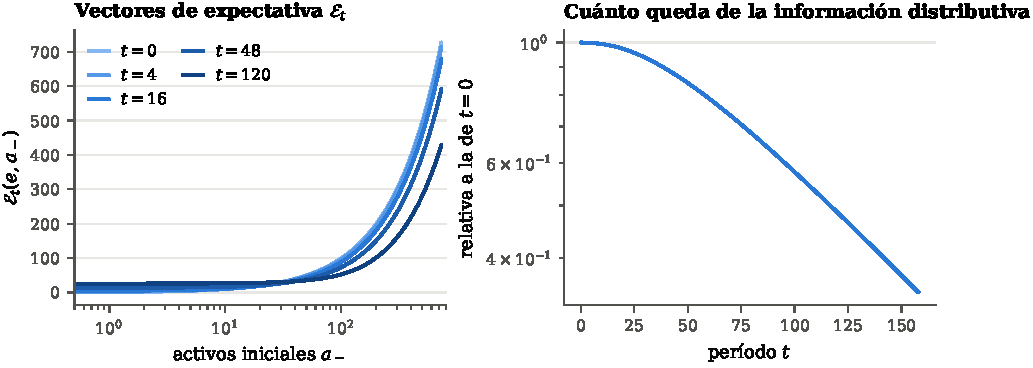
\includegraphics[width=\textwidth]{fig04_vectores_expectativa.pdf}
\caption{Izquierda: vectores de expectativa del ahorro agregado para el estado
de ingreso intermedio. Un hogar con muchos activos hoy seguirá teniendo muchos
activos dentro de cuatro trimestres, pero la relación se aplana a medida que
$t$ crece. Derecha: la dispersión de $\E_t$ entre puntos de la grilla, que mide
cuánta información sobre el agregado futuro contiene la posición actual en la
distribución. Decae, pero despacio.}
\label{fig:expectativa}
\end{figure}

El panel derecho de la figura \ref{fig:expectativa} tiene una lectura económica
directa: cuantifica cuánto tiempo ``recuerda'' la economía una perturbación de
la distribución. En esta calibración, después de 160 trimestres todavía queda
cerca de un tercio de la dispersión inicial. Esa persistencia es exactamente la
razón por la que $T$ tiene que ser grande.

\section{El resultado principal}

\begin{proposicion}[\ABRS, proposición 1]
\label{prop:principal}
Supóngase $D_0 = D_\sst$. Defínase la \emph{matriz fake news} $\F$ por
\begin{equation}
\F_{t,s}\cdot dx =
\begin{cases}
dY^s_0 & t=0\\[2pt]
\E_{t-1}'\, dD^s_1 & t\ge1
\end{cases}
\label{eq:propF}
\end{equation}
donde $dY^s_0 = (dy^s_0)'D_\sst$ y $dD^s_1 = (d\Lambda^s_0)'D_\sst$. Entonces el
jacobiano satisface la recursión
\begin{equation}
\J_{t,s} = \J_{t-1,s-1} + \F_{t,s},
\qquad\text{es decir}\qquad
\J_{t,s} = \sum_{k=0}^{\min\{s,t\}} \F_{t-k,\,s-k}.
\label{eq:recursion}
\end{equation}
\end{proposicion}

La recursión \eqref{eq:recursion} dice que cada entrada del jacobiano es la suma
de la entrada correspondiente de $\F$ y de todas las entradas de $\F$ sobre la
diagonal que va hacia arriba y a la izquierda. Por ejemplo,
$\J_{2,2} = \F_{2,2} + \F_{1,1} + \F_{0,0}$.

\begin{figure}[htbp]
\centering
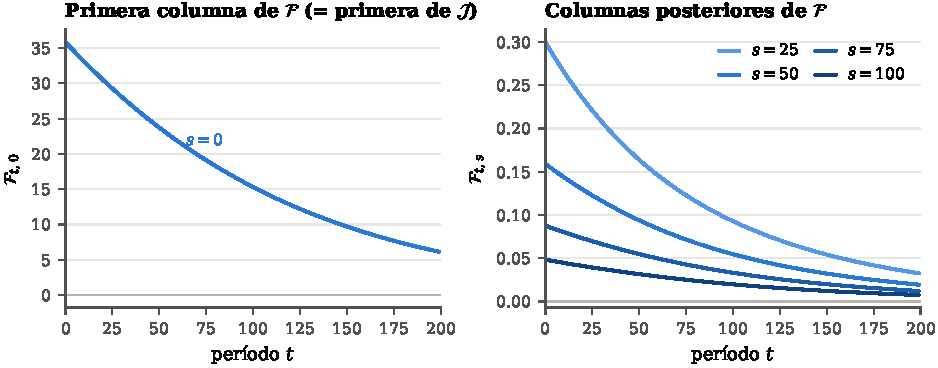
\includegraphics[width=\textwidth]{fig03_matriz_fakenews.pdf}
\caption{La matriz fake news del ahorro agregado respecto de la tasa. La primera
columna coincide con la del jacobiano. Las columnas posteriores son el efecto de
una noticia anunciada y retractada: se desacumula desde el primer período,
porque lo único que queda del anuncio es la distribución perturbada que dejó.}
\label{fig:fakenews}
\end{figure}

Comparando la figura \ref{fig:fakenews} con la \ref{fig:columnas} se ve la
economía de la descomposición. Las columnas de $\F$ son monótonas y decaen; las
de $\J$ tienen forma de carpa. La carpa aparece porque \eqref{eq:recursion}
acumula columnas desplazadas de $\F$: la acumulación previa al choque es la suma
de muchos términos pequeños de ``noticias falsas'' sucesivas.

\section{La receta}

\begin{receta}[Algoritmo fake news: un insumo y un producto]
\begin{enumerate}[leftmargin=1.4em,itemsep=3pt]
\item \textbf{Una iteración hacia atrás.} Perturbar el insumo y resolver
\eqref{eq:canon-v} hacia atrás una sola vez. De ahí salen, para cada
$s=0,\dots,T-1$:
\begin{itemize}[leftmargin=1.2em,topsep=2pt]
\item los $T$ escalares $\mathcal{Y}_s\,dx \equiv dY^s_0 = (dy^s_0)'D_\sst$:
el efecto sobre el producto \emph{hoy} de una noticia sobre la fecha $s$;
\item los $T$ vectores $\mathcal{D}_s\,dx \equiv dD^s_1 = (d\Lambda^s_0)'D_\sst$:
el efecto sobre la distribución \emph{de mañana} de esa misma noticia.
\end{itemize}
\item \textbf{Los vectores de expectativa.} $\E_0 = y_\sst$ y
$\E_t = \Lambda_\sst \E_{t-1}$ para $t=1,\dots,T-2$. No dependen del choque.
\item \textbf{Armar $\F$.} Primera fila: los $\mathcal{Y}_s$. Filas restantes:
los productos internos $\E_{t-1}'\mathcal{D}_s$. En código es un único producto
de matrices de tamaño $(T-1)\times n_g$ por $n_g \times T$.
\item \textbf{Acumular.} $\J_{t,s} = \J_{t-1,s-1}+\F_{t,s}$, recorriendo filas.
\end{enumerate}
\end{receta}

\paragraph{Varios insumos y productos} Los $\mathcal{D}_s$ dependen solo del
insumo: se calculan una vez por insumo. Los $\E_t$ dependen solo del producto:
una vez por producto. Solo los $\mathcal{Y}_s$ dependen de ambos. Por eso un
bloque con cinco insumos y cuatro productos --- veinte jacobianos --- cuesta
mucho menos que veinte veces un jacobiano.

\paragraph{Por qué es tan rápido} El método directo hace $T$ pasadas hacia atrás
y $T$ hacia adelante, cada una de $T$ pasos. El algoritmo fake news hace una
pasada hacia atrás de $T$ pasos y $T$ aplicaciones de $\Lambda_\sst$. La mejora
es de un factor $\approx T$, lo que con $T=300$ significa dos órdenes de
magnitud.


\section{El algoritmo con números: un recorrido completo}

Nada aclara tanto como ver las matrices. Esta sección ejecuta el algoritmo sobre
el bloque de hogares de Krusell--Smith con $T=6$, un horizonte absurdamente corto
pero que cabe en la página. Todas las cifras salen del código del apéndice
\ref{ap:codigo}.

\paragraph{La matriz fake news} El paso 3 produce
\begin{equation}
\F^{A,r} =
\begin{pmatrix}
35.834 & 0.636 & 0.611 & 0.589 & 0.568 & 0.548 \\
35.550 & 0.623 & 0.600 & 0.579 & 0.558 & 0.539 \\
35.268 & 0.611 & 0.589 & 0.569 & 0.549 & 0.530 \\
34.987 & 0.601 & 0.579 & 0.559 & 0.540 & 0.522 \\
34.709 & 0.590 & 0.570 & 0.550 & 0.531 & 0.514 \\
34.432 & 0.580 & 0.560 & 0.541 & 0.523 & 0.506
\end{pmatrix}
\end{equation}

Vale la pena leer su estructura antes de seguir.

\begin{itemize}[leftmargin=1.4em]
\item \textbf{La primera columna es enorme} comparada con las demás (35.8 frente
a 0.6). Es el efecto riqueza de un choque \emph{contemporáneo}: cuando la tasa
sube hoy, los hogares reciben un retorno extra sobre todo el acervo de activos
--- que es grande --- y lo ahorran casi todo.
\item \textbf{Las demás columnas son pequeñas y muy parecidas entre sí}. Son el
efecto de una noticia anunciada y retractada: los hogares ahorran un poco en el
período 0 anticipando el choque, y eso es todo lo que queda.
\item \textbf{Cada columna decae suavemente hacia abajo}. Ese decaimiento es la
disipación de la perturbación distributiva, es decir, el factor
$(\Lambda_\sst')^{t-1}$ del lema \ref{lema:fake}.
\end{itemize}

\paragraph{La acumulación} El paso 4 aplica $\J_{t,s}=\J_{t-1,s-1}+\F_{t,s}$ y da
\begin{equation}
\J^{A,r} =
\begin{pmatrix}
35.834 & 0.636 & 0.611 & 0.589 & 0.568 & 0.548 \\
35.550 & 36.457 & 1.236 & 1.190 & 1.147 & 1.107 \\
35.268 & 36.161 & 37.047 & 1.804 & 1.739 & 1.677 \\
34.987 & 35.868 & 36.741 & 37.606 & 2.344 & 2.261 \\
34.709 & 35.577 & 36.438 & 37.290 & 38.137 & 2.858 \\
34.432 & 35.289 & 36.138 & 36.979 & 37.813 & 38.643
\end{pmatrix}
\end{equation}

Ahora la matriz se ve completamente distinta, y la diferencia es instructiva.

\begin{itemize}[leftmargin=1.4em]
\item \textbf{La primera fila y la primera columna no cambiaron}: la recursión no
tiene de dónde acumular en los bordes. Esto se verifica en el código.
\item \textbf{Apareció una ``escalera'' en el triángulo inferior}, con valores
alrededor de $35$--$38$, que no estaba en $\F$. Son las columnas de $\F$
desplazadas y sumadas. Económicamente: una vez que el choque \emph{ocurrió}, el
efecto riqueza se acumuló y persiste.
\item \textbf{El triángulo superior sigue siendo pequeño} (de $0.5$ a $2.9$),
pero ahora crece al alejarse de la diagonal hacia abajo. Es la rama ascendente de
la ``carpa'' de la figura \ref{fig:columnas}: la acumulación previa al choque.
\end{itemize}

\paragraph{Verificar la recursión a mano} La proposición \ref{prop:principal}
dice que $\J_{2,2} = \F_{2,2}+\F_{1,1}+\F_{0,0}$. Con los números de arriba:
\begin{equation}
0.5895 + 0.6231 + 35.8340 = 37.0466 = \J_{2,2}. \quad\checkmark
\end{equation}
Y para una entrada fuera de la diagonal,
$\J_{4,2} = \F_{4,2}+\F_{3,1}+\F_{2,0} = 36.4377$, que es exactamente la entrada
correspondiente. Hacer esta verificación a mano con una matriz pequeña, la
primera vez que uno implementa el algoritmo, ahorra mucho tiempo después.

\begin{trampa}
Con $T=6$ el jacobiano es \emph{numéricamente} correcto pero
\emph{económicamente} inservible: supone que la economía vuelve al estado
estacionario en seis trimestres, lo que es falso. Las entradas de la esquina
inferior derecha ($38.6$) no se parecen a las del jacobiano verdadero con
$T=300$, porque allí el horizonte corto impone una condición terminal falsa. El
ejemplo sirve para ver el mecanismo, no para hacer economía.
\end{trampa}

\section{Diferenciación numérica}

En la práctica los pasos 1 y 2 se implementan con diferenciación numérica. Hay
tres opciones, en orden creciente de precisión y de esfuerzo de implementación:

\begin{enumerate}[leftmargin=1.4em]
\item \textbf{Un lado:} $(f(x+h)-f(x))/h$. Simple, error $O(h)$.
\item \textbf{Dos lados:} $(f(x+h)-f(x-h))/(2h)$. Cuesta el doble, error
$O(h^2)$, gana entre uno y dos órdenes de magnitud. Es lo que usa el código de
este manual.
\item \textbf{Diferenciación automática:} error cero, pero exige escribir el
paso hacia atrás con una librería de diferenciación automática.
\end{enumerate}

\begin{trampa}
Con diferenciación de un lado conviene usar \emph{corridas fantasma}: en lugar de
restar el valor de estado estacionario, correr el mismo código con $dx=0$ y
restar \emph{ese} resultado. Si el estado estacionario no convergió del todo, la
corrida fantasma arrastra el mismo sesgo que la perturbada y la resta lo cancela.
Es una línea de código y elimina una familia entera de errores.
\end{trampa}

\chapter{Extensiones y límites del algoritmo}
\label{cap:extensiones}

La forma canónica \eqref{eq:canon-v}--\eqref{eq:canon-Y} parece restrictiva.
En la práctica admite mucho más de lo que aparenta, con ajustes menores. Este
capítulo recorre los casos que uno se encuentra al modelar y dice, para cada
uno, si el algoritmo funciona tal cual, si hay que generalizarlo o si hay que
buscar otro método.

\section{Casos que entran sin modificar nada}

\paragraph{Adelantos del insumo} Si en lugar de $X_t$ aparece $X_{t+1}$ en el
paso hacia atrás, el algoritmo funciona sin cambios. El lema
\ref{lema:politicas} sigue valiendo, porque la iteración hacia atrás ya
incorpora el efecto de los insumos futuros a través de la continuación.

\paragraph{Momentos de orden superior} Si uno define el resultado individual como
$y^k$ en lugar de $y$, el agregado es el $k$-ésimo momento no centrado. Con dos
bloques (uno para $y$, otro para $y^2$) y un bloque simple que los combine, se
obtiene el jacobiano de la varianza. Lo mismo vale para un índice de precios CES
o para el coeficiente de variación del consumo.

\paragraph{Representaciones no basadas en grillas} Nada en el algoritmo exige
que $v$ sea un vector de valores sobre una grilla. Puede ser un vector de
coeficientes de Chebyshev o de un spline. Lo que sí tiene que ser una
distribución sobre puntos es $D$ --- y aun eso se relaja en la sección
siguiente.

\paragraph{Elección discreta con choques de gusto} Un modelo con elección
discreta (ajustar o no un bien durable, cambiar o no el precio) tiene políticas
discontinuas, y la perturbación de primer orden sobre una grilla da cero: ningún
punto de la grilla cruza el umbral ante un choque infinitesimal. La solución
estándar es añadir choques de gusto iid --- típicamente de valor extremo, que dan
probabilidades logit --- de modo que la probabilidad de cada opción varía de
forma continua con el estado. Hecho eso, el bloque entra en la forma canónica
tomando $D_t$ como la distribución \emph{antes} de la realización del choque de
gusto, y $v$, $\Lambda$, $y$ como valores esperados sobre ese choque.

\paragraph{Distribución endógena dentro del período} ¿Qué pasa si un choque en
$t$ afecta la posición de los agentes en $t$ --- por ejemplo, una ganancia de
capital sobre la riqueza, o una probabilidad de desempleo que se realiza en $t$?
La regla es: mantener $D_t$ como la distribución \emph{previa} a cualquier evento
de la fecha $t$, e incorporar esos eventos dentro de $v$, $\Lambda$ e $y$.

\begin{trampa}
\textbf{Rezagos del insumo.} Si en el paso hacia atrás aparece $X_{t-1}$, el
lema \ref{lema:politicas} \textbf{falla}: ahora el comportamiento en $t$ depende
del pasado y no solo de la distancia al choque futuro. La solución limpia no es
parchear el algoritmo, sino sacar el rezago del bloque heterogéneo: definir una
variable nueva $\tilde X_t \equiv X_{t-1}$ como producto de un bloque simple
--- que sí admite rezagos sin problema --- y pasarle $\tilde X_t$
contemporáneo al bloque heterogéneo. En el modelo de Krusell--Smith del
capítulo \ref{cap:jacobiano}, el rezago del capital vive en el bloque de
empresas por exactamente esta razón.
\end{trampa}

\section{La generalización: productos y transiciones no lineales}

Algunos modelos necesitan reemplazar \eqref{eq:canon-D} y \eqref{eq:canon-Y} por
funciones generales de la distribución:
\begin{align}
D_{t+1} &= \mathcal{D}(v_{t+1}, X_t, D_t),\\
Y_t &= \mathcal{Y}(v_{t+1}, X_t, D_t).
\end{align}

\begin{proposicion}[\ABRS, proposición 2]
\label{prop:general}
Con esas dos ecuaciones generales, la proposición \ref{prop:principal} sigue
valiendo si se redefine el vector de expectativa como
\begin{equation}
\E_t \equiv (\mathcal{D}_D')^{\,t}\,\mathcal{Y}_D',
\label{eq:E-general}
\end{equation}
donde $\mathcal{D}_D$ es el jacobiano $n_g\times n_g$ de $\mathcal{D}$ respecto de
$D$ y $\mathcal{Y}_D$ el gradiente de $\mathcal{Y}$ respecto de $D$, ambos
evaluados en el estado estacionario.
\end{proposicion}

La demostración es la misma del lema \ref{lema:fake} reemplazando $\Lambda_\sst'$
por $\mathcal{D}_D$ y $y_\sst'$ por $\mathcal{Y}_D$. El contenido económico es
transparente: $\mathcal{D}_D$ es el ``operador de propagación'' de una
perturbación distributiva y $\mathcal{Y}_D$ es el ``operador de lectura'' del
agregado. En el caso lineal original, esos dos operadores son $\Lambda_\sst'$ e
$y_\sst'$.

Esto abre tres casos útiles.

\paragraph{Entrada y salida de agentes} Si los agentes salen con probabilidad
$1-\varsigma$ y entran con una distribución fija $\Psi$,
\begin{equation}
D_{t+1} = \varsigma\, \Lambda(v_{t+1},X_t)'\,D_t + (1-\varsigma)\,\Psi .
\end{equation}
Entonces $\mathcal{D}_D = \varsigma\,\Lambda'_\sst$ y $\mathcal{Y}_D = y_\sst'$. La
única consecuencia práctica es que los vectores de expectativa se descuentan por
la supervivencia: $\E_t = \varsigma^t \Lambda_\sst^t y_\sst$. Todo lo demás del
algoritmo queda igual. Este es el caso de los modelos de dinámica de empresas y
de los modelos bancarios tipo Gertler--Karadi, y es el que usamos en la parte V.

\paragraph{Distribuciones paramétricas} Si $D_t$ es un vector de parámetros que
describe una densidad en lugar de masas sobre puntos, basta con poder calcular
$\mathcal{D}_D$ y $\mathcal{Y}_D$, típicamente por diferenciación numérica.

\paragraph{Momentos no polinómicos} Un cuantil, un índice de Gini, una razón
entre percentiles: todos son funciones no lineales de $D$, y el algoritmo los
admite vía $\mathcal{Y}_D$. Con una distribución discretizada el cuantil es una
función escalonada y su derivada no sirve; la solución es interpolarla
linealmente entre puntos de masa, lo que da un gradiente analítico sencillo.

\section{Lo que no entra}

Hay una restricción que la generalización no levanta: la proposición
\ref{prop:general} deja intacta la ecuación \eqref{eq:canon-v}. La variable de
continuación $v_t$ \textbf{no puede depender de $D_t$}.

Económicamente, eso excluye todo modelo en el que a un agente le importe
directamente la distribución futura de otros agentes, de una forma que no pase
por un precio o agregado $X_t$. Los ejemplos de la literatura son:

\begin{itemize}[leftmargin=1.4em]
\item modelos de generaciones superpuestas con herencias endógenas recibidas a
mitad de la vida;
\item modelos de búsqueda laboral con publicación de salarios o negociación
individual, donde importa la distribución de ofertas;
\item modelos de búsqueda monetaria donde importa la distribución de saldos
de efectivo de las contrapartes.
\end{itemize}

\begin{tutesis}
Vale la pena chequear esta condición en tu modelo, porque está más cerca de lo
que parece. Si el mercado interbancario se modelara con \emph{búsqueda y
negociación bilateral} al estilo de Afonso y Lagos (2015), a cada banco le
importaría la distribución de posiciones de liquidez de sus contrapartes
potenciales, y la condición fallaría. Tu plan de trabajo evita ese problema
\emph{por construcción}: la regla proporcional $\psi_k = \tau_k \min(1, P/Q)$
hace que toda la información del mercado llegue al banco a través de dos
escalares agregados, $P$ y $Q$. Esa simplificación, que el plan justifica como
``una aproximación reducida'', resulta ser además exactamente la condición que
hace aplicable el método. Conviene decirlo explícitamente cuando defiendas esa
elección de modelado: no es solo tratabilidad, es lo que mantiene el modelo
dentro de la clase resoluble.
\end{tutesis}

\section{Varias etapas dentro de un período}

Un caso frecuente en macrofinanzas: dentro del período $t$ pasan varias cosas en
orden --- primero se eligen carteras, después se realiza un choque, después hay
un mercado que redistribuye liquidez, después se paga. Modelar eso metiendo
todo dentro de $v$, $\Lambda$, $y$ se vuelve rápidamente ilegible.

La generalización natural es permitir varias \emph{etapas} por período, cada una
con su propio operador de transición, y encadenarlas. El algoritmo se aplica
tratando la composición de etapas como un único $\mathcal{D}$. En la práctica, si
una de las etapas es un mercado cuyo precio se determina por vaciado, la forma
más simple de proceder es la del capítulo \ref{cap:dag}: declarar ese precio
como incógnita agregada y su condición de vaciado como objetivo, y dejar que el
sistema de equilibrio general lo resuelva simultáneamente.


\part{Del bloque al equilibrio general}
\chapter{Del bloque al equilibrio general}
\label{cap:dag}

Tener el jacobiano del bloque heterogéneo no es tener el modelo. Falta
combinarlo con las empresas, el gobierno, los mercados y las reglas de política.
Este capítulo explica cómo, y cómo hacerlo de manera que escale.

\section{El equilibrio como un sistema de ecuaciones}

Todo modelo de equilibrio general en el espacio de secuencias se escribe
\begin{equation}
\mathbf{F}(\mathbf{X}, \mathbf{Z}) = \mathbf{0},
\label{eq:F}
\end{equation}
con tantas ecuaciones como variables endógenas. Truncado en $T$, es un sistema
de $n_x \times T$ ecuaciones. La solución a primer orden es
$d\mathbf{X} = -\mathbf{F}_X^{-1}\mathbf{F}_Z\,d\mathbf{Z}$.

El problema es el tamaño. Un modelo DSGE cuantitativo tiene fácilmente veinte o
treinta variables endógenas; con $T=300$, la matriz $\mathbf{F}_X$ es de
$9\,000\times 9\,000$ y su inversión empieza a dominar el costo total. Peor: el
sistema es innecesariamente grande, porque muchas de esas ecuaciones son
definiciones que se pueden sustituir.

\section{Sustitución de variables y el grafo}

La solución es separar las ecuaciones en dos grupos. Las que se pueden resolver
explícitamente --- la función de producción, las condiciones de primer orden de
la empresa, la restricción presupuestaria del gobierno --- se usan para expresar
variables en función de otras. Lo que queda es un sistema reducido
\begin{equation}
\mathbf{H}(\mathbf{U}, \mathbf{Z}) = \mathbf{0},
\label{eq:H}
\end{equation}
con $n_u \ll n_x$ \emph{incógnitas} y el mismo número de \emph{objetivos}.
La solución es entonces
\begin{equation}
d\mathbf{U} = -\mathbf{H}_U^{-1}\mathbf{H}_Z\,d\mathbf{Z},
\qquad
d\mathbf{X} = \mathbf{M}_U\,d\mathbf{U} + \mathbf{M}_Z\,d\mathbf{Z},
\end{equation}
donde $\mathbf{M}$ recupera el resto de las variables.

La forma sistemática de organizar esas sustituciones es un \emph{grafo acíclico
dirigido} (DAG). Cada pieza del modelo es un \emph{bloque} con insumos y
productos; se dibuja una flecha de un bloque a otro cuando un producto del
primero es insumo del segundo.

\begin{definicion}[Modelo en el espacio de secuencias]
Un modelo consta de: un conjunto de choques exógenos $\mathcal{Z}$, un conjunto
de incógnitas $\mathcal{U}$, un conjunto de productos $\mathcal{O}$ de los cuales
un subconjunto $\mathcal{H}$ son objetivos, y una colección de bloques --- simples
o heterogéneos --- tales que cada producto pertenece a exactamente un bloque, el
número de incógnitas iguala el de objetivos, y el grafo resultante es acíclico.
Un equilibrio es una asignación de secuencias tal que cada bloque se satisface y
todos los objetivos valen cero.
\end{definicion}

\paragraph{Bloques simples} Un bloque simple es cualquier mapeo
$Y_t = h(X_{t-k},\dots,X_{t+l})$ entre secuencias. Sus jacobianos son matrices
de banda y se obtienen por diferenciación numérica a costo despreciable: $T$
evaluaciones de una función vectorizada por insumo.

\paragraph{Por qué acíclico} La aciclicidad permite ordenar los bloques
(\emph{orden topológico}) de modo que al evaluar cada uno todos sus insumos ya
están calculados. Eso vuelve mecánica la aplicación de la regla de la cadena.

\begin{idea}
La aciclicidad \textbf{no} restringe el modelo económico, solo su representación.
Si hay simultaneidad genuina --- el bloque $b_1$ necesita un producto de $b_3$ y
$b_3$ necesita uno de $b_1$ --- siempre se puede romper el ciclo declarando esa
variable como \emph{incógnita} adicional y su condición de consistencia como
\emph{objetivo} adicional. No se itera: el sistema lineal la resuelve junto con
todo lo demás.
\end{idea}

\section{Acumulación hacia adelante}

Con el grafo ordenado, los jacobianos totales se construyen por
\emph{acumulación hacia adelante}, que es la aplicación sistemática de la regla
de la cadena. Sea $\mathbf{J}^{o,i}$ el jacobiano \emph{total} del producto $o$
respecto del choque o incógnita $i$, y $\J^{o,m}$ el jacobiano \emph{parcial} del
bloque que produce $o$ respecto de su insumo directo $m$. Se inicializa
$\mathbf{J}^{i,i} = I$ para cada $i \in \mathcal{Z}\cup\mathcal{U}$ y se recorren
los bloques en orden topológico aplicando
\begin{equation}
\mathbf{J}^{o,i} = \sum_{m\,\in\, \text{insumos del bloque}} \J^{o,m}\,\mathbf{J}^{m,i}.
\label{eq:forward}
\end{equation}

Al terminar, $\mathbf{H}_U$ y $\mathbf{H}_Z$ son los jacobianos totales de los
objetivos respecto de las incógnitas y de los choques. Se apilan, se invierte, y
el modelo está resuelto.

\begin{trampa}
La distinción entre jacobiano \emph{parcial} y \emph{total} es sutil y causa
errores conceptuales serios. En un modelo HANK, $\J^{N,w}$ (parcial) es cuánto
cambia la oferta laboral ante un cambio del salario manteniendo todo lo demás
fijo; $\mathbf{J}^{N,w}$ (total) incluye además que un salario mayor reduce los
beneficios de las empresas, lo que reduce los dividendos que reciben los hogares,
lo que a su vez mueve la oferta laboral. Son objetos distintos y el que entra en
$\mathbf{H}_U$ es el total.
\end{trampa}

\section{Un ejemplo completo: Krusell--Smith}

El modelo del capítulo \ref{cap:jacobiano} tiene tres bloques:

\begin{enumerate}[leftmargin=1.4em,itemsep=1pt]
\item \textbf{empresas} (simple): toma $(K, Z)$ y devuelve $(r, w, Y)$ usando
$r_t = \alpha Z_t (K_{t-1}/N)^{\alpha-1} - \delta$ y
$w_t = (1-\alpha)Z_t(K_{t-1}/N)^{\alpha}$.
\item \textbf{hogares} (heterogéneo): toma $(r,w)$ y devuelve $(A, C)$. Sus
jacobianos son los de la figura \ref{fig:columnas}.
\item \textbf{vaciado} (simple): toma $(A,K)$ y devuelve el residuo $A - K$.
\end{enumerate}

Hay un choque ($Z$), una incógnita ($K$) y un objetivo (el vaciado del mercado de
activos). Las variables $r$ y $w$ quedan sustituidas: no son incógnitas. El
sistema completo es de $300\times300$, se invierte en milisegundos, y entrega la
matriz $\mathbf{G}$ que mapea cualquier trayectoria de productividad a la
respuesta de cualquier variable.

\begin{figure}[htbp]
\centering
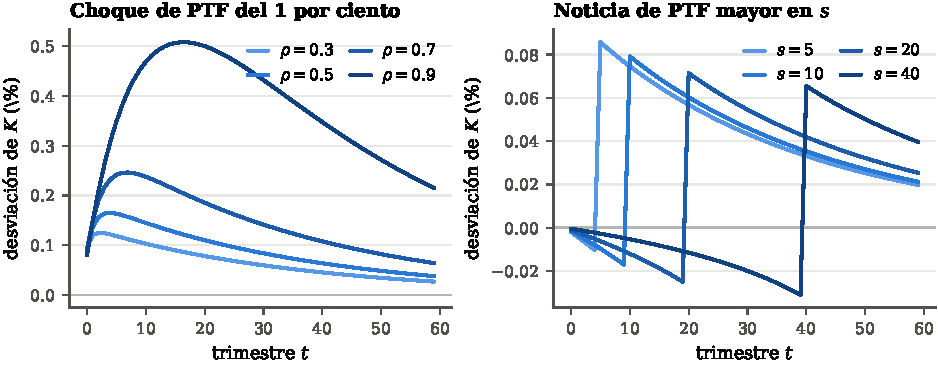
\includegraphics[width=\textwidth]{fig07_irf_krusell_smith.pdf}
\caption{Funciones impulso-respuesta del capital en el modelo de Krusell--Smith.
Izquierda: choques AR(1) de productividad del 1\%, con distinta persistencia.
Derecha: noticias de que la productividad será 1\% mayor en la fecha $s$.
Ambos paneles usan la \emph{misma} matriz $\mathbf{G}$; calcular una respuesta
adicional cuesta un producto matriz--vector.}
\label{fig:irf-ks}
\end{figure}

Dos verificaciones que conviene hacer siempre, y que esta solución pasa. Primero,
en impacto el producto responde exactamente 1\% ante un choque de 1\% de
productividad, porque el capital está predeterminado: $dY_0/Y = dZ_0/Z$ sin
importar la persistencia. Segundo, la tasa de interés sube exactamente
$\alpha\,dZ_0\,(K_\sst/N)^{\alpha-1} = 3.60$ puntos básicos en impacto, también
independiente de $\rho$. Que el código reproduzca estas dos identidades analíticas
es una señal fuerte de que el grafo está bien armado.

\section{Determinación y diagnóstico}
\label{sec:diagnostico}

El modelo tiene solución local única si $\mathbf{H}_U$ es invertible. En la
práctica conviene no confiar en que la inversión ``funcione'' y mirar tres cosas:

\begin{receta}[Diagnóstico del sistema de equilibrio]
\begin{enumerate}[leftmargin=1.4em,itemsep=2pt]
\item \textbf{Número de condición de $\mathbf{H}_U$.} Si está por encima de
$10^{10}$, el sistema está casi singular y la solución es ruido. Causa habitual:
una ecuación redundante (haber impuesto la ley de Walras \emph{y} todas las
condiciones de vaciado).
\item \textbf{Sensibilidad a $T$.} Resolver con $T$ y con $1.5T$ y comparar. Si
la respuesta cambia, $T$ es demasiado corto (capítulo \ref{cap:precision}).
\item \textbf{Identidades analíticas conocidas.} Casi todo modelo tiene alguna
respuesta que se puede calcular a mano: la respuesta en impacto de una variable
predeterminada, una restricción presupuestaria agregada, la suma de dos
jacobianos que debe dar cero. Verificarlas atrapa la mayoría de los errores de
armado.
\end{enumerate}
\end{receta}

\begin{trampa}
En el bloque de hogares del modelo de Krusell--Smith se cumple, exactamente, que
$\J^{C,w}_{0,0} + \J^{A,w}_{0,0} = \Ex[e] = 1$: un sol más de salario hoy se
consume o se ahorra, no se evapora. Y para toda noticia sobre el futuro,
$\J^{C,w}_{0,s} + \J^{A,w}_{0,s} = 0$: una noticia no cambia los recursos de hoy,
solo cómo se reparten. El código de este manual verifica ambas identidades como
parte de sus pruebas, y se cumplen hasta $10^{-6}$. Si en tu modelo no se
cumplen, hay un error de contabilidad en el paso hacia atrás, no un problema
numérico.
\end{trampa}

\chapter{Precisión numérica y verificación}
\label{cap:precision}

Un método rápido que da el número equivocado no sirve de nada. Este capítulo
trata de cómo saber que el resultado es correcto, que es la parte del trabajo
que más se omite y la que más caro sale omitir.

\section{Las tres fuentes de error}

\begin{enumerate}[leftmargin=1.4em]
\item \textbf{Discretización.} La grilla y la cadena de Markov aproximan un
modelo continuo. Este error existe antes de aplicar ningún método de solución y
es compartido con cualquier alternativa.
\item \textbf{Diferenciación.} Si se usa diferenciación numérica en lugar de
automática, hay un error de orden $h$ (un lado) o $h^2$ (dos lados).
\item \textbf{Truncamiento.} Se resuelve un sistema de horizonte $T$ en lugar de
infinito.
\end{enumerate}

Solo la segunda y la tercera son propias del método. Vale la pena tratarlas por
separado, porque los remedios son distintos.

\section{Verificar contra el método directo}

La prueba más importante, y la que hay que correr siempre que se escribe un
bloque nuevo, es comparar el algoritmo fake news contra el método directo. El
método directo es lento pero no depende de la proposición \ref{prop:principal}:
simplemente perturba y resuelve la transición completa. Si ambos coinciden, el
bloque está bien escrito.

\begin{figure}[htbp]
\centering
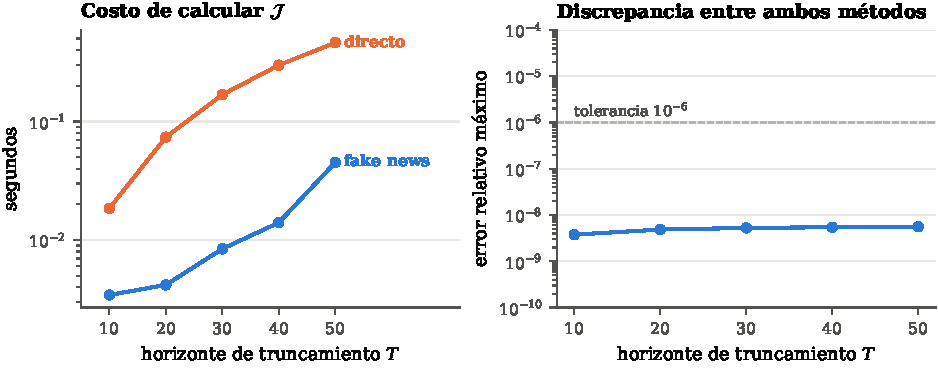
\includegraphics[width=\textwidth]{fig05_verificacion.pdf}
\caption{Izquierda: tiempo de cómputo de los dos métodos en el bloque de hogares
de Krusell--Smith con 100 puntos de activos. El método directo escala como $T^2$
y el algoritmo fake news esencialmente como $T$. Derecha: discrepancia máxima
relativa entre ambos. El error se mantiene en el orden de $5\times10^{-9}$, que
es el límite de la diferenciación numérica de dos lados, no un error del
algoritmo.}
\label{fig:verificacion}
\end{figure}

La figura \ref{fig:verificacion} muestra el resultado para el modelo de este
manual. Con diferenciación de dos lados y $h=10^{-4}$, la discrepancia relativa
máxima sobre los cuatro jacobianos ($\J^{A,r}$, $\J^{A,w}$, $\J^{C,r}$,
$\J^{C,w}$) es de $5.5\times 10^{-9}$. El artículo original, usando
diferenciación automática, obtiene coincidencia a precisión de máquina; es decir,
la proposición \ref{prop:principal} es exacta y toda la discrepancia residual
viene de las derivadas numéricas.

\begin{receta}[Verificación mínima de un bloque nuevo]
\begin{enumerate}[leftmargin=1.4em,itemsep=2pt]
\item Resolver el estado estacionario y chequear que las restricciones
contables se cumplan \emph{exactamente} (el presupuesto agregado, la suma de la
distribución igual a uno).
\item Calcular los jacobianos con fake news y con el método directo a un
horizonte corto ($T=30$ o $T=40$, donde el directo todavía es barato) y comparar.
Exigir error relativo menor que $10^{-6}$.
\item Verificar las identidades analíticas que el modelo implique.
\item Recién entonces subir a $T=300$ y resolver el equilibrio general.
\end{enumerate}
\end{receta}

El paso 2 es barato: a $T=40$ el método directo tarda menos de un segundo. No
hay excusa para saltárselo, y saltárselo es la razón número uno por la que la
gente publica resultados equivocados con este método.

\section{Elegir el horizonte de truncamiento}

El horizonte $T$ tiene que ser lo bastante largo para que \emph{tanto el choque
como la respuesta endógena} hayan vuelto esencialmente al estado estacionario.
Son dos condiciones distintas y la segunda es la que se olvida.

\begin{figure}[htbp]
\centering
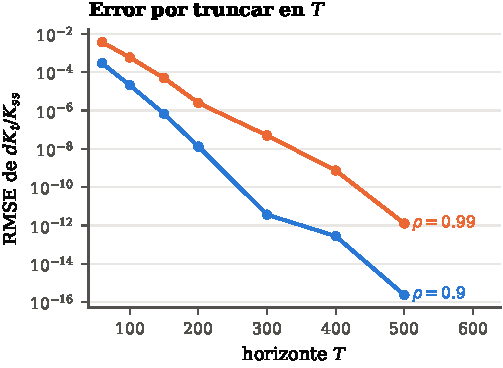
\includegraphics[width=0.52\textwidth]{fig06_truncamiento.pdf}
\caption{Error de la respuesta del capital en los primeros 60 trimestres,
medido contra una solución de referencia con $T=600$, en función del horizonte
de truncamiento. Con un choque de persistencia $\rho=0.9$ bastan unos 150
trimestres para alcanzar precisión de doce cifras; con $\rho=0.99$ hace falta
bastante más.}
\label{fig:truncamiento}
\end{figure}

La figura \ref{fig:truncamiento} cuantifica el punto. Con $\rho=0.9$ el choque
mismo ya es despreciable hacia el trimestre 100, y el error cae muy rápido. Con
$\rho=0.99$ el choque conserva el 5\% de su magnitud inicial en el trimestre
300, y el error cae mucho más despacio. Modelos con alta persistencia
\emph{interna} --- como los HANK de dos activos, donde la cartera ilíquida se
ajusta lentamente --- son más exigentes todavía.

\begin{receta}[Elegir $T$]
\begin{enumerate}[leftmargin=1.4em,itemsep=1pt]
\item Verificar que el choque mismo sea numéricamente cero en $T$.
\item Verificar que la respuesta endógena de interés sea numéricamente cero en
$T$.
\item Resolver con $T$ y con $1.5T$; si la respuesta en los primeros períodos
cambia de forma apreciable, $T$ es corto.
\end{enumerate}
\end{receta}

\section{Elegir el paso de diferenciación}

Con diferenciación numérica hay un compromiso clásico: $h$ demasiado grande
introduce error de truncamiento de Taylor; $h$ demasiado pequeño amplifica el
error de redondeo. Para diferenciación de dos lados, el óptimo está alrededor de
$h \approx \epsilon^{1/3}\approx 6\times10^{-6}$ en aritmética de doble
precisión, pero en la práctica conviene algo mayor, del orden de $10^{-4}$,
porque el ``ruido'' de la función no es el épsilon de máquina sino la tolerancia
con que convergió el estado estacionario.

\begin{trampa}
Si uno baja $h$ y el jacobiano \emph{empeora} en lugar de mejorar, el
diagnóstico casi seguro es que el estado estacionario está mal convergido: el
ruido del punto base domina la señal de la derivada. La respuesta no es ajustar
$h$ sino converger mejor el estado estacionario.
\end{trampa}

\section{Quiebres, esquinas y lo que la linealización no ve}
\label{sec:quiebres}

Hay una condición que se verifica poco y que invalida el método cuando falla: el
modelo tiene que ser \emph{diferenciable en el estado estacionario}. Las
funciones $\max$, $\min$ y $(\cdot)^+$ son omnipresentes en macrofinanzas y no
son diferenciables en su quiebre.

Hay dos situaciones y conviene no confundirlas.

\paragraph{El estado estacionario está estrictamente dentro de una rama} Si
$\min(1, P/Q)$ se evalúa en un estado estacionario donde $P/Q = 0.36$, la función
es localmente idéntica a $P/Q$ y es suave. No hay problema: basta verificarlo.

\paragraph{El estado estacionario está exactamente en el quiebre} Entonces la
derivada no existe y el método no es aplicable. Hay que recalibrar para salir del
quiebre, o cambiar de método.

Pero hay un tercer caso, más interesante, que es la razón por la que estos
modelos funcionan mucho mejor de lo que uno temería.

\begin{idea}
\textbf{La integración suaviza los quiebres.} Si $x$ es una variable aleatoria
con densidad continua, entonces $\Ex[(x+\mu)^+]$ es una función \emph{derivable
con continuidad} de $\mu$, aunque $(\cdot)^+$ no lo sea. En efecto,
\begin{equation}
\frac{\partial}{\partial\mu}\,\Ex\big[(x+\mu)^+\big] = \Pr(x+\mu > 0),
\end{equation}
que es continua si la densidad lo es. El quiebre individual no sobrevive a la
agregación sobre un continuo.
\end{idea}

\begin{figure}[htbp]
\centering
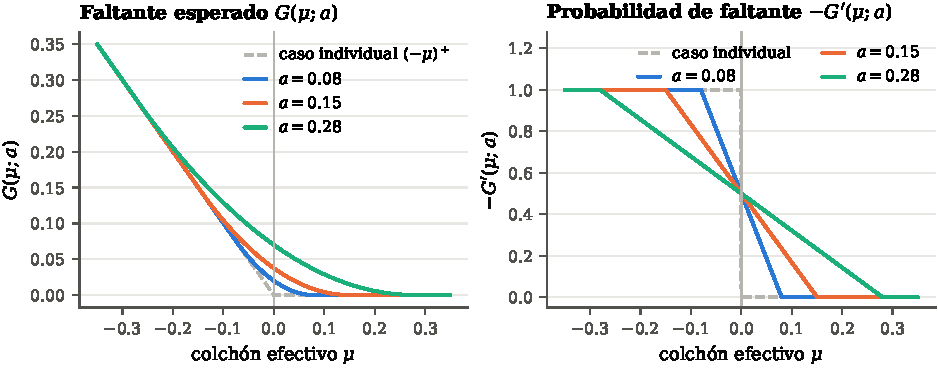
\includegraphics[width=\textwidth]{fig08_quiebre_esperanza.pdf}
\caption{El faltante de liquidez esperado por unidad de depósitos, con un choque
uniforme en $[-a,a]$. La línea punteada es el caso individual $(-\mu)^+$, con su
quiebre en cero. Las curvas sólidas son la esperanza, que es suave; su derivada
(panel derecho) es la probabilidad de faltante, continua y decreciente. Cuanto
mayor la dispersión $a$, más suave la función.}
\label{fig:quiebre}
\end{figure}

La figura \ref{fig:quiebre} ilustra el punto con la función que aparece en la
parte V. Dos lecturas adicionales que conviene extraer:

\begin{itemize}[leftmargin=1.4em]
\item La función \emph{límite} cuando $a\to 0$ es el caso individual con su
quiebre. Es decir, la suavidad se compra con dispersión: un modelo con muy poca
heterogeneidad idiosincrática está numéricamente cerca de un quiebre, aunque
formalmente sea suave.
\item La agregación suaviza \emph{dos veces}: sobre el choque idiosincrático y
sobre la distribución de agentes. Un agregado sobre bancos con distintos
umbrales es suave aunque cada banco individual tenga un umbral neto.
\end{itemize}

\begin{tutesis}
Esto responde una objeción que seguramente te van a hacer al pasar a dinámico:
``tu modelo está lleno de $\max\{x,0\}$, ¿cómo lo linealizas?''. La respuesta
corta: lo que entra en el modelo no es $\max\{x,0\}$ sino
$\Ex[\max\{x,0\}]$, y esa función es $C^1$ siempre que $F_k$ sea continua ---
que es exactamente el supuesto que tu Anexo IV ya hace. La respuesta larga tiene
una advertencia: la decisión de \emph{colchón voluntario} sí puede estar en una
esquina ($u^c = 0$), y ahí la derivada es cero por un lado y distinta de cero
por el otro. Hay que verificar en qué lado está cada tipo de banco en el estado
estacionario, y reportarlo. La sección \ref{sec:regimenes} lo hace para el
prototipo.
\end{tutesis}


\part{Qué hacer con los jacobianos}
\chapter{Qué se puede leer en un jacobiano}
\label{cap:usos}

Los jacobianos no son solo un paso intermedio para llegar a las funciones
impulso-respuesta. Son objetos económicos con contenido propio, y aprender a
leerlos es una de las habilidades más transferibles que da este método.

\section{Funciones impulso-respuesta y descomposiciones}

Lo básico ya está dicho: $d\mathbf{X} = \mathbf{G}\,d\mathbf{Z}$, y calcular una
respuesta adicional cuesta un producto matriz--vector. Dos usos menos obvios:

\paragraph{Descomponer una respuesta en canales} Supongamos que el consumo
responde a una política monetaria a través de tres canales: el efecto directo de
la tasa, el efecto ingreso vía salarios, y el efecto vía dividendos. Como la
respuesta total es
$d\mathbf{C} = \J^{C,r}d\mathbf{r} + \J^{C,w}d\mathbf{w} + \J^{C,d}d\mathbf{d}$,
basta con evaluar cada término por separado usando las respuestas de equilibrio
general $d\mathbf{r}$, $d\mathbf{w}$, $d\mathbf{d}$. La suma es exacta, no
aproximada, porque el modelo es lineal.

\paragraph{Contrafactuales de ``apagar un canal''} ¿Qué pasaría si los hogares no
respondieran a la tasa de interés? Se resuelve el equilibrio general reemplazando
$\J^{C,r}$ por cero y dejando todo lo demás igual. Esto es un experimento
coherente y barato, y es muchísimo más informativo que comparar dos
calibraciones distintas.

\section{Los jacobianos como estadísticos suficientes}

El resultado conceptual más importante de esta literatura es que, para una clase
amplia de preguntas, lo único que hace falta saber del lado de los hogares es un
jacobiano. Auclert, Rognlie y Straub (2018) muestran que en una clase de modelos
keynesianos la respuesta del producto a la política fiscal depende del modelo de
hogares \emph{solo} a través de $\J^{C,y}$, la matriz de propensiones marginales
a consumir intertemporales (las ``iMPC'').

Esto tiene dos consecuencias prácticas.

\begin{enumerate}[leftmargin=1.4em]
\item \textbf{Se puede disciplinar el modelo con microdatos.} La primera columna
de $\J^{C,y}$ es el perfil de respuesta del consumo a una transferencia
inesperada: exactamente lo que estiman los estudios de reembolsos tributarios y
loterías. Un modelo cuyo $\J^{C,y}$ no reproduce esos perfiles está mal
calibrado, aunque reproduzca la distribución de riqueza.
\item \textbf{Se pueden comparar modelos sin resolverlos.} Dos modelos con el
mismo $\J^{C,y}$ dan las mismas respuestas agregadas. Si un modelo con dos
activos y uno con un activo tienen jacobianos parecidos, la complejidad adicional
no está comprando nada para esa pregunta.
\end{enumerate}

\begin{idea}
Cuando leas un artículo con un modelo HANK complicado, la primera pregunta útil
no es ``¿cómo calibraron el proceso de ingreso?'' sino ``¿cómo se ve
$\J^{C,y}$?''. Si el artículo no lo muestra, pedirlo es la mejor pregunta que
puedes hacer en un seminario.
\end{idea}

\section{Leer la forma de un jacobiano}

Con algo de práctica, la forma de la matriz dice qué mecanismo domina. Un
catálogo breve:

\begin{itemize}[leftmargin=1.4em]
\item \textbf{Filas constantes} (como en \eqref{eq:jac-ri}): suavizamiento
perfecto, el agente solo mira valores presentes. Es el caso de ingreso
permanente.
\item \textbf{Diagonal dominante}: restricciones de liquidez. El agente responde
a lo que pasa hoy mucho más que a lo que pasa mañana, porque no puede trasladar
recursos. Cuanto más alta la fracción de restringidos, más dominante la diagonal.
\item \textbf{Columnas en forma de carpa}: sustitución intertemporal con
anticipación, como en la figura \ref{fig:columnas}.
\item \textbf{Triangular inferior}: no hay anticipación. Si esto aparece en un
bloque donde debería haber agentes prospectivos, es un error de programación.
\item \textbf{Primera fila igual a cero salvo en $s=0$}: los agregados de hoy
dependen solo de los insumos de hoy y de la distribución predeterminada. Es la
firma de una variable de acervo.
\end{itemize}

El último caso aparece en la parte V y conviene retenerlo, porque es una
verificación gratuita: si una variable agregada está determinada por el acervo
heredado, ninguna noticia sobre el futuro puede moverla hoy.

\section{La matriz de equilibrio general $\mathbf{G}$}

Después de resolver, $\mathbf{G}^{o,z}$ es una matriz $T\times T$ cuya columna
$s$ es la respuesta de equilibrio general de la variable $o$ a una noticia de que
el choque $z$ ocurrirá en $s$. Es útil pensarla como ``todas las funciones
impulso-respuesta del modelo, a la vez''.

Dos diferencias importantes respecto del jacobiano parcial $\J$:

\begin{itemize}[leftmargin=1.4em]
\item $\mathbf{G}$ incorpora la retroalimentación de precios. $\J^{C,r}$ dice
cómo responde el consumo si la tasa cambia; $\mathbf{G}^{C,Z}$ dice cómo responde
el consumo cuando la productividad cambia \emph{y} la tasa se ajusta en
equilibrio.
\item $\mathbf{G}$ depende de todo el modelo; $\J$ solo del bloque. Si cambia la
regla de política monetaria, $\mathbf{G}$ cambia y $\J$ no. Es exactamente la
distinción que la crítica de Lucas vuelve relevante, y el método la hace
operativa: los objetos invariantes a la política son los jacobianos de bloque.
\end{itemize}

\chapter{Estimación}
\label{cap:estimacion}

Aquí es donde el método paga su inversión. Estimar un modelo de agentes
heterogéneos sobre series de tiempo era, hasta hace poco, prohibitivo. Con
jacobianos secuenciales es cuestión de minutos.

\section{Del jacobiano a la representación de medias móviles}

El punto de partida es \eqref{eq:ma}. Si los choques exógenos siguen procesos de
medias móviles independientes,
\begin{equation}
d\tilde{Z}_t = \sum_{s\ge0} dZ_s\,\epsilon_{t-s},
\end{equation}
con $\epsilon_t$ innovaciones normales iid, entonces por equivalencia cierta las
variables endógenas siguen
\begin{equation}
d\tilde{X}_t = \sum_{s=0}^{T-1} dX_s\,\epsilon_{t-s},
\qquad dX = \mathbf{G}\,dZ.
\end{equation}
Es decir, \emph{las funciones impulso-respuesta son los coeficientes de la
representación MA}. No hace falta ningún paso adicional.

\section{Momentos analíticos}

De la representación MA salen las autocovarianzas en forma cerrada:
\begin{equation}
\mathrm{Cov}(d\tilde{X}_t, d\tilde{X}_{t'}) = \sum_{s=0}^{T-1-(t'-t)} (dX_s)(dX_{s+t'-t})'.
\label{eq:autocov}
\end{equation}
Nótese que solo dependen de $t'-t$: el proceso es estacionario. La expresión
\eqref{eq:autocov} es una convolución y se evalúa muy rápido con la transformada
rápida de Fourier.

Esto ya permite estimar por el método de momentos simulados --- pero \emph{sin}
simular, que es la gracia: los momentos poblacionales del modelo se calculan
exactamente en milisegundos.

\section{La verosimilitud}

El enfoque estándar en la literatura DSGE es aplicar el filtro de Kalman a la
representación de espacio de estados. Con modelos de agentes heterogéneos ese
espacio de estados es enorme y el filtro se vuelve prohibitivo.

La alternativa es usar directamente la normalidad conjunta. Sea
\begin{equation}
d\tilde{X}^{\text{obs}}_t = \mathbf{B}\, d\tilde{X}_t + u_t
\end{equation}
el vector de $n_{\text{obs}}$ observables, con $u_t$ error de medición normal iid.
Como todo es combinación lineal de normales, el vector apilado de todas las
observaciones es normal multivariado con matriz de covarianzas
\begin{equation}
\mathbf{V} = \mathbb{I}\otimes\Sigma_u + \mathbf{B}\,\mathrm{Cov}(d\tilde{X})\,\mathbf{B}',
\end{equation}
construida a partir de \eqref{eq:autocov}. La log-verosimilitud es la densidad
normal usual:
\begin{equation}
\mathcal{L} = -\tfrac12 \log\det \mathbf{V}
-\tfrac12\,(d\tilde{X}^{\text{obs}})'\,\mathbf{V}^{-1}(d\tilde{X}^{\text{obs}}),
\end{equation}
que se evalúa con una descomposición de Cholesky.

\paragraph{El costo} La descomposición de Cholesky escala como
$n_{\text{obs}}^3 T_{\text{obs}}^3$, lo que empieza a doler cuando la muestra es
larga. Para muestras grandes conviene la aproximación de Whittle, que se calcula
con transformada de Fourier, o construir un espacio de estados a partir de la
representación MA y filtrar con Kalman --- cuyo costo escala linealmente en
$T_{\text{obs}}$ y además permite hacer inferencia sobre los choques con el
suavizador.

\section{Reutilizar jacobianos: la razón de que esto sea viable}

Una estimación bayesiana evalúa la verosimilitud decenas de miles de veces. Lo
que la vuelve factible es que casi nada hay que recalcular.

\begin{receta}[Qué hay que recalcular en cada evaluación]
\begin{enumerate}[leftmargin=1.4em,itemsep=2pt]
\item \textbf{Parámetros de los procesos de choque} (persistencias,
desviaciones estándar). No cambian $\mathbf{G}$ en absoluto: solo cambian
$d\mathbf{Z}$. Se calcula $\mathbf{G}$ \textbf{una vez} y cada evaluación es
álgebra lineal pura. Esta separación no existe en el enfoque de espacio de
estados, y es una ventaja decisiva del espacio de secuencias.
\item \textbf{Parámetros que no tocan el estado estacionario del problema
individual} (rigidez de precios, costos de ajuste, coeficientes de la regla de
Taylor). Cambian los bloques simples pero no el jacobiano del bloque
heterogéneo, que es lo caro. Se recalcula solo la parte barata.
\item \textbf{Parámetros que sí cambian el estado estacionario individual} (la
tasa de descuento, el proceso de ingreso). Obligan a recalcular estado
estacionario y jacobiano en cada evaluación. Sigue siendo mucho más rápido que
antes, pero es el caso costoso y conviene evitarlo: esos parámetros suelen
calibrarse, no estimarse.
\end{enumerate}
\end{receta}

\begin{idea}
Diseñar la estimación consiste, en buena medida, en empujar la mayor cantidad
posible de parámetros a las categorías 1 y 2. Esa es una decisión de
investigación, no solo de implementación: conviene tomarla antes de escribir el
código, no después.
\end{idea}

\section{Una advertencia sobre identificación}

La facilidad de estimar no resuelve el problema de siempre: que los parámetros
estén identificados. Con modelos de agentes heterogéneos hay un riesgo
específico. Muchos mecanismos distintos pueden producir jacobianos agregados
parecidos --- esa es, después de todo, la lección del ``estadístico
suficiente'' --- y si dos parámetros mueven $\J$ de la misma manera, los datos
agregados no pueden separarlos.

La respuesta natural es combinar series de tiempo agregadas con momentos
microeconómicos. El método lo permite: cualquier momento de la distribución
puede ser un producto del bloque (capítulo \ref{cap:extensiones}), y por lo
tanto puede entrar en el vector de observables con su propio error de muestreo.

\begin{tutesis}
Para tu caso la advertencia es concreta. La exposición al choque de liquidez
$a_k$ y el acceso al interbancario $\tau_k$ entran en la decisión del banco de
forma muy parecida: ambos aumentan el costo esperado del faltante y por lo tanto
el colchón voluntario. Con datos agregados de encaje y crédito es improbable que
puedas separarlos. La forma de identificarlos es con el \emph{corte transversal}:
la volatilidad de depósitos por banco disciplina $a_k$ (tu Hecho Estilizado 2) y
los saldos interbancarios por banco disciplinan $\tau_k$. Eso significa que tu
estrategia de IE2 debería apuntar a momentos transversales, no a series de tiempo
agregadas, y conviene decirlo explícitamente en el Anexo II.
\end{tutesis}

\chapter{Transiciones no lineales}
\label{cap:nolineal}

Hasta aquí todo fue de primer orden. Pero los mismos jacobianos sirven para
calcular transiciones \emph{no lineales} de previsión perfecta, y de hecho son
la mejor herramienta disponible para hacerlo.

\section{El problema}

Queremos resolver el sistema completo $\mathbf{H}(\mathbf{U},\mathbf{Z}) = 0$
sin linealizar, dado un choque $\mathbf{Z}$ que puede ser grande. Las
aplicaciones típicas son:

\begin{itemize}[leftmargin=1.4em]
\item \textbf{Dependencia del tamaño.} ¿La respuesta a un choque del 5\% es cinco
veces la respuesta a uno del 1\%? Si no, hay no linealidades que importan.
\item \textbf{Asimetrías de signo.} ¿Una contracción del crédito tiene el mismo
efecto en magnitud que una expansión?
\item \textbf{Transiciones entre estados estacionarios.} Un cambio permanente de
política --- una reforma del encaje, un cambio demográfico --- lleva la economía
de un estado estacionario a otro, y la trayectoria no es una desviación pequeña.
\end{itemize}

\section{El método de cuasi-Newton}

La idea es sencilla y eficaz: aplicar el método de Newton usando el jacobiano
\emph{del estado estacionario} en lugar del jacobiano verdadero en cada iteración.

\begin{receta}[Transición no lineal]
\begin{enumerate}[leftmargin=1.4em,itemsep=2pt]
\item Adivinar una trayectoria inicial $\mathbf{U}^0$, típicamente el estado
estacionario.
\item Evaluar el sistema completo, \emph{sin linealizar}:
$\mathbf{H}(\mathbf{U}^j, \mathbf{Z})$. Esto requiere resolver la iteración
hacia atrás y hacia adelante del bloque heterogéneo con la trayectoria
$\mathbf{U}^j$.
\item Actualizar:
\begin{equation}
\mathbf{U}^{j+1} = \mathbf{U}^j - \big[\mathbf{H}_U(\mathbf{U}_\sst,\mathbf{Z}_\sst)\big]^{-1}
\mathbf{H}(\mathbf{U}^j,\mathbf{Z}).
\label{eq:quasinewton}
\end{equation}
\item Repetir hasta que $\norm{\mathbf{H}}$ sea menor que la tolerancia.
\end{enumerate}
\end{receta}

Lo que hace eficiente a \eqref{eq:quasinewton} es que $\mathbf{H}_U$ se calcula e
invierte \emph{una sola vez}, en el estado estacionario. Cada iteración cuesta
una evaluación del modelo no lineal más un producto matriz--vector. En los
modelos de \abrs\ esto converge a $\norm{\mathbf{H}}<10^{-8}$ en entre 5 y 13
iteraciones. Los métodos que ajustan la trayectoria con reglas \emph{ad hoc}
--- promediar la adivinanza vieja y la nueva con un factor de relajación ---
suelen necesitar cientos.

\begin{trampa}
Para una transición hacia un estado estacionario \textbf{distinto}, el jacobiano
que hay que usar en \eqref{eq:quasinewton} es el del estado estacionario
\textbf{terminal}, no el inicial. Es el punto alrededor del cual la trayectoria
pasa la mayor parte del tiempo, y usar el inicial hace que el método converja
mucho más despacio o no converja.
\end{trampa}

\section{Para qué sirve, además de para calcular}

El método de esta sección tiene un uso de diagnóstico que vale tanto como su uso
computacional: \emph{medir cuánto importa la no linealidad}.

El procedimiento es comparar tres trayectorias: la respuesta lineal a un choque
grande, la respuesta no lineal a ese mismo choque, y la respuesta no lineal a un
choque pequeño escalada proporcionalmente. Si las tres coinciden, la
linealización es inocua y uno puede trabajar con ella con tranquilidad. Si la
respuesta no lineal al choque grande se separa, hay que decirlo y cuantificarlo.

En el modelo HANK de dos activos de \abrs, un choque de política monetaria de
$-5$ puntos porcentuales --- enorme --- produce una respuesta del consumo de
0.81\% frente a 0.86\% en la versión lineal. Es decir, aun para choques
implausiblemente grandes, la aproximación lineal es buena. Eso no es un teorema
general, pero sí sugiere que en modelos de este tipo las no linealidades del
lado de los hogares (agentes que se alejan de la restricción de endeudamiento)
no son de primer orden.

\begin{tutesis}
En tu modelo hay razones para esperar lo contrario, y eso lo vuelve un ejercicio
obligatorio y no opcional. Las funciones $\min(1, F^u/\Delta^u)$ y
$\min(1, P^u/Q^u)$ son suaves \emph{localmente} pero tienen un quiebre a una
distancia finita del estado estacionario: si un choque de escasez de dólares es
lo bastante grande como para agotar la capacidad de respaldo ($\phi$ llega a
cero) o para dejar el interbancario sin oferta, la respuesta no lineal se
separará de la lineal de forma brusca. Medir a qué tamaño de choque ocurre eso
es, probablemente, uno de los resultados más interesantes que el modelo dinámico
puede ofrecer, y es justamente el tipo de pregunta que el modelo estático no
puede ni formular.
\end{tutesis}


\part{Modelamiento macroeconómico y macrofinanciero}
\chapter{Oficio: cómo armar un modelo macro que funcione}
\label{cap:tips}

Este capítulo y el siguiente no tratan del algoritmo sino del oficio. Son las
cosas que uno aprende perdiendo semanas y que nadie escribe en los artículos.
Están ordenadas por el momento en que aparecen al trabajar.

\section{Antes de escribir una ecuación}

\paragraph{Escribe primero la pregunta, después el modelo} Suena obvio y casi
nadie lo hace. La pregunta determina qué heterogeneidad hace falta. Si la
pregunta es ``cuánto cae el producto'', probablemente baste con un agente
representativo. Si es ``quién absorbe la caída'', hace falta heterogeneidad, y
hace falta \emph{en la dimensión de la pregunta}. Un modelo con heterogeneidad
en una dimensión irrelevante es más caro y no es más informativo.

\paragraph{Construye por capas, y resuelve cada capa} La estrategia de empezar
con un agente representativo, luego agregar una fuente de heterogeneidad, luego
otra, es correcta --- y conviene \emph{resolver numéricamente} cada capa antes de
agregar la siguiente, no solo escribirla. Cada capa nueva debe reproducir la
anterior cuando se apaga el parámetro que la activa. Ese es el mejor test de
regresión que existe.

\paragraph{Decide qué es exógeno antes de calibrar} La tentación de endogeneizar
todo es fuerte y casi siempre es un error en una tesis de pregrado. Cada variable
endógena adicional es una incógnita, un objetivo, una condición de identificación
y una fuente de problemas de determinación.

\section{Al escribir el modelo}

\paragraph{Convenciones de tiempo: elige una y escríbela} La fuente número uno de
errores en modelos dinámicos es la ambigüedad sobre qué significa un subíndice.
¿$k_t$ es el capital elegido en $t$ o el disponible en $t$? Las dos convenciones
son defendibles; mezclarlas no. Conviene escribir en un comentario del código,
en la primera línea, cuál se usa.

\paragraph{Los rezagos van en los bloques simples} Como se vio en el capítulo
\ref{cap:extensiones}, un bloque heterogéneo no admite rezagos del insumo. La
disciplina es: el bloque heterogéneo recibe solo variables contemporáneas; los
rezagos y adelantos se construyen fuera.

\paragraph{Normaliza algo} En casi todo modelo hay una indeterminación de escala.
Conviene fijarla explícitamente (la masa de agentes igual a uno, el producto de
estado estacionario igual a uno, la productividad media igual a uno) y
verificarlo numéricamente.

\paragraph{Usa la ley de Walras como verificación, no como ecuación} Si se
imponen todas las condiciones de vaciado, una es redundante y $\mathbf{H}_U$ es
singular. La práctica correcta: omitir una condición del sistema y \emph{usarla
como prueba}. Si el residuo de la condición omitida no es numéricamente cero, hay
un error de contabilidad.

\section{Al elegir incógnitas y objetivos}

Esta es la decisión que más afecta la velocidad y la estabilidad, y la que menos
se discute.

\begin{receta}[Elegir el conjunto de incógnitas]
\begin{enumerate}[leftmargin=1.4em,itemsep=2pt]
\item Lista todas las variables endógenas.
\item Marca las que puedas despejar explícitamente en función de otras. Esas
salen del sistema: van a bloques simples.
\item De las que quedan, identifica las que generan \emph{ciclos} en el grafo.
Esas tienen que ser incógnitas, con su condición de consistencia como objetivo.
\item Verifica que el número de incógnitas iguale el de objetivos, y que cada
objetivo sea sensible a al menos una incógnita.
\end{enumerate}
\end{receta}

Un DAG eficiente puede ser diez veces más rápido que uno ``plano'' donde todas
las variables son incógnitas. En el modelo HANK de dos activos de \abrs, el DAG
eficiente tiene 3 incógnitas frente a 18 del plano, y resuelve siete veces más
rápido.

\begin{trampa}
Un objetivo insensible a toda incógnita produce una fila de ceros en
$\mathbf{H}_U$ y una matriz singular. Suele pasar al copiar y pegar: uno declara
un objetivo que en realidad ya está satisfecho por construcción. El síntoma es un
error de álgebra lineal; la causa está en el planteo, no en el código numérico.
\end{trampa}

\section{Al calibrar}

\paragraph{Calibra el estado estacionario con objetivos, no con parámetros} En
lugar de fijar $\beta=0.98$ y ver qué sale, fija la relación
capital--producto que quieres y resuelve por $\beta$. Es más transparente, más
fácil de defender y hace el modelo comparable con otros.

\paragraph{Verifica que el estado estacionario sea interior} Este punto es
específico de este método y crítico. Antes de calcular ningún jacobiano, hay que
verificar que ninguna función $\min$, $\max$ o restricción agregada esté
\emph{exactamente} en su quiebre, y conviene reportar a qué distancia está. Si
$\min(1, P/Q)$ se evalúa en $P/Q = 0.98$, el modelo es formalmente diferenciable
pero un choque modesto lo cruza, y la linealización deja de ser informativa.

\paragraph{Cuidado con las condiciones de crecimiento} En modelos con acumulación
y retornos aproximadamente lineales, la existencia de una distribución
estacionaria no trivial depende de una condición del tipo $\beta R < 1$ (o, con
salida de agentes, $\beta\,\varsigma\,R<1$). Si la condición se viola, la
distribución diverge y el código no converge o, peor, converge a una distribución
con masa apilada en el extremo de la grilla. Hay que \emph{mirar} la masa en el
último punto de la grilla: si no es del orden de $10^{-10}$ o menos, la grilla
está restringiendo el modelo.

\section{Al depurar}

\begin{receta}[Orden de depuración cuando algo no cuadra]
\begin{enumerate}[leftmargin=1.4em,itemsep=2pt]
\item ¿Converge el estado estacionario a $10^{-14}$? ¿Suma uno la distribución?
¿Se cumple el presupuesto agregado \emph{exactamente}?
\item ¿Coinciden los jacobianos del bloque con el método directo a $T=30$?
\item ¿Se cumplen las identidades analíticas que conoces (respuestas en impacto
de variables predeterminadas, restricciones presupuestarias agregadas)?
\item ¿Es razonable el número de condición de $\mathbf{H}_U$?
\item ¿Cambia la solución si subes $T$ a $1.5T$?
\item Recién ahora: ¿tiene sentido económico el resultado?
\end{enumerate}
\end{receta}

El orden importa. Casi todo el mundo empieza por el paso 6 --- ``esta función
impulso-respuesta se ve rara'' --- y se pasa días buscando economía donde hay un
error de signo. Los pasos 1 a 5 son mecánicos y baratos.

\section{Al escribir los resultados}

\paragraph{Muestra los jacobianos} No solo las funciones impulso-respuesta. Un
jacobiano dice mucho más sobre el mecanismo, y permite al lector comparar con
otros modelos.

\paragraph{Reporta las verificaciones} Que el método coincide con el directo,
que el horizonte es suficiente, que el estado estacionario es interior. Son tres
líneas y cambian por completo la credibilidad del trabajo numérico.

\paragraph{Distingue lo que es resultado del modelo de lo que es calibración}
Si un resultado depende de haber fijado $\tau_k$ en una grilla supuesta, eso no
es un hallazgo, es una consecuencia del supuesto. Decirlo explícitamente protege
el trabajo mucho más que esconderlo.

\chapter{Macrofinanzas con agentes heterogéneos}
\label{cap:macrofinanzas}

Casi toda la literatura de jacobianos secuenciales está escrita con hogares como
agentes heterogéneos. Pero nada del método lo exige: el ``agente'' puede ser una
empresa, un intermediario o un banco. Este capítulo recorre lo que cambia
cuando el agente es una institución financiera, porque hay varias diferencias
sustantivas y no todas son obvias.

\section{Qué cambia cuando el agente es un banco}

\paragraph{El estado endógeno es el patrimonio, no la riqueza} Y su ley de
movimiento es distinta: el patrimonio de un banco crece con beneficios retenidos
y cae con dividendos y pérdidas. La restricción relevante no suele ser ``no
puede endeudarse'' sino ``no puede apalancarse más allá de un múltiplo de su
patrimonio''.

\paragraph{Los retornos son aproximadamente lineales en el patrimonio} Un banco
que duplica su capital duplica sus depósitos, sus créditos y sus beneficios. Esa
homoteticidad tiene una consecuencia incómoda: si el modelo es exactamente
homotético, la distribución de tamaños no afecta a los agregados, y el bloque
heterogéneo colapsa a un conjunto de bancos representativos, uno por tipo.

\begin{idea}
Para que la distribución de tamaños \emph{haga trabajo} en un modelo bancario
hace falta alguna no homoteticidad. Las tres habituales son: un costo operativo
fijo, una restricción de apalancamiento que dependa del tamaño, o un acceso al
mercado mayorista que dependa del tamaño. La tercera es la más defendible
empíricamente --- los bancos pequeños tienen peor acceso al interbancario y al
mercado de capitales --- y es la que usamos en la parte V.
\end{idea}

\paragraph{La entrada y la salida son de primer orden} En modelos de hogares, la
entrada y salida suelen ser un detalle demográfico. En modelos bancarios son el
mecanismo que fija la escala: sin salida, un banco con retornos superiores a la
tasa de descuento crece sin límite. El dispositivo estándar --- los banqueros
sobreviven con probabilidad $\varsigma$ y son reemplazados por entrantes de
tamaño fijo --- viene de Gertler y Kiyotaki (2010) y Gertler y Karadi (2011), y
encaja exactamente en la proposición \ref{prop:general}.

\paragraph{Las fricciones de pago de dividendos sustituyen a la aversión al
riesgo} Un banquero neutral al riesgo con retornos lineales pagaría todo o nada
como dividendo. Para obtener una política interior hace falta alguna
concavidad: utilidad cóncava sobre dividendos, costos de emisión de capital, o
un valor de franquicia. Todas son formas reducidas de la misma fricción
financiera, y conviene ser explícito sobre cuál se usa y qué se pierde.

\section{Riesgo agregado dentro del período}

Este es el punto técnico más importante del capítulo, y vale para cualquier
modelo macrofinanciero.

El método es de primer orden en los agregados: por equivalencia cierta, el riesgo
agregado desaparece. Pero en macrofinanzas el riesgo agregado \emph{es} el
objeto de estudio: una crisis de liquidez, una salida de capitales, un evento de
cola. ¿Cómo se concilian?

La respuesta es distinguir dos tipos de incertidumbre agregada.

\begin{enumerate}[leftmargin=1.4em]
\item \textbf{Incertidumbre entre períodos.} ``No sé si el año que viene habrá
una crisis''. Esta desaparece a primer orden. No hay forma de recuperarla sin ir
a orden superior o a métodos globales.
\item \textbf{Incertidumbre dentro del período.} ``Sé que en cada período, con
probabilidad $p$, ocurre un episodio de escasez de dólares, y conozco sus
consecuencias''. Esta \textbf{sí} se puede conservar de forma completamente no
lineal.
\end{enumerate}

La forma de conservar la segunda es tratar el estado agregado intraperiodo
$A\in\{A_1,\dots,A_m\}$ como una dimensión adicional sobre la que se integra
\emph{dentro} del paso hacia atrás, con probabilidades fijas. Las variables
agregadas que dependen del estado --- un precio de mercado que se vacía, una
capacidad de respaldo que se raciona --- se convierten en $m$ secuencias
separadas, cada una con su propia condición de equilibrio.

\begin{receta}[Incorporar un estado agregado intraperiodo]
\begin{enumerate}[leftmargin=1.4em,itemsep=2pt]
\item Define el conjunto finito de estados $A$ y sus probabilidades, que
permanecen fijas (o son choques exógenos del modelo).
\item Para cada variable agregada que se determine \emph{condicional} en $A$
--- tasas de mercados que se vacían, fracciones racionadas, coberturas ---
declara una secuencia por estado: $\Psi_t(A_1),\dots,\Psi_t(A_m)$.
\item En el paso hacia atrás, el agente toma su decisión \emph{ex ante},
integrando sobre $A$ con las probabilidades dadas. La condición de primer orden
pondera los estados.
\item En el DAG, cada $\Psi(A_j)$ es una incógnita y su condición de vaciado en
el estado $j$ es un objetivo.
\end{enumerate}
\end{receta}

El costo es que el número de incógnitas se multiplica por $m$. El beneficio es
que el modelo conserva exactamente la no linealidad del evento de cola: la
diferencia entre un estado normal y uno de crisis no está linealizada.

\section{Quiebres, racionamiento y esquinas}

Los modelos macrofinancieros están llenos de $\min$ y de $\max$: capacidad de
respaldo limitada, racionamiento proporcional, restricciones de colateral que
atan o no atan. La sección \ref{sec:quiebres} dio la regla general. Tres
consecuencias prácticas:

\begin{itemize}[leftmargin=1.4em]
\item \textbf{Calibra lejos del quiebre, y reporta cuán lejos.} Si el racionamiento
en el estado estacionario es $P/Q = 0.36$, hay mucho espacio antes de llegar a
$1$. Si fuera $0.97$, el modelo lineal sería engañoso.
\item \textbf{Las esquinas individuales son distintas de los quiebres
agregados.} Que un banco esté en la esquina $u=0$ no es un problema: la
derivada existe y vale cero localmente. Que el agregado esté en un quiebre sí lo
es.
\item \textbf{Usa el capítulo \ref{cap:nolineal} para medir el daño.} Si el
quiebre está a dos desviaciones estándar, conviene calcular la transición no
lineal a un choque de ese tamaño y mostrar cuánto se separa.
\end{itemize}

\section{Qué preguntas se vuelven contestables al pasar a dinámico}

Vale la pena cerrar con esto, porque es la justificación del esfuerzo. Un modelo
estático con heterogeneidad puede responder preguntas de \emph{incidencia en un
punto}: quién usa más la cobertura, quién paga más del costo. Al pasar al espacio
de secuencias se abren cuatro familias de preguntas nuevas:

\begin{enumerate}[leftmargin=1.4em]
\item \textbf{Transición versus estado estacionario.} Una reforma puede ser
beneficiosa en el largo plazo y costosa durante la transición, y la transición
puede durar décadas. El modelo estático no distingue.
\item \textbf{Anticipación.} ¿Qué pasa cuando la política se \emph{anuncia} con
antelación? Las columnas del jacobiano responden esto directamente, y en
regulación financiera --- donde los períodos de implementación gradual son la
norma --- es una pregunta de política de primer orden.
\item \textbf{Acumulación y erosión de capital.} El costo de una política que
reduce la rentabilidad bancaria no es solo el efecto de impacto: es la erosión
acumulada del patrimonio, que reduce el crédito por años.
\item \textbf{Retroalimentación entre heterogeneidad y agregados.} La
composición del sistema cambia con el tiempo en respuesta a la política. Un
encaje que castiga desproporcionadamente a cierto tipo de banco cambia la
participación de ese tipo, y eso a su vez cambia la respuesta agregada futura.
Esto es intrínsecamente dinámico.
\end{enumerate}


\part{Aplicación: bancos heterogéneos, encaje y dolarización}
\chapter{Del modelo estático al dinámico: bancos, encaje y dolarización}
\label{cap:aplicacion}

Este capítulo hace el ejercicio completo. Toma un marco estático por capas
--- banco representativo, heterogeneidad en la exposición al choque de liquidez,
acceso desigual al interbancario, soles y dólares con respaldo público asimétrico
--- y lo traduce a un bloque de agentes heterogéneos en el sentido del capítulo
\ref{cap:bloque}, para después resolverlo en el espacio de secuencias.

El objetivo no es producir un modelo cuantitativo del sistema bancario peruano.
Es mostrar \emph{qué decisiones hay que tomar} para hacer la traducción, y qué
preguntas nuevas aparecen cuando uno la hace. La sección
\ref{sec:limitaciones-prototipo} es explícita sobre los límites del resultado.

\section{La traducción, objeto por objeto}

La tabla \ref{tab:traduccion} resume la correspondencia. Casi todo se traslada
directamente; lo que no, se señala.

\begin{table}[htbp]
\centering\small
\caption{Correspondencia entre el marco estático y el bloque dinámico.}
\label{tab:traduccion}
\begin{tabular}{@{}p{0.41\textwidth}p{0.52\textwidth}@{}}
\toprule
\textbf{Marco estático} & \textbf{Bloque en el espacio de secuencias}\\
\midrule
Tipos $k\in\{L,S\}$ con masas $\mu_k$ &
Estado exógeno $e$ con cadena de Markov $\Pi$; las masas son su distribución
estacionaria, pero ahora los bancos \emph{transitan} entre tipos\\[3pt]
Reservas $m=\rho+u$ &
Igual, pero $u^c_t$ se reelige cada período según una condición de primer orden\\[3pt]
Choque $\varepsilon_k\sim F_k$, media cero &
$\varepsilon\sim U[-a_e,a_e]$; la uniforme da forma cerrada para $G$ y $X$\\[3pt]
$\omega^c = \beta_k A^c + \varepsilon^c$, con $A^u=-\eta$ con prob. $p$ &
Estado agregado \emph{intraperiodo} $A\in\{\text{normal},\text{escaso}\}$,
integrado dentro del paso hacia atrás\\[3pt]
$\tau_k = 1-e^{-\lambda_k}$ &
$\tau(e,n_-) = \tau_e\, n_-/(n_-+\bar{n})$: acceso creciente en el tamaño\\[3pt]
$\psi_k = \tau_k\min(1,P/Q)$ &
Igual, por estado agregado: $\psi(e,n_-,A)=\tau(e,n_-)\Psi^u_t(A)$\\[3pt]
$\Delta = \sum_k\mu_k(1-\psi_k)D_k$ &
$\Delta^u_t$, agregado sobre la distribución conjunta de tipo y tamaño\\[3pt]
$F^u = v_F\rho^u D^u + R_D$, $\phi=\min(1,F^u/\Delta^u)$ &
Igual, pero $F^u_t$ y $\Delta^u_t$ son secuencias y $\phi_t$ es una incógnita del
sistema de equilibrio\\[3pt]
$C^u_k = \Ex[\phi(1-\psi_k)D^u_k]$ &
Igual; es la variable de incidencia y se calcula por tipo\\[3pt]
--- (no existe) &
Patrimonio $n_-$ como \textbf{estado endógeno}: acumulación y erosión de capital\\[3pt]
--- (no existe) &
Entrada y salida de bancos, que fija la escala del sistema\\
\bottomrule
\end{tabular}
\end{table}

Dos entradas de la tabla merecen comentario, porque no son traducciones sino
decisiones.

\paragraph{El acceso al interbancario depende del tamaño} En el marco estático
$\tau_k$ es un parámetro por tipo. Si se traslada así, la distribución de tamaños
no afecta a ningún agregado --- todos los productos del bloque serían lineales en
$n_-$ --- y el bloque heterogéneo colapsaría a tres bancos representativos, como
advertía el capítulo \ref{cap:macrofinanzas}. Hacer que $\tau$ dependa del tamaño
es lo que le da contenido a la distribución, y además conecta directamente con el
Hecho Estilizado 2 del marco estático (bancos más pequeños, depósitos más
volátiles).

\paragraph{La liquidez voluntaria se deriva, no se supone} El marco estático deja
$u^c_k$ como una decisión pendiente. Aquí se cierra con una condición de primer
orden explícita, que es lo que permite que el encaje y el colchón interactúen.

\section{El problema del banco}

\paragraph{Dentro del período} Un banco con tipo $e$ y patrimonio $n_-$ capta
depósitos $d=\lambda n_-$, de los cuales una fracción $w_e$ está en dólares.
Elige colchones voluntarios $u^s, u^u$; sus reservas son $\mathrm{res}^c=\rho^c+u^c$
y su crédito $b = n_- + d - \sum_c \mathrm{res}^c d^c$.

Después se realiza el estado agregado $A$ y el choque idiosincrático. Bajo
\emph{encaje no utilizable} (NU) la posición de liquidez por unidad de depósitos
en la moneda $c$ es $\mu^c_A = u^c + m_A$, donde $m_A$ es el desplazamiento
agregado ($0$ en el estado normal, $-\eta$ en el escaso). El faltante esperado es
\begin{equation}
G(\mu;a) = \Ex\big[(-(\varepsilon+\mu))^+\big]
= \begin{cases}
-\mu & \mu\le-a\\
(a-\mu)^2/(4a) & -a<\mu<a\\
0 & \mu\ge a
\end{cases}
\label{eq:G}
\end{equation}
y el excedente esperado es $X(\mu;a)=G(\mu;a)+\mu$, identidad que conviene usar
como prueba del código.

\paragraph{La condición de primer orden del colchón} El banco iguala el costo de
oportunidad de inmovilizar liquidez con el beneficio marginal esperado de la
cobertura:
\begin{equation}
\underbrace{r^b - r^{m,c}}_{\text{costo de oportunidad}}
=\;
\sum_A p_A\,\underbrace{\kappa_A}_{\substack{\text{costo esperado del}\\\text{faltante residual}}}
\cdot\underbrace{\Pr(\text{faltante}\mid A)}_{-G'(\mu^c_A;a)},
\qquad
\kappa_A = \iota^{\text{ef}}_A\big(1-\tau(e,n_-)\,\Psi^c_A\big),
\label{eq:cpo}
\end{equation}
con $\iota^{\text{ef}}_A = \phi_A\iota^u + (1-\phi_A)\bar\iota^u$: el faltante
cubierto por el respaldo cuesta $\iota^u$, el no cubierto cuesta $\bar\iota^u$,
que es mucho más.

\begin{idea}
La ecuación \eqref{eq:cpo} es el corazón económico del modelo y conviene leerla
despacio. El beneficio marginal de una unidad extra de colchón es la
\emph{probabilidad de que llegue a usarse}, ponderada por lo que costaría el
faltante. Esa probabilidad es $-G'$, que es continua: de ahí viene la
diferenciabilidad de todo el modelo, pese a los $\max$. Y el costo esperado
$\kappa_A$ depende de dos variables de equilibrio general --- el racionamiento
del interbancario $\Psi^u$ y la capacidad de respaldo $\phi$ --- lo que hace que
las decisiones privadas de liquidez y la capacidad pública de cobertura se
determinen \emph{simultáneamente}.
\end{idea}

Con un solo estado agregado, \eqref{eq:cpo} tiene solución cerrada,
$u^* = a(1-2\,\mathrm{spread}/\kappa)$. Con varios estados el lado derecho es
lineal a trozos y conviene resolverla por bisección: cuesta poco y evita errores
de álgebra en los casos de esquina.

\paragraph{La decisión dinámica} El resultado del período, por unidad de
patrimonio, es
\begin{equation}
R(e,n_-) = 1 + r^b + \lambda\Big[(r^b-r^d) - \kappa^{\text{op}}
- \sum_c \omega^c_e\big((r^b-r^{m,c})\,\mathrm{res}^c + \textstyle\sum_A p_A \iota^{\text{ef}}_A (1-\psi^c_A) G^c_A\big)\Big].
\end{equation}
El banquero reparte $R\,n_-$ entre dividendos y patrimonio retenido maximizando
$\Ex\sum\beta^t u(\mathrm{div}_t)$ con $u$ cóncava, y sobrevive con probabilidad
$\varsigma$; los que salen consumen su patrimonio y son reemplazados por
entrantes de tamaño fijo. Formalmente es el mismo problema de ahorro del
capítulo \ref{cap:bloque}, con un retorno que depende del tipo y del tamaño, y
se resuelve con el mismo método del punto endógeno.

\section{El grafo de equilibrio general}

Hay simultaneidad genuina: $\Psi^u$ y $\phi$ entran en \eqref{eq:cpo}, y las
decisiones que resultan de \eqref{eq:cpo} determinan la oferta, la demanda y el
faltante residual que fijan $\Psi^u$ y $\phi$. Siguiendo el capítulo
\ref{cap:dag}, el ciclo se rompe declarando ambas como incógnitas.

\begin{center}\small
\begin{tabular}{@{}lll@{}}
\toprule
\textbf{Incógnitas} & \textbf{Objetivos} & \textbf{Choques}\\
\midrule
$r^b_t$ (tasa activa) & vaciado del mercado de crédito & $\rho^u_t$ (encaje en ME)\\
$\Psi^u_t$ (holgura del interbancario) & $\Psi^u_t = \min(1, P^u_t/Q^u_t)$ & $\eta_t$ (escasez de dólares)\\
$\phi_t$ (capacidad de respaldo) & $\phi_t = \min(1, F^u_t/\Delta^u_t)$ &\\
\bottomrule
\end{tabular}
\end{center}

El grafo tiene cuatro bloques en orden topológico: \textsf{bancos} (heterogéneo),
\textsf{crédito}, \textsf{interbancario} y \textsf{respaldo} (los tres simples).
El sistema es de $3T\times 3T$ y se resuelve en segundos.

\section{El estado estacionario}

La calibración es trimestral e ilustrativa. Los encajes exigibles se fijan en los
valores agregados de julio de 2026 --- $5.56\%$ en moneda nacional y $35.37\%$ en
moneda extranjera --- y las dispersiones de los tres tipos, $a_e\in\{0.08,0.15,0.28\}$,
corresponden a desviaciones estándar del choque de retiro de $4.6\%$, $8.7\%$ y
$16.2\%$ de los depósitos, que es el rango de volatilidad del crecimiento de
depósitos documentado en el marco estático. El resto de los parámetros se eligen
para obtener un estado estacionario con las propiedades de la tabla
\ref{tab:ss}.

\begin{table}[htbp]
\centering\small
\caption{Estado estacionario del prototipo. Las tres últimas filas son los
puntos que hay que verificar antes de calcular jacobianos.}
\label{tab:ss}
\begin{tabular}{@{}lrl@{}}
\toprule
Ratio de capital & $12.50\%$ & patrimonio sobre activos\\
ROE anualizada & $12.12\%$ & dividendos sobre patrimonio\\
Colchón voluntario en ME & $16.83\%$ & de los depósitos en ME\\
Reservas totales en ME & $52.20\%$ & de los depósitos en ME\\
\midrule
$P^u/Q^u$ en el estado escaso & $0.359$ & el interbancario raciona\\
$\phi$ en el estado escaso & $0.800$ & el fondo cubre el 80\% del faltante residual\\
$v_F$ (fracción movilizable) & $0.115$ & calibrada al objetivo anterior\\
\midrule
Masa en el último punto de la grilla & $1.9\times10^{-9}$ & la grilla no ata\\
Distancia al quiebre en $\min(1,P/Q)$ & $0.64$ & el estado estacionario es interior\\
Distancia al quiebre en $\min(1,F/\Delta)$ & $0.20$ & el estado estacionario es interior\\
\bottomrule
\end{tabular}
\end{table}

\begin{figure}[htbp]
\centering
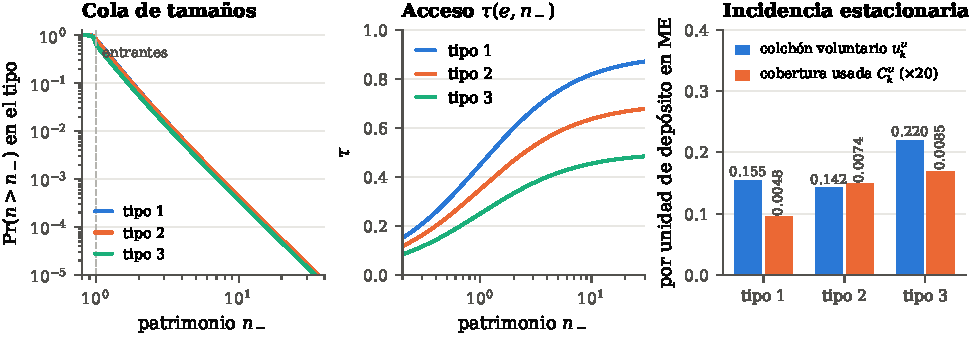
\includegraphics[width=\textwidth]{fig09_bancos_estado_estacionario.pdf}
\caption{Estado estacionario del prototipo. Izquierda: cola de la distribución de
tamaños dentro de cada tipo; la mediana está en $1.13$ y el percentil 99 en
$3.60$ veces el tamaño de entrada. Centro: el acceso al interbancario crece con
el tamaño, lo que hace que la distribución importe para los agregados. Derecha:
la incidencia estacionaria por tipo.}
\label{fig:bancos-ss}
\end{figure}

El panel derecho de la figura \ref{fig:bancos-ss} contiene el resultado
distributivo básico, que reproduce la hipótesis del marco estático y la matiza:

\begin{itemize}[leftmargin=1.4em]
\item El tipo más expuesto y con peor acceso (tipo 3) utiliza un $78\%$ más de
cobertura pública por unidad de depósito en moneda extranjera que el tipo menos
expuesto ($0.0085$ frente a $0.0048$).
\item Pero también mantiene el mayor colchón voluntario ($22.0\%$ frente a
$15.5\%$). El autoseguro \emph{atenúa} el ordenamiento sin revertirlo, que es
exactamente la salvedad que el marco estático anticipa.
\item Hay una no monotonicidad que vale la pena notar: el tipo 2 mantiene
\emph{menos} colchón que el tipo 1 ($14.2\%$ frente a $15.5\%$) pese a ser más
expuesto. La razón es que el colchón cubre dos riesgos distintos ---
el idiosincrático y el agregado --- y para un banco de baja dispersión
el motivo agregado domina y no escala con $a_e$. Es un mecanismo que el modelo
estático con un solo choque no puede generar.
\end{itemize}

\section{Los jacobianos del bloque}

\begin{figure}[htbp]
\centering
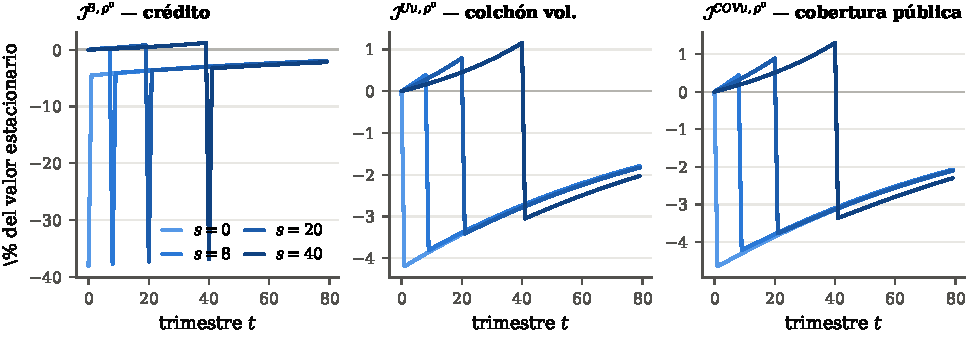
\includegraphics[width=\textwidth]{fig10_bancos_jacobianos.pdf}
\caption{Columnas del jacobiano del bloque bancario respecto del encaje exigible
en moneda extranjera. Cada curva es la respuesta a la noticia, recibida hoy, de
que $\rho^u$ será un punto más alto en la fecha $s$.}
\label{fig:bancos-J}
\end{figure}

Hay dos verificaciones analíticas que estos jacobianos pasan exactamente y que
conviene usar siempre que se construye un bloque nuevo.

\begin{enumerate}[leftmargin=1.4em]
\item $\J^{B,\rho^u}_{0,0} = -3.265699$, que coincide hasta la última cifra con
$-D^u_\sst = -3.265699$. Tiene que ser así: un punto más de encaje inmoviliza
exactamente un punto de los depósitos en moneda extranjera, y en impacto los
depósitos están predeterminados.
\item $\J^{Y,\rho^u}_{0,s} = 0$ para todo $s\ge1$ y toda variable de acervo $Y$.
Una noticia sobre el encaje futuro no puede cambiar el crédito ni el patrimonio
de hoy, porque ambos están determinados por la distribución heredada. Lo que
\emph{sí} cambia hoy es el dividendo --- el banco retiene más capital anticipando
el costo futuro --- y en efecto $\J^{\mathrm{div},\rho^u}_{0,5} = -7.8\times10^{-4}$.
\end{enumerate}

\begin{idea}
Esa pareja de verificaciones es el mejor ejemplo de lo que un jacobiano enseña.
La primera fila de la matriz dice qué puede moverse hoy: solo las variables de
flujo que son elección. Todo lo demás es acervo heredado. Si tu código produce
una respuesta no nula en la primera fila para una variable predeterminada, hay un
error de contabilidad temporal.
\end{idea}

\section{Un choque de encaje: el canal que el modelo estático no ve}

La figura \ref{fig:bancos-irf} muestra la respuesta de equilibrio general a un
aumento de un punto porcentual del encaje en moneda extranjera, con persistencia
AR(1) de $0.90$.

\begin{figure}[htbp]
\centering
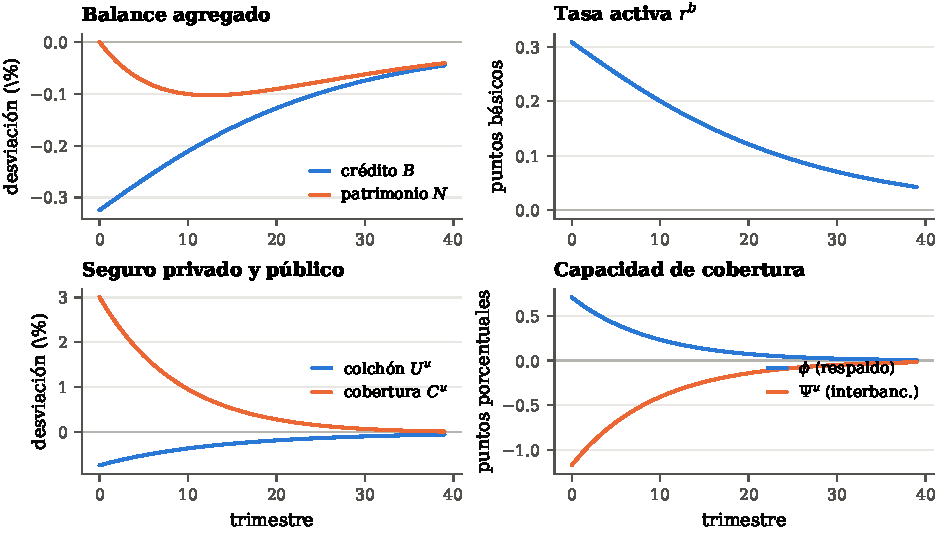
\includegraphics[width=\textwidth]{fig11_bancos_irf_encaje.pdf}
\caption{Respuesta a un aumento de 1 punto porcentual del encaje exigible en
moneda extranjera ($\rho=0.90$). El patrimonio está predeterminado en impacto y
se erosiona después; el colchón voluntario \emph{cae}; la cobertura pública
utilizada \emph{sube}.}
\label{fig:bancos-irf}
\end{figure}

Los números en impacto: el crédito cae $0.32\%$, la tasa activa sube $0.31$
puntos básicos, el colchón voluntario en moneda extranjera cae $0.74\%$ y la
cobertura pública utilizada sube $3.00\%$. El patrimonio no se mueve en impacto
--- está predeterminado --- y alcanza su caída máxima de $0.10\%$ en el trimestre
12.

El resultado interesante es el del colchón voluntario, y conviene entender por
qué ocurre. Estamos en régimen de \emph{encaje no utilizable}: el requisito no
es un colchón, de modo que $\partial u^u/\partial\rho^u = 0$ \emph{dentro del
bloque} --- en efecto, $\J^{Uu,\rho^u}_{0,0}=0$ exactamente. Sin embargo, en
equilibrio general el colchón cae. El canal es indirecto:

\begin{equation}
\rho^u \uparrow
\;\Longrightarrow\;
F^u = v_F\rho^u D^u \uparrow
\;\Longrightarrow\;
\phi = \min(1, F^u/\Delta^u) \uparrow
\;\Longrightarrow\;
\iota^{\text{ef}} = \phi\iota^u + (1-\phi)\bar\iota^u \downarrow
\;\Longrightarrow\;
u^u \downarrow .
\end{equation}

Es decir: \textbf{el encaje desplaza liquidez voluntaria no porque la sustituya
mecánicamente, sino porque engorda el fondo de respaldo y abarata el faltante}.
En impacto $\phi$ sube $0.88\%$ y eso basta para que el colchón caiga $0.74\%$ y
la cobertura utilizada suba $3.00\%$. Este canal no existe en el modelo
estático con $\phi$ dado, y es el tipo de resultado que justifica el esfuerzo de
pasar a dinámico.

\paragraph{Incidencia} El panel izquierdo de la figura \ref{fig:bancos-incid}
muestra que el aumento relativo de la cobertura utilizada es mayor para el tipo
menos expuesto ($+3.97\%$) que para los tipos 2 y 3 ($+2.53\%$ y $+2.75\%$).
Conviene no leer mal este resultado: en \emph{niveles} el tipo 3 sigue usando
mucha más cobertura, porque parte de una base casi el doble de grande. Lo que
dice el ejercicio es que el ajuste marginal ante un cambio de encaje recae
proporcionalmente más sobre los bancos menos expuestos. Separar la incidencia
en niveles de la incidencia marginal es, probablemente, una distinción que vale
la pena hacer explícita en una tesis sobre incidencia.

\begin{figure}[htbp]
\centering
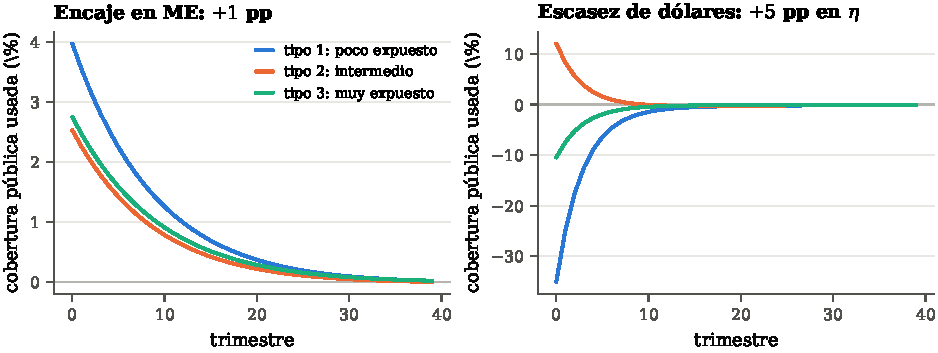
\includegraphics[width=\textwidth]{fig12_bancos_incidencia.pdf}
\caption{Respuesta de la cobertura pública utilizada por tipo de banco, en
porcentaje de su valor estacionario. Izquierda: choque de encaje. Derecha:
choque de escasez de dólares. El cambio de signo entre tipos en el panel derecho
es un mecanismo del modelo, no un artefacto numérico; se explica en el texto.}
\label{fig:bancos-incid}
\end{figure}

\section{Un choque de escasez de dólares}

El panel derecho de la figura \ref{fig:bancos-incid} muestra algo más llamativo.
Ante un aumento de 5 puntos porcentuales en la magnitud de la salida agregada de
dólares, la cobertura utilizada por el tipo 1 \emph{cae} un $35\%$, la del tipo 2
\emph{sube} un $12\%$ y la del tipo 3 cae un $10\%$.

El mecanismo es el siguiente, y vale la pena seguirlo porque ilustra cómo se
diagnostica un resultado contraintuitivo.

\begin{enumerate}[leftmargin=1.4em]
\item Para el tipo 1, cuya dispersión idiosincrática es pequeña ($a=0.08$), el
colchón óptimo está determinado \emph{solo} por el motivo agregado: en el estado
normal su posición de liquidez ya excede $a$ y nunca tiene faltante. La derivada
numérica confirma $\partial u^u/\partial\eta = 1.0000$ exactamente: ese banco
compensa la salida agregada uno a uno.
\item Los tipos 2 y 3 también se aseguran contra el riesgo idiosincrático, de
modo que su colchón responde solo parcialmente: $\partial u^u/\partial\eta$ vale
$0.32$ y $0.30$.
\item En equilibrio general, el choque reduce la holgura del interbancario
($-11.4\%$) y la capacidad de respaldo ($-6.8\%$), lo que encarece el faltante
residual y empuja a todos los bancos a aumentar su colchón más allá de la
compensación mecánica. El colchón agregado sube $25.8\%$.
\item Para el tipo 1, ese exceso de autoseguro domina: su posición de liquidez
esperada \emph{mejora}, su faltante esperado cae y termina usando menos
cobertura pública. Para el tipo 2 no alcanza y termina usando más.
\end{enumerate}

\begin{idea}
La lectura económica es que un choque de escasez de dólares provoca una
\emph{huida hacia el autoseguro privado}, y que esa huida es más intensa
--- en términos relativos --- entre los bancos cuyo único motivo de liquidez es
el riesgo agregado. El resultado es una recomposición de quién usa el respaldo
público, no solo un cambio de nivel. Es exactamente la clase de pregunta
distributiva que motiva el marco estático, y solo el modelo dinámico con
equilibrio general simultáneo la puede contestar.
\end{idea}

\section{Encaje utilizable y el umbral}
\label{sec:regimenes}

El marco estático menciona, como resultado secundario, que bajo \emph{encaje
utilizable} un aumento del requisito podría sustituir liquidez voluntaria. El
prototipo lo hace preciso.

\begin{figure}[htbp]
\centering
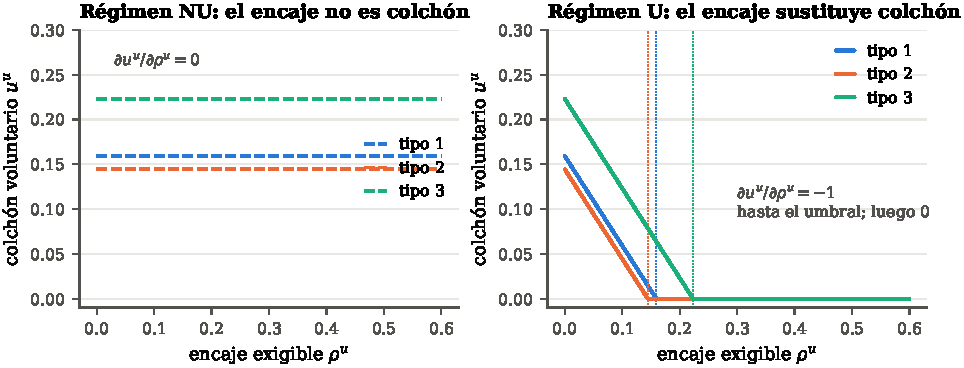
\includegraphics[width=\textwidth]{fig13_bancos_regimenes.pdf}
\caption{Colchón voluntario óptimo en función del encaje exigible, por tipo de
banco. Bajo encaje no utilizable (izquierda) el requisito no afecta la decisión
privada. Bajo encaje utilizable (derecha) la sustituye uno a uno hasta un umbral
--- el nivel que el banco elegiría por sí mismo --- y después deja de tener
efecto marginal.}
\label{fig:regimenes}
\end{figure}

Bajo encaje utilizable, el colchón efectivo es $\mu^c = \max\{\rho^c, \mu^{c*}\}$,
donde $\mu^{c*}$ resuelve \eqref{eq:cpo}. Por lo tanto
\begin{equation}
u^c = \max\{\mu^{c*}-\rho^c,\,0\},
\qquad
\frac{\partial u^c}{\partial \rho^c} =
\begin{cases}
-1 & \text{si } \rho^c < \mu^{c*} \quad\text{(sustitución uno a uno)}\\
0 & \text{si } \rho^c > \mu^{c*} \quad\text{(el requisito es holgado)}
\end{cases}
\end{equation}

El umbral $\mu^{c*}$ depende del tipo: en la calibración vale $0.159$, $0.144$ y
$0.223$ para los tres tipos. Con un encaje exigible en moneda extranjera de
$35.4\%$, los tres están muy por encima de su umbral, de modo que bajo encaje
utilizable el requisito eliminaría prácticamente todo el riesgo de liquidez en
dólares --- y con él, el motivo asegurador que el marco estático quiere estudiar.

\begin{tutesis}
Esto es un resultado con consecuencias directas para tu diseño de investigación,
y conviene tenerlo claro antes de IE2. La distinción entre encaje utilizable y
no utilizable no es un detalle de implementación: determina si el instrumento
\emph{tiene} un margen interesante. Con $\rho^u=35\%$ y choques de retiro de
hasta $28\%$ de los depósitos, bajo encaje utilizable no hay faltante en casi
ningún estado y el modelo se vuelve degenerado. Tu interpretación del encaje
como un \emph{fondo} que financia un seguro --- es decir, el régimen NU --- no es
solo la más fiel al arreglo institucional peruano: es la única bajo la cual la
pregunta de incidencia tiene contenido con encajes de esa magnitud. Vale la pena
decirlo así, con el número al lado, en lugar de presentar NU como un supuesto
auxiliar.
\end{tutesis}

\section{Qué habría que arreglar antes de usar esto cuantitativamente}
\label{sec:limitaciones-prototipo}

El prototipo es correcto como ilustración del método y es honesto decir dónde no
alcanza.

\begin{enumerate}[leftmargin=1.4em]
\item \textbf{La fricción de pago de dividendos es una forma reducida.} La
utilidad cóncava sobre dividendos es un sustituto conveniente de un costo de
emisión de capital o de un valor de franquicia, pero no está microfundada y sus
parámetros no están disciplinados por nada. Para un ejercicio cuantitativo
convendría reemplazarla por una especificación tipo Gertler--Karadi con una
restricción de incentivos explícita.
\item \textbf{La restricción de apalancamiento es exógena y siempre ata.} En los
datos el ratio de capital varía por banco y en el tiempo, y a veces no ata.
\item \textbf{Los choques en soles y en dólares son independientes.} En una
crisis de dolarización están correlacionados, y esa correlación es probablemente
importante para la demanda de cobertura conjunta.
\item \textbf{La composición monetaria $w_e$ es fija.} El marco estático lo
justifica como aproximación de primer orden, y es razonable; pero en un modelo
dinámico la sustitución de depósitos entre monedas ante un cambio de encaje es un
canal de política de primer orden.
\item \textbf{No hay precio del dólar.} Un modelo que quiera hablar de escasez de
dólares en serio necesita un tipo de cambio y una condición de arbitraje.
\item \textbf{La calibración es ilustrativa.} Las dispersiones $a_e$ están
elegidas para abarcar el rango observado de volatilidad de depósitos, no
estimadas; $\tau_e$, $\iota^u$ y $\bar\iota^u$ no están disciplinados por nada.
El capítulo \ref{cap:hoja-ruta} propone cómo disciplinarlos.
\end{enumerate}

Ninguna de estas limitaciones es del método: todas son del modelo. Esa distinción
importa, porque significa que arreglarlas no obliga a cambiar de herramienta.

\chapter{Hoja de ruta de implementación}
\label{cap:hoja-ruta}

Este capítulo propone un orden de trabajo. Está pensado para alguien que tiene un
modelo estático funcionando y un semestre por delante. Cada etapa termina con un
criterio verificable: si no se cumple, no conviene pasar a la siguiente.

\section{Etapa 0: el estado estacionario del modelo que ya tienes}

\paragraph{Qué hacer} Escribir en código el modelo estático que ya existe, pero
estructurado como el estado estacionario de un modelo dinámico: una función que,
dados los parámetros y los precios, devuelva todas las cantidades agregadas.

\paragraph{Criterio de salida} El código reproduce exactamente los números del
modelo estático escrito en papel, y las identidades contables (el balance de cada
banco, la identidad $X-G=\mu$, la suma de masas igual a uno) se cumplen a
precisión de máquina.

\paragraph{Cuánto toma} Una o dos semanas. Es tiempo bien gastado: el 80\% de los
errores que aparecerían después se atrapan aquí.

\section{Etapa 1: cerrar las decisiones pendientes}

\paragraph{Qué hacer} Convertir en decisiones todo lo que ahora es parámetro
impuesto. En el modelo de la parte V, eso significa derivar la liquidez
voluntaria de una condición de primer orden en lugar de fijarla. Para cada
decisión que se cierre, hay que escribir explícitamente el problema de
optimización, su condición de primer orden, y verificar numéricamente que la
solución la satisface.

\paragraph{Criterio de salida} Ninguna variable de elección es un parámetro
libre, y para cada una se puede decir qué fuerzas económicas la determinan y en
qué dirección responde a cada precio.

\section{Etapa 2: añadir el estado endógeno individual}

\paragraph{Qué hacer} Introducir el estado que acumula --- el patrimonio, en el
caso bancario --- con su ley de movimiento y su problema dinámico. Resolver el
estado estacionario completo: iteración hacia atrás, distribución estacionaria,
agregación.

\paragraph{Criterio de salida}
\begin{enumerate}[leftmargin=1.4em,itemsep=1pt]
\item La distribución converge a $10^{-14}$ y suma uno.
\item La masa en el último punto de la grilla es despreciable (digamos, menor
que $10^{-8}$). Si no, la grilla está atando y hay que extenderla o revisar la
condición de crecimiento.
\item El modelo reproduce la versión sin estado endógeno cuando se apaga el
mecanismo que lo hace relevante.
\item Las magnitudes agregadas son plausibles: ratio de capital, rentabilidad,
apalancamiento.
\end{enumerate}

\paragraph{Cuánto toma} Dos a cuatro semanas. Es la etapa con más trabajo
conceptual nuevo.

\section{Etapa 3: los jacobianos del bloque}

\paragraph{Qué hacer} Implementar el algoritmo fake news para el bloque, y
verificarlo.

\paragraph{Criterio de salida} \emph{Este es el criterio innegociable del
proyecto.} El jacobiano calculado con el algoritmo rápido coincide con el del
método directo, a $T=30$ o $40$, con error relativo menor que $10^{-6}$ en
\emph{todos} los pares insumo--producto. Además, todas las identidades
analíticas que el modelo implique se verifican.

\begin{trampa}
La tentación de saltarse la verificación contra el método directo es enorme,
porque el algoritmo rápido ``parece funcionar'': produce matrices con la forma
correcta y signos razonables. Casi todos los errores de implementación de este
método --- el orden invertido de los operadores, un índice desfasado en la
recursión, una distribución mal alineada --- producen jacobianos que se ven bien
y están mal. Escribir el método directo cuesta veinte líneas y es la única
defensa real.
\end{trampa}

\section{Etapa 4: el equilibrio general}

\paragraph{Qué hacer} Armar el grafo, elegir incógnitas y objetivos, resolver.

\paragraph{Criterio de salida}
\begin{enumerate}[leftmargin=1.4em,itemsep=1pt]
\item El número de condición de $\mathbf{H}_U$ es razonable.
\item Las respuestas en impacto de las variables predeterminadas son cero.
\item La condición de vaciado omitida por la ley de Walras da residuo numérico
nulo.
\item La solución no cambia al pasar de $T$ a $1.5T$.
\end{enumerate}

\section{Etapa 5: disciplinar la calibración}

Aquí es donde el proyecto deja de ser un ejercicio y empieza a decir algo. La
pregunta que organiza esta etapa es: \emph{¿qué dato identifica a qué parámetro?}

La tabla \ref{tab:identificacion} es un ejemplo de cómo organizarla para el
modelo bancario de la parte V. El punto no son las entradas concretas sino el
ejercicio: para cada parámetro, un momento, y para cada momento, una razón por la
que es informativo sobre ese parámetro y no sobre otro.

\begin{table}[htbp]
\centering\small\setlength{\tabcolsep}{4pt}
\caption{Qué dato disciplina a qué parámetro en el modelo bancario.}
\label{tab:identificacion}
\begin{tabular}{@{}p{0.19\textwidth}p{0.33\textwidth}p{0.40\textwidth}@{}}
\toprule
\textbf{Parámetro} & \textbf{Momento} & \textbf{Por qué es informativo}\\
\midrule
$a_e$ (exposición) & volatilidad del crecimiento de depósitos, por banco &
es directamente la dispersión del choque de retiro, en el corte transversal\\
$\tau_e$ (acceso) & saldos interbancarios sobre activos, por banco &
un banco con mejor acceso opera más en el mercado\\
$w_e$ (dolarización) & participación de depósitos en ME, por banco &
observable directamente\\
$\lambda$ (apalancamiento) & ratio de capital del sistema & contable\\
$\eta$, $p$ (estado agregado) & frecuencia y magnitud de episodios de salida de
depósitos en ME & serie agregada\\
$v_F$, $\bar\iota^u$ (respaldo) & uso de las operaciones de liquidez del banco
central en episodios de tensión & es la variable que el modelo llama $C^u$\\
$\beta$, $\varsigma$ (banquero) & rentabilidad y tasa de salida de bancos &
fijan el crecimiento y la escala\\
\bottomrule
\end{tabular}
\end{table}

\begin{idea}
Nótese que casi todos los momentos de la tabla son \emph{transversales}, no de
series de tiempo. Eso no es casualidad: la heterogeneidad se identifica con
variación entre unidades. Una estrategia de calibración que solo use agregados no
puede separar parámetros que afectan a los agregados de la misma forma, como se
advirtió en el capítulo \ref{cap:estimacion}.
\end{idea}

\section{Etapa 6: los ejercicios que valen la pena}

Una vez que el modelo funciona, estos son los ejercicios que un modelo dinámico
puede hacer y uno estático no. Están ordenados por relación entre valor y
esfuerzo.

\begin{enumerate}[leftmargin=1.4em]
\item \textbf{Respuesta a un cambio de encaje, anticipado y no anticipado.}
Comparar la columna $s=0$ con la columna $s=8$ del jacobiano de equilibrio
general. Esto responde directamente a una pregunta de diseño de política: ¿sirve
anunciar con antelación?
\item \textbf{Incidencia dinámica por tipo.} Cómo se reparte el ajuste entre
clases de banco, y cómo cambia ese reparto a lo largo de la transición.
\item \textbf{Erosión del capital.} Cuánto del efecto de largo plazo de una
política viene del canal de acumulación y cuánto del efecto contemporáneo. Se
mide apagando el estado endógeno.
\item \textbf{Transición entre regímenes de encaje.} Usar el método del capítulo
\ref{cap:nolineal} para calcular la trayectoria completa de una reforma
permanente.
\item \textbf{A qué tamaño de choque se rompe la linealidad.} Encontrar el
choque de escasez que agota la capacidad de respaldo, y mostrar cuánto se separa
la respuesta no lineal de la lineal en ese punto.
\end{enumerate}

\section{Qué hacer si el tiempo se acaba}

Un plan realista tiene que contemplar que no todo entre. Si hay que recortar, el
orden de prioridad sugerido es:

\begin{itemize}[leftmargin=1.4em]
\item \textbf{Conservar siempre:} la etapa 3 completa, con su verificación. Un
jacobiano verificado es un resultado defendible aunque no haya equilibrio general.
\item \textbf{Recortar primero:} la estimación. Calibrar es perfectamente
defendible en una tesis de pregrado, y la estimación bayesiana agrega mucho
riesgo por poco contenido adicional.
\item \textbf{Recortar segundo:} las transiciones no lineales. Son valiosas pero
son un complemento.
\item \textbf{Simplificar antes de abandonar:} si el modelo completo con dos
monedas y tres tipos no converge a tiempo, un modelo con una moneda y dos tipos
que \emph{funciona y está verificado} vale infinitamente más que uno completo que
no corre.
\end{itemize}


\appendix
\part*{Apéndices}
\addcontentsline{toc}{part}{Apéndices}
\chapter{El código}
\label{ap:codigo}

Todo el material numérico de este manual se produjo con una implementación
propia, escrita desde cero y sin dependencias más allá de \texttt{numpy},
\texttt{scipy} y \texttt{matplotlib}. La prioridad fue la legibilidad: el código
está pensado para leerse junto con los capítulos \ref{cap:bloque} a
\ref{cap:dag}.

\section{Estructura}

\begin{center}\small
\begin{tabular}{@{}lp{0.62\textwidth}@{}}
\toprule
\texttt{ssj/grids.py} & grillas y discretización de Rouwenhorst\\
\texttt{ssj/interpolate.py} & interpolación, lotería de Young, pasos hacia
adelante y de expectativa\\
\texttt{ssj/het.py} & el bloque heterogéneo y el algoritmo fake news\\
\texttt{ssj/simple.py} & bloques simples, grafo acíclico, solución de equilibrio\\
\texttt{models/krusell\_smith.py} & el modelo de referencia\\
\texttt{models/banks.py} & el bloque bancario de la parte V\\
\texttt{models/banks\_ge.py} & su equilibrio general\\
\texttt{tests/test\_fakenews.py} & verificación contra el método directo\\
\texttt{figures/} & generación de todas las figuras\\
\bottomrule
\end{tabular}
\end{center}

\section{Cómo correrlo}

\begin{lstlisting}[language=bash,numbers=none,basicstyle=\ttfamily\footnotesize]
pip install numpy scipy matplotlib
cd code
python3 tests/test_fakenews.py     # verificacion (deberia decir TODO OK)
python3 figures/fig_metodo.py      # figuras 1 a 8
python3 figures/fig_bancos.py      # figuras 9 a 13
\end{lstlisting}

La verificación tarda unos segundos; las figuras del modelo bancario tardan unos
minutos la primera vez, porque resuelven el punto fijo del estado estacionario, y
después usan un caché en disco.

\section{El núcleo del algoritmo}

Vale la pena leer estas treinta líneas con la receta del capítulo
\ref{cap:fakenews} al lado. Son la traducción literal de los cuatro pasos.

\paragraph{Paso 1: una sola iteración hacia atrás}

\begin{lstlisting}
def _backward_fakenews(self, ss, shocked, T, h):
    """Una sola iteracion hacia atras entrega TODAS las columnas."""
    base = {k: ss[k] for k in self.inputs}
    curlyY = {o: np.empty((2, T)) for o in self.outputs}
    curlyD = np.empty((2, T, self.ne, self.na))

    for sgn_idx, sgn in enumerate((+1.0, -1.0)):   # diferenciacion de dos lados
        V_next = ss["V"]
        for s in range(T):
            args = dict(base)
            if s == 0:
                args[shocked] = base[shocked] + sgn * h
            V_next, pol, out = self._step(V_next, **args)
            for o in self.outputs:
                curlyY[o][sgn_idx, s] = np.vdot(out[o], ss["D"])   # dY_0^s
            i, p = lottery(pol, self.grid)
            curlyD[sgn_idx, s] = self._forward(ss["D"], i, p)      # dD_1^s

    dY = {o: (curlyY[o][0] - curlyY[o][1]) / (2 * h) for o in self.outputs}
    dD = (curlyD[0] - curlyD[1]) / (2 * h)
    return dY, dD
\end{lstlisting}

El punto que hay que ver: el bucle sobre \texttt{s} no reinicia nada. La
variable \texttt{V\_next} se arrastra de una iteración a la siguiente, de modo
que en la iteración $s$ la función de continuación ya incorpora el efecto de un
choque que ocurre $s$ períodos en el futuro. Eso es el lema
\ref{lema:politicas} hecho código.

\paragraph{Pasos 2 a 4: expectativas, matriz $\F$ y acumulación}

\begin{lstlisting}
def _expectations(self, ss, T):
    """E_t = Lambda^t y_ss: T-1 aplicaciones de una matriz fija."""
    curlyE = {}
    for o in self.outputs:
        E = np.empty((T - 1, self.ne, self.na))
        E[0] = ss["outcomes"][o]
        for t in range(1, T - 1):
            E[t] = self._expect(E[t - 1], ss["i"], ss["p"])
        curlyE[o] = E
    return curlyE

def jacobians(self, ss, shocked_inputs=None, T=300, h=1e-4, return_F=False):
    shocked_inputs = shocked_inputs or self.inputs
    curlyE = self._expectations(ss, T)                       # paso 2
    dY, dD = {}, {}
    for i in shocked_inputs:
        dY[i], dD[i] = self._backward_fakenews(ss, i, T, h)  # paso 1

    Fs, Js = {}, {}
    for o in self.outputs:
        Emat = curlyE[o].reshape(T - 1, -1)
        for i in shocked_inputs:
            F = np.empty((T, T))                             # paso 3
            F[0, :] = dY[i][o]
            F[1:, :] = Emat @ dD[i].reshape(T, -1).T
            Fs[(o, i)] = F
            J = F.copy()                                     # paso 4
            for t in range(1, T):
                J[t, 1:] += J[t - 1, :-1]
            Js[(o, i)] = J
    return (Js, Fs) if return_F else Js
\end{lstlisting}

El paso 3 es una sola multiplicación de matrices de $(T-1)\times n_g$ por
$n_g\times T$, y el paso 4 es una recursión de $T$ líneas sobre una matriz
$T\times T$. Ahí está todo el algoritmo.

\section{Los dos operadores que hay que no confundir}

\begin{lstlisting}
def forward_step(D, Pi, i, p):
    """D_{t+1} = Lambda' D_t: primero la loteria, luego Markov exogeno."""
    return Pi.T @ forward_policy(D, i, p)

def expectation_step(E, Pi, i, p):
    """E_t = Lambda E_{t-1}: primero Markov exogeno, luego la loteria.

    Notese el orden INVERSO. Es la transpuesta del mismo operador: si
    Lambda' = Pi' L'  entonces  Lambda = L Pi. Confundir este orden produce
    jacobianos casi correctos, y diagnosticarlo cuesta horas.
    """
    Etilde = Pi @ E
    out = np.empty_like(E)
    for e in range(E.shape[0]):
        out[e] = p[e] * Etilde[e, i[e]] + (1 - p[e]) * Etilde[e, i[e] + 1]
    return out
\end{lstlisting}

\section{La verificación}

\begin{lstlisting}
def test_budget_and_signs():
    het = make_household(n_a=100, amax=150)
    ss = household_ss(het, r=0.01, w=1.0, eis=0.5, target_A=3.0)
    J = het.jacobians(ss, ["r", "w"], T=30)

    # restriccion presupuestaria agregada en la fecha 0:
    #   dC_0 + dA_0 = dw_0 * E[e]
    lhs = J[("C", "w")][0, 0] + J[("A", "w")][0, 0]
    assert abs(lhs - 1.0) < 1e-5

    # una NOTICIA sobre el futuro no cambia los recursos de hoy:
    #   dC_0 + dA_0 = 0  para s >= 1
    for s in (1, 5, 10):
        assert abs(J[("C", "w")][0, s] + J[("A", "w")][0, s]) < 1e-6
\end{lstlisting}

Esta prueba no mira ninguna magnitud económica: solo verifica contabilidad. Por
eso es tan útil. Un error de alineación temporal, de orden de operadores o de
índices rompe la contabilidad mucho antes de volver implausible el resultado
económico.

\section{Resultados de la verificación}

Al correr \texttt{tests/test\_fakenews.py} sobre el bloque de hogares de
Krusell--Smith con $T=40$ y 100 puntos de activos:

\begin{center}\small
\begin{tabular}{@{}lrr@{}}
\toprule
& \textbf{error absoluto} & \textbf{error relativo}\\
\midrule
$\J^{A,r}$ & $3.3\times10^{-8}$ & $5.5\times10^{-9}$\\
$\J^{A,w}$ & $1.5\times10^{-8}$ & $1.7\times10^{-8}$\\
$\J^{C,r}$ & $1.2\times10^{-9}$ & $3.6\times10^{-9}$\\
$\J^{C,w}$ & $1.4\times10^{-8}$ & $9.7\times10^{-8}$\\
\bottomrule
\end{tabular}
\end{center}

Y sobre el bloque bancario de la parte V, con 78 pares insumo--producto, el peor
error relativo es $2.9\times10^{-8}$.

\chapter{Ejercicios}
\label{ap:ejercicios}

Los ejercicios están ordenados por dificultad. Los marcados con $\star$ requieren
código; los demás son de lápiz. Las soluciones de los primeros están al final.

\section{Entender el objeto}

\paragraph{B.1} Un consumidor con utilidad logarítmica, horizonte infinito y
$\beta(1+r)=1$ tiene el jacobiano $\J^{C,y}_{t,s} = \frac{r}{1+r}(1+r)^{-s}$ de
la ecuación \eqref{eq:jac-ri}. (a) Verifica que todas las filas son iguales.
(b) ¿Cuánto suma cada fila cuando $T\to\infty$, y qué significa económicamente?
(c) Dibuja cómo cambiaría la matriz si el agente estuviera restringido en
liquidez.

\paragraph{B.2} Explica, sin fórmulas, por qué la primera fila del jacobiano de
una variable de acervo tiene ceros en todas las columnas $s\ge1$. Da un ejemplo
de una variable del mismo modelo cuya primera fila \emph{no} tenga ceros ahí.

\paragraph{B.3} El jacobiano de un bloque es triangular inferior. ¿Qué dice eso
sobre el comportamiento de los agentes del bloque? Si ese bloque modela hogares
que optimizan, ¿es un resultado o un error?

\section{El algoritmo}

\paragraph{B.4} Usando la proposición \ref{prop:principal}, escribe $\J_{3,2}$
como suma de entradas de $\F$. Verifica que la cantidad de términos coincide con
$\min\{s,t\}+1$.

\paragraph{B.5} El lema \ref{lema:politicas} vale sin aproximación; el lema
\ref{lema:fake} requiere $dx$ infinitesimal. ¿En qué paso exacto de la
demostración del lema \ref{lema:fake} se usa que el choque es infinitesimal?

\paragraph{B.6} Supón que $D_0 \neq D_\sst$. ¿Qué parte de la proposición
\ref{prop:principal} se rompe? ¿Por qué el método sigue sirviendo para calcular
transiciones desde una distribución arbitraria (capítulo \ref{cap:nolineal})?

\paragraph{B.7 $\star$} En el código, cambia el orden de los operadores en
\texttt{expectation\_step} (aplica primero la lotería y después $\Pi$). Calcula
los jacobianos y compáralos con el método directo. ¿Cuánto cambian? ¿Lo habrías
notado mirando solo la figura?

\section{Equilibrio general}

\paragraph{B.8} En el modelo de Krusell--Smith del capítulo \ref{cap:dag}, ¿por
qué $r$ y $w$ no son incógnitas? ¿Qué pasaría con el tamaño del sistema si lo
fueran?

\paragraph{B.9} Un modelo tiene tres bloques con un ciclo: $b_1\to b_2 \to b_3
\to b_1$. Describe cómo convertirlo en acíclico, y cuántas incógnitas y objetivos
nuevos hacen falta.

\paragraph{B.10 $\star$} Resuelve el modelo de Krusell--Smith con $T=50$ y con
$T=300$ para un choque AR(1) con $\rho=0.99$. Compara las respuestas en los
primeros 20 trimestres. Explica la diferencia.

\section{Macrofinanzas}

\paragraph{B.11} Demuestra la identidad $X(\mu;a) - G(\mu;a) = \mu$ usada en el
capítulo \ref{cap:aplicacion}, donde $X=\Ex[(\varepsilon+\mu)^+]$ y
$G=\Ex[(-(\varepsilon+\mu))^+]$ con $\Ex[\varepsilon]=0$. ¿Por qué es útil como
prueba del código?

\paragraph{B.12} Con $\varepsilon\sim U[-a,a]$, deriva \eqref{eq:G} integrando
directamente. Verifica que $G$ es continua y derivable en $\mu=\pm a$, y que
$G'$ \emph{no} es derivable ahí. ¿Importa para el método?

\paragraph{B.13} En el régimen de encaje utilizable, el colchón voluntario es
$u = \max\{\mu^*-\rho, 0\}$. Calcula $\partial u/\partial\rho$ a cada lado del
umbral. ¿Qué pasa con el jacobiano agregado si distintos bancos tienen umbrales
distintos?

\paragraph{B.14} Explica por qué, en un modelo bancario con retornos exactamente
lineales en el patrimonio y sin costos fijos, la distribución de tamaños no
afecta a ningún agregado. Propón tres modificaciones que rompan esa propiedad y
di cuál te parece más defendible empíricamente.

\paragraph{B.15 $\star$} En el modelo bancario, calcula $\partial u^u/\partial\eta$
por tipo con diferenciación numérica directa sobre la condición de primer orden.
Verifica que vale exactamente $1$ para el tipo de menor dispersión y explica por
qué.

\section{Soluciones seleccionadas}

\paragraph{B.1} (a) Porque $\partial c_t/\partial y_s$ no depende de $t$: el
agente consume la anualidad de la riqueza, y la fecha en que llega el ingreso solo
afecta su valor presente, no el perfil de consumo. (b) Cada fila suma
$\frac{r}{1+r}\sum_s (1+r)^{-s} = \frac{r}{1+r}\cdot\frac{1+r}{r} = 1$: un sol
adicional de valor presente se consume íntegramente, repartido en el tiempo.
(c) La diagonal se vuelve mucho mayor y las entradas lejanas caen: el agente
restringido consume hoy lo que recibe hoy y no puede adelantar ingreso futuro.

\paragraph{B.2} Porque un acervo en la fecha $0$ está determinado por la
distribución heredada $D_0=D_\sst$ y por los insumos de la fecha $0$; una noticia
sobre $s\ge1$ no puede alterar ninguno de los dos. Un ejemplo de variable cuya
primera fila sí es distinta de cero: cualquier \emph{flujo} de elección ---
consumo, dividendos, el colchón voluntario --- que el agente ajusta hoy
anticipando el futuro.

\paragraph{B.3} Dice que los agentes no son prospectivos: su decisión en $t$ no
responde a nada posterior a $t$. Si el bloque modela agentes que optimizan con
expectativas, es un error: casi seguro la iteración hacia atrás no está
propagando la variable de continuación.

\paragraph{B.4} $\J_{3,2} = \F_{3,2} + \F_{2,1} + \F_{1,0}$, que son
$\min\{2,3\}+1 = 3$ términos.

\paragraph{B.5} En el paso donde se linealiza \eqref{eq:canon-Y} y
\eqref{eq:canon-D}, es decir al escribir $dY^s_t = y_\sst'dD^s_t + (dy^s_t)'D_\sst$
y $dD^s_t = \Lambda_\sst' dD^s_{t-1} + (d\Lambda^s_{t-1})'D_\sst$. Ambas son
expansiones de primer orden: con $dx$ finito habría términos cruzados
$(dy^s_t)'dD^s_t$ que no se cancelan.

\paragraph{B.6} Se rompe el último paso de la demostración del lema
\ref{lema:fake}, donde se usa $dD^{s-1}_0=0$ para cerrar la recursión. El método
del capítulo \ref{cap:nolineal} sigue sirviendo porque ahí los jacobianos se usan
solo como \emph{aproximación del jacobiano verdadero} en una iteración de
cuasi-Newton: el sistema que se resuelve es el no lineal exacto, y la calidad de
la aproximación solo afecta la velocidad de convergencia, no el punto al que se
converge.

\paragraph{B.8} Porque las condiciones de primer orden de la empresa permiten
despejarlos explícitamente en función de $K_{t-1}$ y $Z_t$. Si fueran incógnitas,
el sistema pasaría de $300\times300$ a $900\times900$ y la inversión costaría
unas 27 veces más, sin ganar nada.

\paragraph{B.11} $X - G = \Ex[(\varepsilon+\mu)^+] - \Ex[(-(\varepsilon+\mu))^+]
= \Ex[(\varepsilon+\mu)] = \mu$, usando $z^+ - (-z)^+ = z$ para todo $z$ real.
Es útil porque se cumple para \emph{cualquier} distribución con media cero: si el
código la viola, hay un error en la implementación de los momentos parciales, sin
importar la calibración.

\paragraph{B.13} $\partial u/\partial\rho = -1$ si $\rho<\mu^*$ y $0$ si
$\rho>\mu^*$. Si los bancos tienen umbrales distintos, el agregado
$U = \sum_k \mu_k \max\{\mu^*_k-\rho,0\}$ tiene derivada
$-\sum_k \mu_k \mathbf{1}\{\rho<\mu^*_k\}$, que es una función escalonada de
$\rho$ con un escalón por tipo. Con un continuo de tipos sería continua: la
agregación vuelve a suavizar, igual que en la sección \ref{sec:quiebres}.

\paragraph{B.14} Porque todos los productos del bloque serían de la forma
$Y = \gamma(e)\cdot n_-$, de modo que el agregado es $\sum_e \gamma(e) N_e$ y solo
depende del patrimonio total por tipo, no de cómo esté repartido dentro del tipo.
Tres modificaciones: un costo operativo fijo, una restricción de apalancamiento
decreciente en el tamaño, o un acceso a mercados mayoristas creciente en el
tamaño. La tercera es la más defendible empíricamente y es la que se usa en la
parte V.

\chapter{Catálogo de errores}
\label{ap:errores}

Esta es la lista de las cosas que salen mal, con el síntoma por el que se
manifiestan. Está ordenada por el momento en que aparecen.

\section{En el estado estacionario}

\paragraph{La distribución no suma uno} Casi siempre es la lotería: masa que se
escapa por el extremo de la grilla porque la política excede el último punto y no
se trunca. Síntoma: la masa total deriva lentamente hacia abajo con las
iteraciones.

\paragraph{Hay masa apreciable en el último punto de la grilla} La grilla está
atando. En un modelo de hogares suele bastar con extenderla. En un modelo con
acumulación y retornos lineales puede indicar algo peor: que la condición de
crecimiento $\beta\varsigma R<1$ está violada y la distribución verdaderamente
diverge.

\paragraph{El presupuesto agregado no cierra} Error de contabilidad en el paso
hacia atrás. Hay que verificar punto por punto que
$c + a' = (1+r)a_- + we$ sobre toda la grilla, no solo en el agregado.

\paragraph{La iteración hacia atrás no converge} Revisar que la condición de
transversalidad implícita se cumpla ($\beta R<1$ en el caso estándar), y que el
valor inicial de la variable de continuación sea finito y positivo en todos los
puntos.

\section{En los jacobianos}

\paragraph{No coinciden con el método directo} Las causas, por frecuencia:
\begin{enumerate}[leftmargin=1.4em,itemsep=1pt]
\item orden invertido de los operadores en el paso de expectativa (ver apéndice
\ref{ap:codigo});
\item la variable de continuación se reinicia dentro del bucle sobre $s$ en el
paso 1, en lugar de arrastrarse;
\item desfase de un índice en la recursión del paso 4;
\item el estado estacionario no convergió lo suficiente;
\item hay un rezago del insumo dentro del bloque heterogéneo (ver capítulo
\ref{cap:extensiones}).
\end{enumerate}

\paragraph{La primera fila no es cero para una variable de acervo} Error de
alineación temporal: en algún lado se está usando la distribución de $t+1$ donde
corresponde la de $t$.

\paragraph{El jacobiano empeora al reducir $h$} El estado estacionario está mal
convergido y su ruido domina la señal de la derivada.

\paragraph{El jacobiano tiene entradas enormes cerca de la diagonal} Puede ser
real --- restricciones de liquidez fuertes --- o puede ser que la política tenga
un salto sobre la grilla. Vale la pena graficar la política antes y después de
perturbar.

\section{En el equilibrio general}

\paragraph{\texttt{LinAlgError: singular matrix}} Casi siempre un objetivo
redundante: se impusieron todas las condiciones de vaciado y la ley de Walras
hace a una de ellas combinación lineal de las demás. También puede ser un objetivo
insensible a toda incógnita.

\paragraph{La solución es enorme o cambia de signo al cambiar $T$} El sistema
está casi singular. Mirar el número de condición de $\mathbf{H}_U$.

\paragraph{La respuesta no decae hacia $T$} El horizonte es corto. La solución
truncada impone implícitamente que todo vuelva al estado estacionario en $T$, y
si no lo hace, el error se propaga hacia atrás.

\paragraph{Una variable predeterminada responde en impacto} Error en el grafo:
probablemente un rezago mal puesto en un bloque simple.

\section{En el modelo}

\paragraph{El estado estacionario está sobre un quiebre} Si una función $\min$ o
$\max$ se evalúa exactamente en su punto de quiebre, la derivada no existe. Hay
que recalibrar. Si está \emph{cerca} del quiebre, el modelo es formalmente
diferenciable pero la linealización no es informativa, y conviene decirlo.

\paragraph{La distribución no afecta a nada} Si todos los productos del bloque son
lineales en el estado endógeno, el bloque colapsa a un conjunto de agentes
representativos. Síntoma: los jacobianos no cambian al modificar la forma de la
distribución manteniendo su media. Ver capítulo \ref{cap:macrofinanzas}.

\paragraph{Los resultados cambian mucho con el número de puntos de la grilla}
Error de discretización, no del método. Suele resolverse concentrando puntos
donde la política tiene curvatura, no simplemente agregando más.

\chapter{Glosario español--inglés}
\label{ap:glosario}

La literatura está casi toda en inglés. Esta tabla da la correspondencia para
poder leerla sin tropiezos.

\begin{center}\small
\begin{tabular}{@{}p{0.33\textwidth}p{0.30\textwidth}p{0.30\textwidth}@{}}
\toprule
\textbf{Español} & \textbf{Inglés} & \textbf{Nota}\\
\midrule
jacobiano en el espacio de secuencias & sequence-space Jacobian & el objeto central\\
algoritmo de noticia falsa & fake news algorithm & \\
matriz de noticia falsa & fake news matrix & $\F$\\
vector de expectativa & expectation vector & $\E_t$\\
choque de noticia & news shock & una columna de $\J$\\
choque MIT & MIT shock & choque de probabilidad cero\\
previsión perfecta & perfect foresight & \\
equivalencia cierta & certainty equivalence & \\
grafo acíclico dirigido & directed acyclic graph (DAG) & \\
acumulación hacia adelante & forward accumulation & la regla de la cadena en el grafo\\
bloque simple & simple block & $Y_t=h(X_{t-k},\dots,X_{t+l})$\\
bloque de agentes heterogéneos & heterogeneous-agent block & \\
incógnitas y objetivos & unknowns and targets & $\mathbf{U}$ y $\mathbf{H}$\\
horizonte de truncamiento & truncation horizon & $T$\\
método del punto endógeno & endogenous gridpoint method (EGM) & Carroll (2006)\\
lotería de Young & Young's lottery & Young (2010)\\
iteración hacia atrás & backward iteration & \\
iteración hacia adelante & forward iteration & \\
estadístico suficiente & sufficient statistic & \\
propensión marginal a consumir intertemporal & intertemporal MPC (iMPC) & las columnas de $\J^{C,y}$\\
mercados incompletos & incomplete markets & \\
riesgo idiosincrático & idiosyncratic risk & no asegurable\\
restricción de no endeudamiento & borrowing constraint & \\
representación de medias móviles & moving-average representation & ecuación \eqref{eq:ma}\\
diferenciación automática & automatic differentiation & \\
corrida fantasma & ghost run & para diferenciación de un lado\\
reducción de modelo & model reduction & necesaria en el método de Reiter\\
encaje exigible & required reserves / reserve requirement & $\rho$\\
colchón voluntario de liquidez & voluntary liquidity buffer & $u$\\
mercado interbancario & interbank market & \\
respaldo público & public backstop & \\
faltante de liquidez & liquidity shortfall & $D$ en el marco estático\\
racionamiento proporcional & proportional rationing & la regla $\psi_k$\\
dolarización & dollarization & \\
entrada y salida & entry and exit & \\
valor de franquicia & franchise value & \\
\bottomrule
\end{tabular}
\end{center}

\chapter{Referencias}
\markboth{REFERENCIAS}{}

\begin{thebibliography}{99}
\small

\bibitem{abrs2021} Auclert, A., Bardóczy, B., Rognlie, M. y Straub, L. (2021).
``Using the Sequence-Space Jacobian to Solve and Estimate Heterogeneous-Agent
Models''. \emph{Econometrica}, 89(5), 2375--2408.
Repositorio: \url{https://github.com/shade-econ/sequence-jacobian}.

\bibitem{ars2018} Auclert, A., Rognlie, M. y Straub, L. (2018).
``The Intertemporal Keynesian Cross''. NBER Working Paper 25020.

\bibitem{ahn2018} Ahn, S., Kaplan, G., Moll, B., Winberry, T. y Wolf, C. (2018).
``When Inequality Matters for Macro and Macro Matters for Inequality''.
\emph{NBER Macroeconomics Annual}, 32, 1--75.

\bibitem{afonso2015} Afonso, G. y Lagos, R. (2015).
``Trade Dynamics in the Market for Federal Funds''. \emph{Econometrica}, 83(1), 263--313.

\bibitem{bayer2020} Bayer, C. y Luetticke, R. (2020).
``Solving Discrete Time Heterogeneous Agent Models with Aggregate Risk and Many
Idiosyncratic States by Perturbation''. \emph{Quantitative Economics}, 11(4), 1253--1288.

\bibitem{bianchibigio2022} Bianchi, J. y Bigio, S. (2022).
``Banks, Liquidity Management, and Monetary Policy''. \emph{Econometrica}, 90(1), 391--454.

\bibitem{bkm2018} Boppart, T., Krusell, P. y Mitman, K. (2018).
``Exploiting MIT Shocks in Heterogeneous-Agent Economies: The Impulse Response as a
Numerical Derivative''. \emph{Journal of Economic Dynamics and Control}, 89, 68--92.

\bibitem{carroll2006} Carroll, C. D. (2006).
``The Method of Endogenous Gridpoints for Solving Dynamic Stochastic Optimization
Problems''. \emph{Economics Letters}, 91(3), 312--320.

\bibitem{dd1983} Diamond, D. W. y Dybvig, P. H. (1983).
``Bank Runs, Deposit Insurance, and Liquidity''.
\emph{Journal of Political Economy}, 91(3), 401--419.

\bibitem{gertlerkaradi2011} Gertler, M. y Karadi, P. (2011).
``A Model of Unconventional Monetary Policy''.
\emph{Journal of Monetary Economics}, 58(1), 17--34.

\bibitem{gertlerkiyotaki2010} Gertler, M. y Kiyotaki, N. (2010).
``Financial Intermediation and Credit Policy in Business Cycle Analysis''.
En B. Friedman y M. Woodford (eds.), \emph{Handbook of Monetary Economics}, vol. 3A.

\bibitem{hs2015} Herbst, E. y Schorfheide, F. (2015).
\emph{Bayesian Estimation of DSGE Models}. Princeton University Press.

\bibitem{kmv2018} Kaplan, G., Moll, B. y Violante, G. L. (2018).
``Monetary Policy According to HANK''. \emph{American Economic Review}, 108(3), 697--743.

\bibitem{ks1998} Krusell, P. y Smith, A. A. (1998).
``Income and Wealth Heterogeneity in the Macroeconomy''.
\emph{Journal of Political Economy}, 106(5), 867--896.

\bibitem{reiter2009} Reiter, M. (2009).
``Solving Heterogeneous-Agent Models by Projection and Perturbation''.
\emph{Journal of Economic Dynamics and Control}, 33(3), 649--665.

\bibitem{rouwenhorst1995} Rouwenhorst, K. G. (1995).
``Asset Pricing Implications of Equilibrium Business Cycle Models''.
En T. F. Cooley (ed.), \emph{Frontiers of Business Cycle Research}. Princeton University Press.

\bibitem{sw2007} Smets, F. y Wouters, R. (2007).
``Shocks and Frictions in US Business Cycles: A Bayesian DSGE Approach''.
\emph{American Economic Review}, 97(3), 586--606.

\bibitem{winberry2018} Winberry, T. (2018).
``A Method for Solving and Estimating Heterogeneous Agent Macro Models''.
\emph{Quantitative Economics}, 9(3), 1123--1151.

\bibitem{young2010} Young, E. R. (2010).
``Solving the Incomplete Markets Model with Aggregate Uncertainty Using the
Krusell--Smith Algorithm and Non-Stochastic Simulations''.
\emph{Journal of Economic Dynamics and Control}, 34(1), 36--41.

\end{thebibliography}

\end{document}
